% arara: xelatex: { shell: yes }
% arara: biber
% arara: nomencl
% arara: xelatex: { shell: yes }
% arara: xelatex: { shell: yes }
\documentclass[ngerman]{ttlab-qualify}

\addbibresource{referenzen.bib}

\usepackage{blindtext}
\usepackage{graphicx}
\usepackage{float}
\usepackage[intoc]{nomencl}
\usepackage[linesnumbered,ngerman]{algorithm2e}
\usepackage{amssymb}
\usepackage{booktabs}
\usepackage{subcaption}
\usepackage{pdfpages}

\begin{document}
\titlehead{
  Jessica Hassibi\\
  6377520\\
  Bachelor (PO 2011)\\
  Informatik / Anwendungsfach Musik\\
  8. Semester\\
  s6653550@stud.uni-frankfurt.de  
}

\subject{Bachelorarbeit}
\author{Jessica Hassibi}
\title{Multi- und monolinguale Textklassifikation von Wikipedia-Artikeln}
\date{Abgabedatum: 28.11.2022}
\publishers{Text Technology Lab\\Betreuer: Prof. Dr. Alexander Mehler}

\maketitle

\chapter*{\centering Danksagung}
Zunächst danke ich Prof. Dr. Alexander Mehler für die Vergabe dieses spannenden Themas. Durch die Motivation eines musikwissenschaftlichen Anwendungsfalls wurde ich auf einen Bereich der Musikgeschichte aufmerksam gemacht, der mir zuvor eher unbekannt war. \\
Außerdem danke ich dem Team des Text Technology Labs, das mich technisch beriet und mir vielfältige Impulse für die Arbeit gab.
Insbesondere war Mevlüt Bagci stets erreichbar und hilfsbereit.
Ein ganz besonderer Dank geht an meinen Ehemann und meine Mutter, die mich zu jeder Zeit unterstützt haben. Die Bachelorarbeit widme ich meinem wunderbaren Sohn.

\chapter*{\centering Zusammenfassung}
Diese Bachelorarbeit befasst sich mit dem Problem der automatischen Textklassifikation auf einem kleinen, mehrsprachigen Datensatz und experimentiert mit verschiedenen Ansätzen eine binäre Textklassifikation durchzuführen.\\ 
Unter der Ausnutzung der Möglichkeit, Wikipedia-Artikel zu einem bestimmten Konzept in verschiedenen Sprachen zu erhalten, wurden zunächst zu einem Thema der Musikgeschichte mittels Web Scraping Texte in den Sprachen Deutsch und Englisch extrahiert.\\
Bei den Texten handelt es sich um den biografischen Teil der Wikipedia-Artikel von Komponisten des 20. Jahrhunderts. Während die eine Gruppe ermordet, oder ins Exil getrieben wurde, profitierten andere Komponisten vom Nationalsozialismus.\\
Es wurde angenommen, dass es bestimmte Merkmale innerhalb der Texte einer Gruppe gibt, welche eine Maschine, die auf den Texten trainiert wurde, befähigen könnten, die „Klassenzugehörigkeit“ eines Komponisten zu bestimmen. Mit transformer-basiertem Topic Modeling konnten Themen aus den Texten extrahiert werden, welche in einer Variante der in dieser Arbeit verglichenen Textklassifikationen verwendet wurden. Als Features für den Machine Learning Algorithmus für die Textklassifikation können Word Embeddings dienen. Hier wurden die Word Embedding Techniken Word2Vec und fastText verwendet. Ein umfangreiches Pre-Processing und Tokenisierung in der jeweiligen Sprache der Texte wurde vor dem Training durchgeführt. Es wurde experimentiert, ob sprachübergreifende und vortrainierte fastText-Embeddings die Textklassifikation verbessern.\\ 
Eine Herausforderung für Textklassifikation wurde in der Unausgeglichenheit des Datensatzes vermutet. Um dem entgegenzuwirken, wurden Resamplingstrategien getestet.\\
\\
Mit den genannten Techniken wurden verschiedene Textklassifikationen mit den Klassifikatoren Support Vector Machine und Naïve Bayes durchgeführt. 
Im Vergleich dazu wurde Finetuning von state-of-the-art vortrainierten BERT-Modellen auf der Task der Textklassifikation betrieben, was sowohl für die monolingualen Fälle, als auch für den multilingualen Fall im besten Textklassifikationsmodell resultierte.

\tableofcontents

\chapter{Einleitung}

\section{Motivation}
Stehen Menschen vor der Aufgabe, einen Text anhand seines Themas, seines Genres oder seiner Grundstimmung (\textit{sentiment}) bestimmten vordefinierten Klassen zuzuordnen, stellt dies häufig keine Schwierigkeit dar, vorausgesetzt sie beherrschen die natürliche Sprache, in welcher der Text verfasst ist. Je nach Themengebiet des Textes und gewählter Granularität der Klassen, kann zudem das Beherrschen von Expertensprache vonnöten sein. Manchmal vertrauen Menschen aber auch auf ihr „Bauchgefühl“, beispielsweise wenn es um mehrdeutige, oder sarkastische Texte geht. Abgesehen vom intuitiven, schwerer zu fassenden Ansatz, lassen sich für den Vorgang einzelne logische Schritte definieren. Diese sind z.B. Lesen des Textes und Identifizierung von Merkmalen, die auf die Klassenzugehörigkeit hinweisen.\\
Die automatische Textklassifikation durch eine Maschine folgt einer ähnlichen Logik. Allerdings sind beginnend mit der „maschinengerechten“ Repräsentation der Texte spezielle Schritte erforderlich. Das Ziel ist, Klassenzuordnungen zu erhalten, die möglichst den Ergebnissen der manuellen Textklassifikation durch einen Experten entsprechen.\\
\\
Der musikhistorische Hintergrund für die in dieser Bachelorarbeit vorgenommene binäre Textklassifikation ist die Verfolgung von als „entartet“ verfemten Komponisten, und im Gegensatz dazu der Unterstützung von als „gottbegnadet“ angesehene Komponisten im Deutschland des Nationalsozialismus. Während die eine Gruppe ermordet, oder ins Exil getrieben wurde, florierte die Karriere anderer Komponisten unter den Nationalsozialisten und sie waren Schutzbefohlene, Täter oder Mitläufer.\\
Die akademische Musikwissenschaft begann die kritische Aufarbeitung ihrer eigenen politischen Verwicklungen im Nationalsozialismus erst verzögert. Fred K. Prieberg geht in seinem 1982 erschienenen Buch „Musik im NS-Staat“ \parencite{prieberg1982musik} als erster deutscher Musikwissenschaftler das Thema umfangreich an. Er beschreibt den Umstand, dass fast alle Komponisten nach 1945 in autobiografischen Angaben Werke verschwiegen haben, die zu politischen Anlässen komponiert wurden und Biografen der Komponisten dies unkritisch übernommen haben \parencite{prieberg1982musik}. Dies stellte eine der Motivationen dar, die Wikipedia als Datenquelle für die Komponistenbiografien zu nutzen.
 Interessant ist außerdem vor dem Hintergrund der Unterschiedlichkeit der Musikwissenschaften verschiedener Länder, die Frage, wie sich die Dokumentation dieses Themengebietes in der deutschen Wikipedia zu der anderer Sprachen unterscheidet. Die mögliche Unvollständigkeit der Listen auf Wikipedia, insbesondere in Sprachen außerhalb des Deutschen ist ein Nachteil, der für diese Bachelorarbeit akzeptiert wurde. Eine Erweiterung des Korpus um fehlende Personen würde, die Existenz frei verfügbarer und mehrsprachiger Quellen vorausgesetzt, viel musikwissenschaftliche Recherchearbeit und informatische Operationen darstellen, die den Rahmen dieser Arbeit sprengen würden.\\
\\
Mit Respekt vor den Einzelschicksalen ins Exil gezwungener, oder ermordeter Komponisten ist zu bemerken, dass sich die Anfeindung von Komponisten im Nationalsozialismus weitgehend an biografischen Merkmalen, wie jüdischer Herkunft, oder Nähe zu oppositionellen Gruppierungen festmachen lässt.\\
Auch heutzutage existieren selbst in westlichen Ländern Fälle von Anfeindungen und Verfolgung von Musikern und Komponisten. Ein Beispiel betrifft die US-Country-Band „The Chicks“, die im Jahr 2003 durch kritische Aussagen über den damaligen Präsidenten George W. Bush konservative Fans der Country-Musik gegen sich aufbrachte. Es führte sogar zu einem Radio-Boykott ihrer Musik, sowie Morddrohungen gegenüber Bandmitgliedern \parencite{rösinger2007}.\\
\\
Anfeindungen von Gruppen könnten durch für diesen Zweck trainierte Algorithmen anhand von Texten im Internet aufgedeckt werden. Systematische Hetze auf bestimmte Gruppierungen durch einen objektiven Algorithmus nachzuweisen, ist besonders in der heutigen Zeit, in der viele hitzige Diskussionen im Internet stattfinden und Soziale Medien auch als Plattformen für den Austausch unter Hetzern genutzt werden, hochinteressant. Ein Ansatz dafür könnte sein, dass die Maschine lernt zwei Gruppen anhand von Sprache zu unterscheiden.\\ 
Abgesehen von diesem speziellen Anwendungsfall gibt es ein großes kommerzielles Interesse an der Textklassifikation \parencite{manning2008introduction}. Der bekannteste Anwendungsfall für die Textklassifikation liegt in der Erkennung von Spam-Mails. Die rapid steigende Anzahl an multilingualen Texten im Internet verstärkt die Notwendigkeit von multilingualen Textklassifikationssystemen.

\section{Ziel}
Das Ziel dieser Bachelorarbeit ist ein Klassifikationsmodell zu erhalten, das durch das Training auf Wikipedia-Artikeln über Komponisten gelernt hat, die „Klassenzugehörigkeit“ eines Komponisten zu entscheiden.\\
Folgende Unterfragen sollen dabei beantwortet werden:
\begin{itemize}
\item Kann ein Komponist im Vektorraum sprachübergreifend dargestellt werden und welchen Wörtern steht er nahe?
\item Kann die Vermutung bestätigt werden, dass das Training auf um Themenwörter erweiterte Texte die Performanz der Textklassifikation verbessert?
\end{itemize} 
\newpage
\section{Methoden}
Zunächst wird mit Wikipedia Scraping ein geeigneter mehrsprachiger Korpus generiert. Eine wichtige Rolle für die Klassifikation spielt die Art der Textrepräsentation für den Computer, der natürlichsprachliche Texte nicht „verstehen“ kann. Etabliert haben sich Worteinbettungsmodelle wie Word2Vec und fastText. Da fastText als Erweiterung der Skip-Gram Architektur von Word2Vec auch die Morphologie der Wörter beachtet, wird diese Technik fokussiert. Monolinguale Word-Embeddings können durch Vektor Alignment auf den multilingualen Fall ausgeweitet werden. Das ermöglicht es semantisch ähnliche Wörter über verschiedene Sprachen hinweg im gemeinsamen Vektorraum abzubilden. Ob die Technik auch die Textklassifikationen verbessern kann, wird untersucht.\\
Eine Kombination des State-of-the-Art und traditionellen Methoden wird durch transformer-basiertes Topic Modeling und statischen Word Embeddings exploriert. Dafür werden aus den Texten extrahierten Topics als zusätzliche Worte den bereinigten Artikeln hinzugefügt, um darauf mit den Embedding Modellen Features für die Klassifikatoren zu generieren. Die These ist, dass um ihre Themenwörter erweiterten Texte biografische Merkmale eines Komponisten wiederspiegeln.\\
Letztlich beeinflusst die Wahl des Klassifikationsverfahrens die Güte der Vorhersagen. Für diese Bachelorarbeit wurden die Klassifikatoren Naïve Bayes und Support Vector Machine ausgewählt.\\
\\
Im Vergleich zu dieser Art eine Textklassifikation durchzuführen, wird Finetuning von state-of-the-art vortrainierten BERT-Sprachmodellen auf der Task der Textklassifikation durchgeführt.\\
\\
Durch Evaluation der Textklassifikationen soll für die monolingualen, sowie den multilingualen Datensatz das beste Modell ermittelt werden.\\
\\
Das im Rahmen dieser Bachelorarbeit entstandene Python Projekt wurde weitgehend generisch gehalten. Es ermöglicht die Anwendung des Codes auf selbst gewählte Parameter durch Anpassung der Konfigurationsdatei. Es können etwa beliebige Sprachen untersucht werden und die Kategorien, nach denen gefiltert wird, ausgetauscht werden. 
\newpage
\section{Aufbau der Arbeit}
Zunächst wird im Grundlagenkapitel für diese Arbeit relevantes Hintergrundwissen vermittelt. Daran schließt sich der Forschungsstand zu Arbeiten an, in deren Kontext die Bachelorarbeit steht.\\
Interessierte Leser finden in Kapitel \ref{Exkurs} einen kurzen Exkurs zur Musikgeschichte, der den Hintergrund der beiden Klassen benennt.\\ Im Kapitel \ref{Methodik} werden die gewählten Methoden begründet und in Bezug zum Forschungsstand gesetzt.
\\Das Kapitel \ref{Umsetzung} zur Umsetzung der Textklassifikationen zeichnet das praktische Vorgehen nach und zeigt Zwischenergebnisse der Schritte auf.\\ 
Nachfolgend wird in der Evaluation im Kapitel \ref{Evaluation} der Vergleich zwischen den Ergebnissen mit den gewählten Techniken vorgestellt und reflektiert.\\ Außerdem wird das beste Modell nach Klassenzugehörigkeiten ausgewählter Komponisten abgefragt.\\
Zum Schluss steht ein Fazit, in dem die erreichten Ziele zusammengefasst werden und ein Ausblick auf mögliche Richtungen von Anschlussarbeiten gegeben wird.
\chapter{Grundlagen} \label{Grundlagen}
\section{Textrepräsentationen} \label{Textrepräsentation}
Natürlichsprachliche Texte, also Texte in Sprachen, die von Menschen gesprochen und zur Kommunikation genutzt werden, sind für einen Computer zunächst unverständliche Zeichenfolgen. Machine Learning Modelle benötigen daher eine „Übersetzung“.\\ 
Wortrepräsentationen betrachten Wörter als die atomaren Einheiten von Texten und repräsentieren diese mit Vektoren \parencite{Liu2020}. Ganze Texte können dann auf den Wortrepräsentationen aufbauend dargestellt werden.\\
\\
Eine der einfachsten Möglichkeiten Wortrepräsentationen zu erhalten nennt sich \textbf{1-aus-n-Kodierung} (\textit{One-Hot Encoding}). Dabei erhält jedes Wort im Korpus einen eigenen $n$-dimensionalen Vektor, wobei $n$ die Korpusgröße ist. Die so entstehenden Vektoren werden \textit{sparse vectors} genannt, aufgrund der Tatsache, dass jeder Vektor mit vielen Nullen und nur einer Eins spärlich besetzt ist.
\begin{table}[htb]
    \centering
    \caption{Exemplarische Wortvektoren einer 1-aus-10-Kodierung}.
    \begin{tabular}[h]{ll}
    \toprule
    Wort & Wortvektor\\
    \midrule
    Komponist & (00\textbf{1}0000000)\\
    Musiker & (00000000\textbf{1}0)\\
    \bottomrule
    \end{tabular} 
    \label{tab:1-aus-n}
\end{table}\\
\noindent Tabelle \ref{tab:1-aus-n} zeigt exemplarische Wortvektoren der kodierten Wörter \textit{Komponist} und \textit{Musiker} einer 1-aus-n-Kodierung mit der Korpusgröße $n$=10. Dass aber die Wörter \textit{Komponist} und \textit{Musiker} mit hoher Wahrscheinlichkeit in einem ähnlichen Kontext verwendet werden, kann mit der 1-aus-n-Kodierung nicht ausgedrückt werden. Außerdem stellt die Dünnbesetztheit mit gleichzeitiger hohen Dimension der Vektoren ein Problem für Machine Learning Modelle dar. Letztlich ist die 1-aus-n-Kodierung sehr unflexibel, da durch jedes neue zu kodierende Wort ein neuer Index erstellt werden muss und somit alle bereits bestehenden Vektoren um eine Dimension vergrößert werden müssten \parencite{Liu2020}.

\subsection{Weighted Words}
Die Techniken \textit{Bag of Words} (BoW) und \textit{Term Frequency-Inverse Document Frequency} (TF-IDF), werden im Folgenden kurz vorgestellt, da ihre Grundideen für die Entwicklung der in dieser Bachelorarbeit genutzten Techniken der Textrepräsentation und des Themenmodellierungs mit BERTopic wichtig waren.\\
BoW und TF-IDF erweitern den \textit{Term Frequency} (TF, zu deutsch: Vorkommenshäufigkeit) Ansatz, der jedes Wort auf die Häufigkeit seiner Vorkommen im Dokument mappt \parencite{Kowsari_2019}.

\subsubsection{BoW} \label{BOW}
BoW zählt die Häufigkeit der Vorkommen der Wörter im gesamten Dokument. Ein Dokumentvektor wird gebildet, indem die 1-aus-n-kodierten Wörter das Dokument repräsentieren und mit der Vorkommenshäufigkeit dieser Wörter im Dokument gewichtet werden \parencite{Kowsari_2019}. Da BoW die 1-aus-n-Kodierung nutzt, übertragen sich die oben genannten Nachteile dieser Methode.
\subsubsection{TF-IDF} \label{TF-IDF}
TF-IDF verbindet den TF-Ansatz mit \textit{Inverse Document Frequency} (IDF), einer Methode, die darauf abzielt, die Wirkung von übermäßig in allen Dokument vorkommenden Wörtern (wie „in“ und „das“) durch Gewichtungen zu verringern und gleichzeitig die Wirkung seltener, aber inhaltstragender Wörter verstärken soll (\cite{Kowsari_2019}).\\
Sei \(||tf_{xd}||\) die normalisierte Vorkommenshäufigkeit des Wortes $x$ in einem Dokument $d$. Sei weiterhin \(df_{x}\) die Anzahl der Dokumente, die das Wort $x$ enthalten. Dann ist das Gewicht \(W_{xd}\) des Wortes $x$ im Dokument $d$ definiert als
\[W_{xd} = ||tf_{xd}||\cdot\log\frac{N}{df_x},\]
wobei $N$ für die Gesamtzahl der Dokumente steht.

\subsection{Word Embeddings} \label{Word Embeddings}
\textit{Word Embeddings} (deutsch: Worteinbettungen, oft auch nur Wortvektoren genannt), haben eine feste Länge, die es dennoch erlauben soll, möglichst viel Information über das Wort aufzunehmen. Diese niedrigdimensionalen Vektoren enthalten Fließkommazahlen und können daher als \textit{dense vectors} beschrieben werden. Die Vektoren können in den n-dimensionalen Raum als Datenpunkte geplottet werden.\\
Es wurden verschiedene Methoden vorgeschlagen um Word Embeddings aus einem Korpus zu generieren. Die für diese Arbeit relevanten Methoden werden im Folgenden vorgestellt.

\subsubsection{Word2Vec}
Die Erzeugung von Vektorrepräsentationen von Wörtern durch neuronale Netze wurde durch Word2Vec \parencite{Word2Vec} populär. Motiviert durch die Entwicklungen im Bereich Machine Learning, setzen sich die Autoren das Ziel eine effizientere Berechnung der Wortvektoren auf großen Datenmengen im Vergleich zu den damaligen auf neuronalen Netzen basierenden state-of-the-art Techniken zu erreichen. Mit Word2Vec führten sie zwei neue Architekturen ein: \textit{Continuous Bag-of-Words} (CBOW) und \textit{Skip-gram} (SG). Die Methoden setzen neuronale Netze mit einer versteckten Schicht (\textit{hidden layer}) ein, um Wortvektoren aus \textit{one-hot}-enkodierten Wörtern zu erlernen.\\
Beide Methoden iterieren über alle Wörter \textit{w} des Korpus \textit{T}. \textit{w(t)} bezeichnet das aktuelle Wort an Position \textit{t}. Mit einem bestimmten Radius \textit{m} werden die umliegenden Wörter (sog. „Kontextwörter“) \textit{w(t-m),.., w(t-1), w(t+1),..,w(t+m)} von \textit{w(t)} betrachtet. CBOW versucht das aktuelle Wort basierend auf den umliegenden Wörtern vorherzusagen, während SG den Ansatz umkehrt und aus den umliegenden Wörtern das aktuelle Wort berechnet.
\begin{figure}[H]
\begin{center}
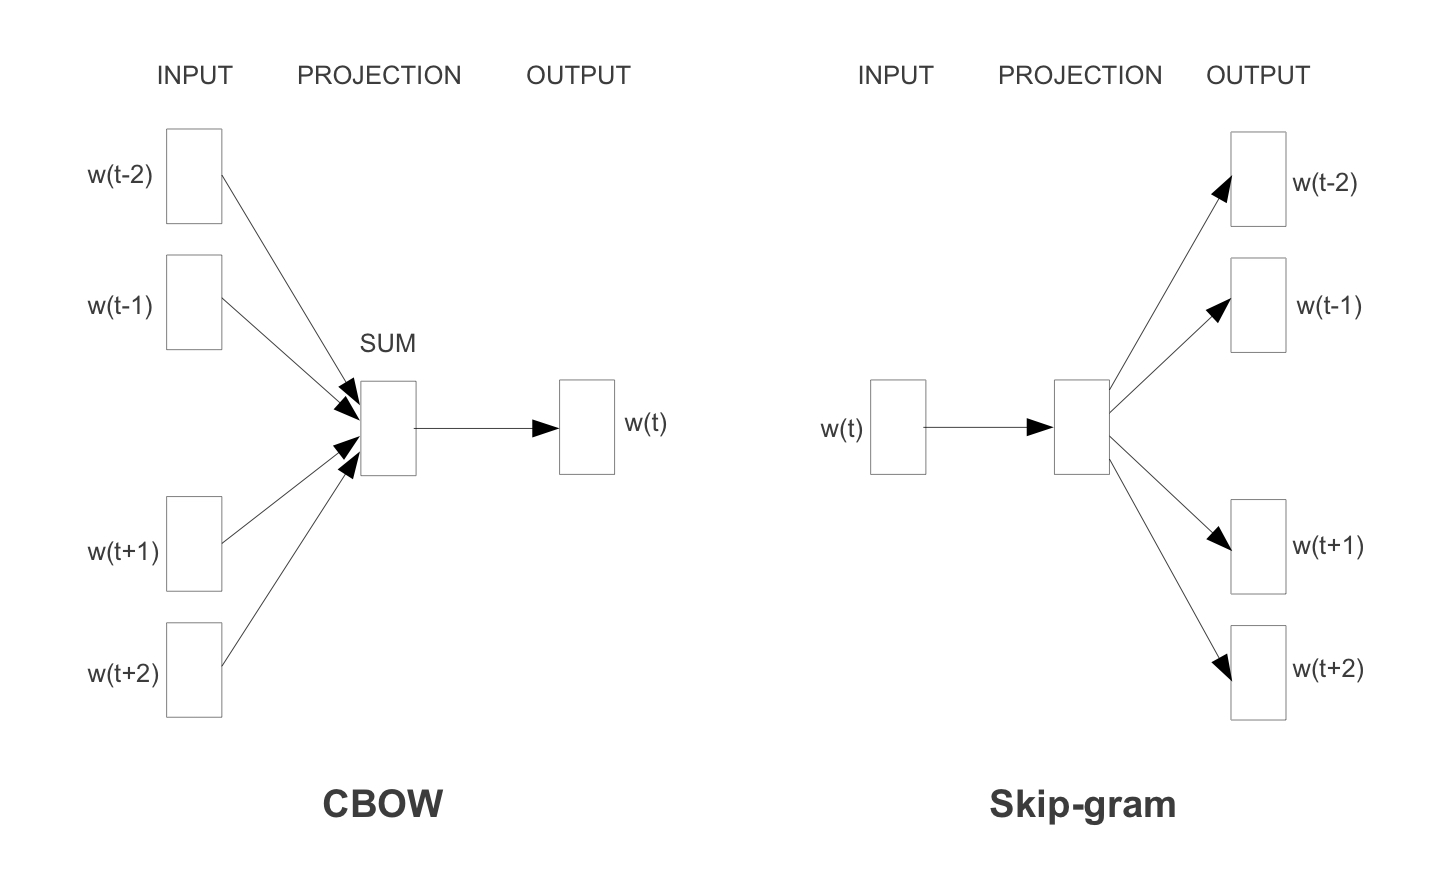
\includegraphics[width=12cm]{grafiken/cbow_skip_gram.jpeg}
\caption[Word2Vec Architekturen CBOW und SG]{Word2Vec Architekturen CBOW und SG aus \textcite[S. 5]{Word2Vec}}.
\label{CBOW_Skip_gram}
\end{center}
\end{figure}
\noindent Bereits in vorherigen Studien konnten \textcite{mikolov-etal-2013-linguistic} zeigen, dass semantisch ähnliche Wörter, aufgrund ihrer ähnlichen internen Repräsentation im Vektorraum nah beieinander liegen\footnote{Die Semantik ist ein Teilgebiet in der Linguistik und bezeichnet die Studie um die inhaltliche Bedeutung von Zeichenfolgen wie sie in Wörtern, Phrasen, Sätzen oder Dokumenten vorkommen \parencite{Jurafsky:2009:SLP:1214993}. Die Bedeutung von lexikalischen Einheiten, beispielsweise von Wörtern, wird lexikalische Semantik genannt. Semantisch ähnliche Wörter sind auf ihre Semantik bezogen ähnlich. Beispielsweise sind die Verben \textit{fiedeln} und \textit{geigen} bedeutungsähnlich (jedoch nicht bedeutungsgleich). \textit{Musizieren} ist ebenso bedeutungsähnlich und würde im Vektorraum idealerweise nah bei den das Geigenspiel beschreibenden Wortvektoren liegen, während beispielsweise \textit{marschieren} im Vektorraum weiter entfernt wäre.}.\\
Ein vielzietiertes Beispiel dafür ist die algebraische Operation  \textit{vector(„king“) - vector(„man“) + vector(„woman“) ≈ vector(„queen“)} \parencite[vgl.][1]{mikolov-etal-2013-linguistic}. Diese beruht auf der Analogie \textit{king - queen = man - woman} (gesprochen „king verhält sich zu queen wie man zu woman“).\\
Hervorzuheben ist, dass der bei der Addition bzw. Subtraktion von Wortvektoren entstandene Vektor nicht exakt einem Vektor aus dem Vokabular entsprechen muss. Im genannten Beispiel wird der Vektor für \textit{queen} aus dem Vokabular aufgrund der Nähe zum resultierenden Vektor ausgegeben.
\begin{figure}[H]
\begin{center}
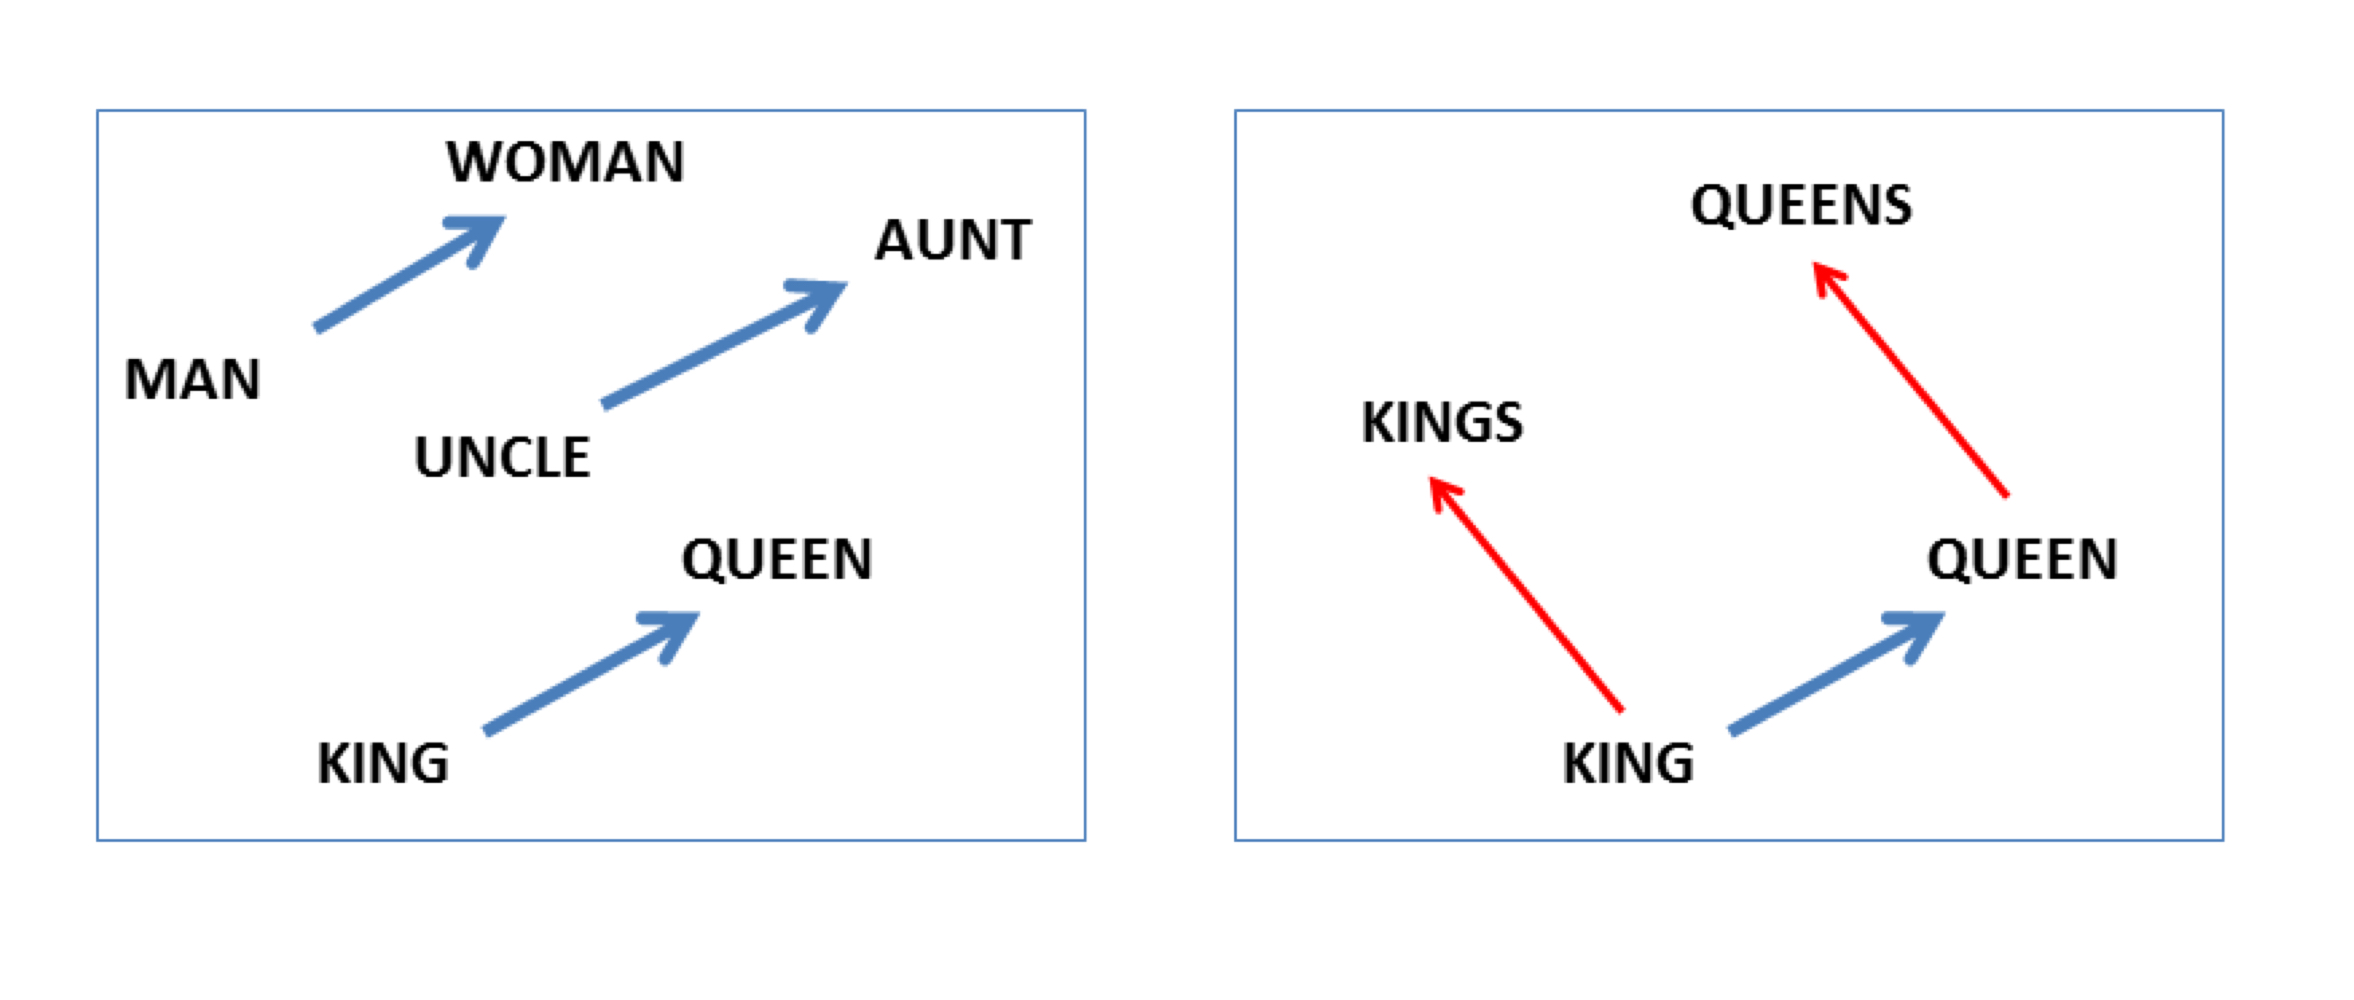
\includegraphics[width=12cm]{grafiken/king_queen_analogy.jpeg}
\caption[Wortvektoren Relationen im 2-dimensionalen Vektorraum]{Wortvektoren Relationen im 2-dimensionalen Vektorraum aus \textcite[5]{mikolov-etal-2013-linguistic}}.
\label{king_queen}
\end{center}
\end{figure}
\noindent Sowohl Word2Vec, als auch weitere zeitlich nah darauf folgende Modelle, wie GloVe \parencite{pennington2014glove}, lernen Word Embeddings auf Wortebene, was den Nachteil hat, dass nur Wörter, die in der Trainingsmenge existierten, vorhergesagt werden können. An dieser Stelle setzt die folgende Worteinbettungstechnik an.

\subsubsection{fastText} \label{fT_grundlage}
Im Jahr 2016 erschien der Artikel „Enriching Word Vectors with Subword Information“ von Forschungsgruppe des Facebook AI Research Labs unter \textcite{DBLP:journals/corr/BojanowskiGJM16}. Die Autoren stellten dort die Open-Source-Bibliothek fastText vor. FastText begreift sich als Erweiterung der Word2Vec Skip-gram-Architektur um das Training auf kleineren linguistischen Einheiten (\cite{DBLP:journals/corr/BojanowskiGJM16}). FastText zerlegt ein Wort in seine n-Gramme, also Zeichensequenzen der Länge n, und berechnet für diese Vektorrepräsentationen. Für das Wort \textit{Musik} und n=3 würde der Sack der zu \textit{tri}-Grammen zusammengefassten Zeichen wie folgt aussehen: <Mu, Mus, usi, sik, ik>. 
Eine Wortrepräsentation setzt sich aus der Summe der Vektoren der zu n-Grammen zusammengefassten Zeichen des Wortes zusammen.\\
Der Vorteil dieser Methode ist, dass selbst Wörter, die nicht in den Trainingsdaten vorkommen, also \textit{Out-Of-Vocabulary} (OOV) Wörter, betrachtet werden können. Besonders profitieren Sprachen wie Deutsch, mit sehr vielen morphologisch-komplexen\footnote{Die Morphologie beschäftigt sich als Teilgebiet der Linguistik mit Wortformen.} Wörtern, von dem Training auf n-Gramm-Ebene, da bestenfalls n-Gramme des unbekannten Wortes schon vom Modell gelernt wurden und daraus eine Vektorrepräsentation des ganzen Wortes gebildet werden kann. Aus den n-Grammen des Beispielworts \textit{Musik} könnten dabei Vektorrepräsentationen vieler weiterer OOV-Wörter abgeleitet werden (\textit{musisch}, \textit{Musikwissenschaft}, \textit{unmusikalisch} usw.).

\subsubsection{Sprachübergreifende fastText-Embeddings} \label{grundlage_muse}
Das Training von Word Embeddings (s. Kapitel \ref{Word Embeddings}) findet auf sprachspezifischen Korpora statt. Im Jahr 2013 erkannten \textcite{mikolov2013exploiting}, dass die Word2Vec-Embeddings verschiedener Sprachen in ihren jeweiligen Vektorräumen ähnliche Strukturen aufwiesen. \\
Sprachübergreifende Word Embeddings in einem gemeinsamen Vektorraum ermöglichen zum einen den sprachübergreifenden Vergleich von Wortbedeutungen und zum anderen den Transfer von gelerten semantischen Zusammenhängen von Sprachen mit einer reicheren Datengrundlage zu Sprachen mit weniger zur Verfügung stehenden Daten \parencite{ruder2019survey}.
\textit{Vector Space Alignment} von monolingualen Word Embeddings ist eine Methode sprachübergreifende Word Embeddings zu erhalten.\\
\\
 Ende 2017 hat Facebook AI Research (FAIR) eine mit \textit{„MUSE: Multilingual Unsupervised and Supervised Embeddings“} Methode für das lineare Mapping von monolingualen \textit{source} auf monolinguale \textit{target} fastText-Embeddings vorgestellt \parencite{conneau2017word}. Im Gegensatz zu vorher entwickelten Methoden gelingt dies auf eine unüberwachte Art, nämlich ohne einen parallelen Datensatz, oder bilinguale Lexika. Die Autoren stellen vortrainierte auf fastText basierenden Embeddings zum Download zur Verfügung \parencite{conneau2017word}. Außerdem lassen sich mit dem veröffentlichten Code selbst trainierte monolinguale fastText-Embeddings einander angleichen.
\begin{figure}[H]
\begin{center}
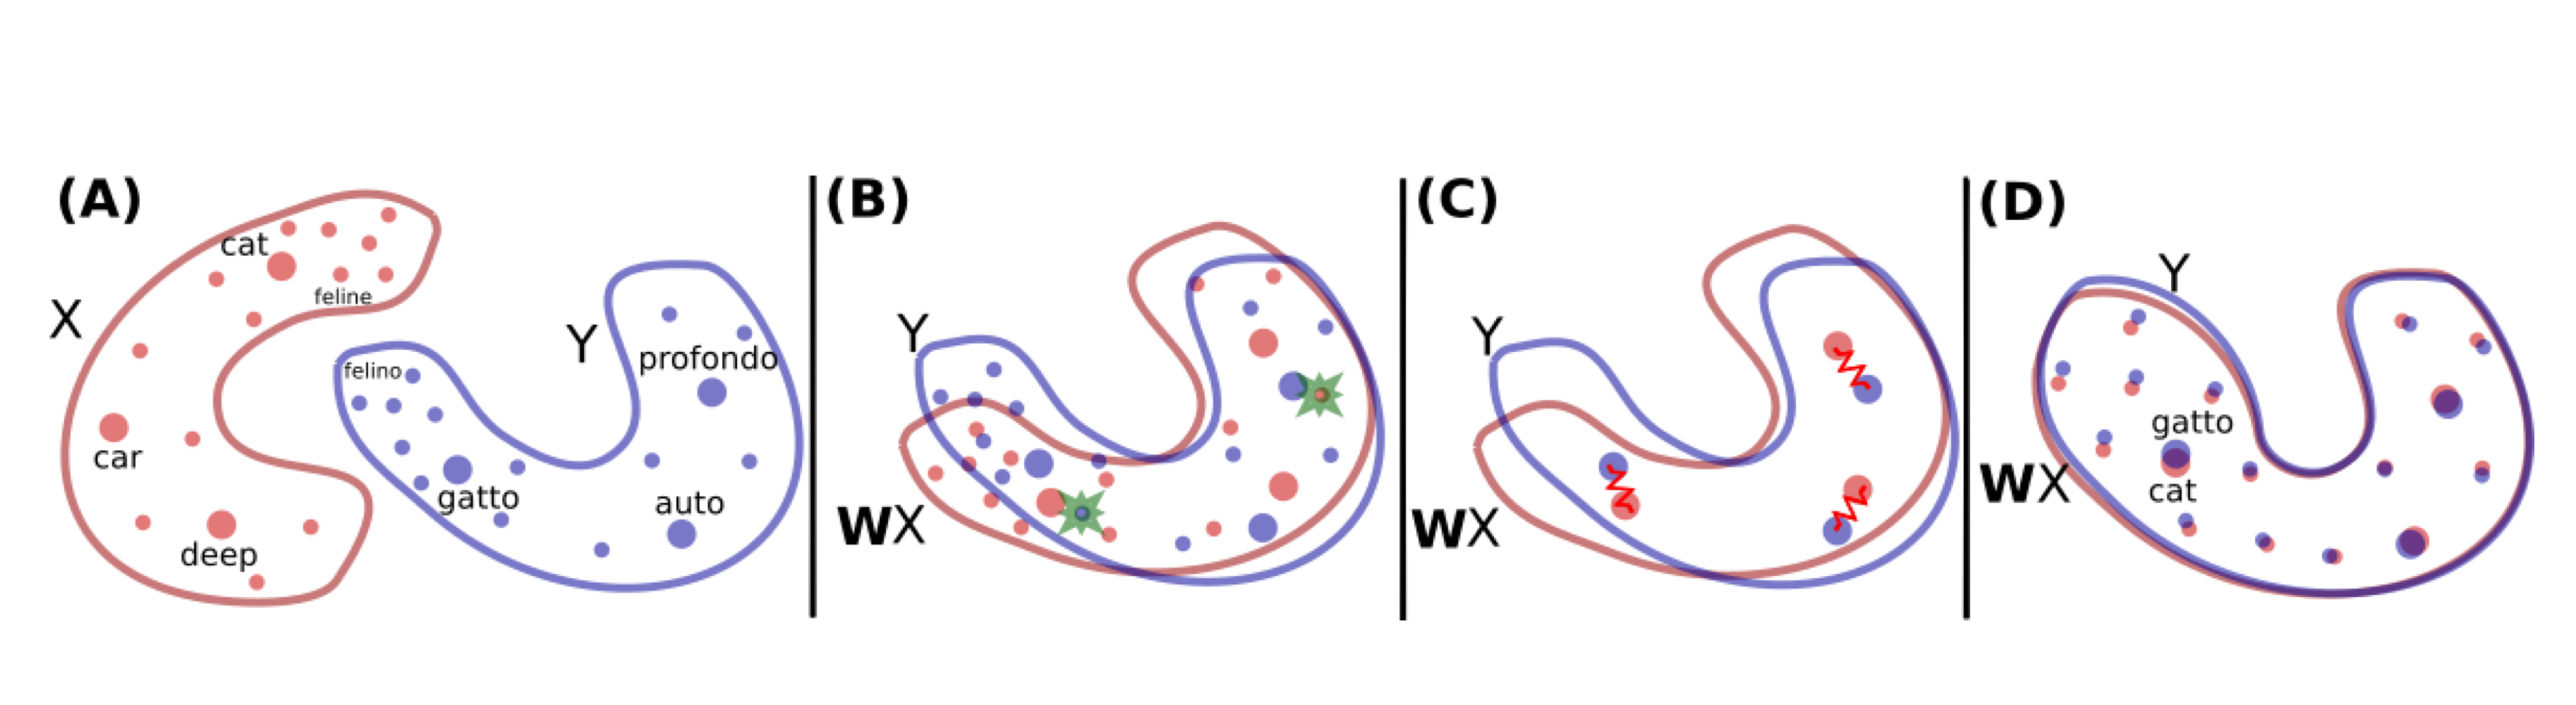
\includegraphics[width=16cm]{grafiken/MUSE_method.jpeg}
\caption[Illustration der Vektorraum Alignment Methode]{Illustration der Vektorraum Alignment Methode aus \textcite[3]{conneau2017word}}.
\label{MUSE}
\end{center}
\end{figure}
\noindent Im Folgenden wird eine Intuition für die vorgenommenen Schritte anhand der Illustration in Abbildung \ref{MUSE} gegeben.\\ 
\\
Bild \textbf{(A)} stellt die Ausgangssituation zweier Distributionen von monolingualen Word Embeddings $X$ und $Y$ im Vektorraum dar, wobei rote Punkte für englische und blaue Punkte für italienische Wörter stehen.\\
Seien \(X = x_1, \ldots, x_n\) und \(Y = y_1, \ldots, y_m\) die $n$ bzw. $m$ sprachspezifischen Word Embeddings.
Das Ziel ist das Lernen eines linearen Mappings \(WX = Wx_1, \ldots, Wx_n = Y\). Dabei sollen die „inneren Strukturen“ der Distributionen $X$ und $Y$ erhalten bleiben \parencite[3]{conneau2017word}.\\
\\
Zunächst wird eine Rotationsmatrix $W$ gelernt, die zum groben Alignment von $X$ und $Y$ führt \textbf{(B)}. Dafür wird \textit{Adversarial Learning} implementiert, welches ein Ansatz des unsupervised Machine Learning ist. Einem \textit{Discriminator} wird hierbei zufällig ein Datensatz aus \(WX\) oder $Y$ übergeben und seine Aufgabe ist es zu entscheiden, von welcher Quelle der Datensatz kommt. Die zufällig ausgewählten Datensätze werden in Abb. \ref{MUSE} durch grüne Sterne dargestellt. Es entsteht ein „Wetteifern“, denn während der \textit{Discriminator} seine Fähigkeit maximiert korrekt zu entscheiden, verbessert der sog. \textit{Generator} (hier $W$) seine künstlichen Datensätze, indem er \(WX\) möglichst an $Y$ annähert \parencite{conneau2017word}.\\
\\
Die so entstandene Matrix $W$ wird nun in einem iterativen Prozess verbessert \textbf{(C)}. Dafür wird aus Wörtern, die häufig auftreten (in Abb. \ref{MUSE} fett dargestellt) und ihren k-nächsten Nachbarn ein bilinguales Wörterbuch gebildet. Sie dienen somit als Ankerpunkte für das Mapping. Auf dem Wörterbuch wird der Procrustes Algorithmus iterativ angewendet \footnote{Die Autoren verweisen auf \textcite{artetxe-etal-2017-learning}.}, um die Qualität des Wörterbuchs zu erhöhen \parencite{conneau2017word}. Schließlich wird das verbesserte Mapping auf alle Wörter angewendet.\\
\\
Im letzten Schritt \textbf{(D)} findet die Übersetzung mittels $W$ unter der Benutzung des Ähnlichkeitsmaß $CSLS$ (Cross-domain Similarity Local Scaling) statt. Letzteres dient der Entzerrung von dichten Stellen um bestimmte Wörter, wie um das Wort „cat“ auf dem ersten Bild von Abbildung \ref{MUSE} \parencite{conneau2017word}.\\
Sei \(Wx_s\) das Mapping eines Word Embeddings der \textit{source} Sprache. Und sei \(N_t(Wx_s)\) seine Nachbarschaft mit k Nachbarn. Dann notieren \textcite[vgl.][4]{conneau2017word} die durschnittliche Ähnlichkeit einer \textit{source} Embedding \(x_s\) zu seiner \textit{target} Nachbarschaft als 
\[r_T(Wx_s) = \frac{1}{K} \sum_{y_t\in{N_t}(Wx_s)} \cos(Wx_s,y_t),\]
wobei die Kosinus-Ähnlichkeit zum Einsatz kommt, ein Maß für die Ähnlichkeit zweier Vektoren. Die durschnittliche Ähnlichkeit zu den Nachbarwörtern wird für alle \textit{source} und \textit{target} Embeddings ausgerechnet. Dann werden die erhaltenen Werte eingesetzt in die Berechnung für die Ähnlichkeit von \(Wx_s\) und einer \textit{target} Embedding \(y_t\):
\[CSLS(Wx_s,y_t) = 2\cos(Wx_s,y_t)\ - \ r_T(Wx_s)\ - \ r_S(y_t)\]
$CSLS$ verringert so die Ähnlichkeit von Wortvektoren in dichten Umgebungen \parencite{conneau2017word}. 
\newpage
\subsubsection{Problematik statischer Word Embeddings} \label{Word_Embeddings_problematik}
Alle bisher besprochenen Methoden berechnen für jedes Wort genau eine Vektorrepräsentation. Problematisch wird dies bei mehrdeutigen Wörtern. Beispielsweise kann das Wort \textit{Ton} sowohl ein plastisch verformbares Material zur Herstellung von Gegenständen, als auch eine durch das Gehör wahrnehmbare Luftschwingung beschreiben.\\
Die \textit{statischen} Word Embeddings von Word2Vec, GloVe und fastText könnten diesen Umstand nicht mit verschiedenen Vektoren für \textit{Ton} modellieren.

\subsection{Contextual Word Embeddings}
Im Jahr 2018 revolutionierten \textit{Embeddings from Language Models} (ELMo) \parencite{ELMo} die Word Embedding Modelle, indem jedes Wort eine eigene Vektorrepräsentation abhängig vom Kontext bekommt. Kontext bedeutet für ELMo nun auch die Position des Wortes im Dokument. ELMo nutzt dafür \textit{Rekurrente Neuronale Netze} (RNNs), deren Zustände die Eigenschaft haben, abhängig von vorhergehenden Zuständen zu sein und folglich auch nachfolgende Zustände zu beeinflussen. Je nach Stelle im Satz entsteht durch das unidirektionale Training mit RNNs eine andere Worteinbettung.\\
Eine Anwendung von RNNs außerhalb des Natural Language Processing liegt beispielsweise auch in der Generierung von Notentexten, welche durch die positiven Eigenschaften der RNNs für die Verarbeitung von Sequenzen erleichtert wird \parencite{DUA2020465}.

\subsubsection{BERT}
Im Jahr 2019 wurden \textit{Bidirectional Encoder Representations from Transformers} (BERT) von Devlin u.a. (2019) eingeführt. Auch BERT generiert \textit{Contextual Word Embeddings}. Allerdings nutzt BERT dafür keine RNNs, sondern dem neuen Stand der Technik entsprechenden \textit{Transformer}-Blöcke. Die Transformer-Architektur wurde schon ein Jahr vor ELMo von \textcite{https://doi.org/10.48550/arxiv.1706.03762} vorgestellt. BERT verwendet für das Training die Enkodierer-Blöcke der Transformer mit einem tiefen Netzwerk aus entweder 12 oder 24 Schichten. Das Konzept der Selbstattention der Transformer hilft BERT dabei, den Fokus bei der Berechnung der Wortvektoren auf wichtige Wörter zu setzen.\\
BERT setzt auf das Nutzen von auf großen, unannotierten Datensätzen und für spezielle Tasks vortrainierten Architekturen. Durch \textit{Finetuning}, also Feinabstimmungen bestimmter Hyperparameter, können diese für \textit{Downstream Tasks}, wie der Task der Textklassifikation, angepasst werden \parencite{devlin-etal-2019-bert}. Im Kapitel \ref{TC_BERT} des Hauptteils dieser Arbeit werden die für das Finetuning infrage kommenden Hyperparameter beschrieben.
\begin{figure}[H]
\begin{center}
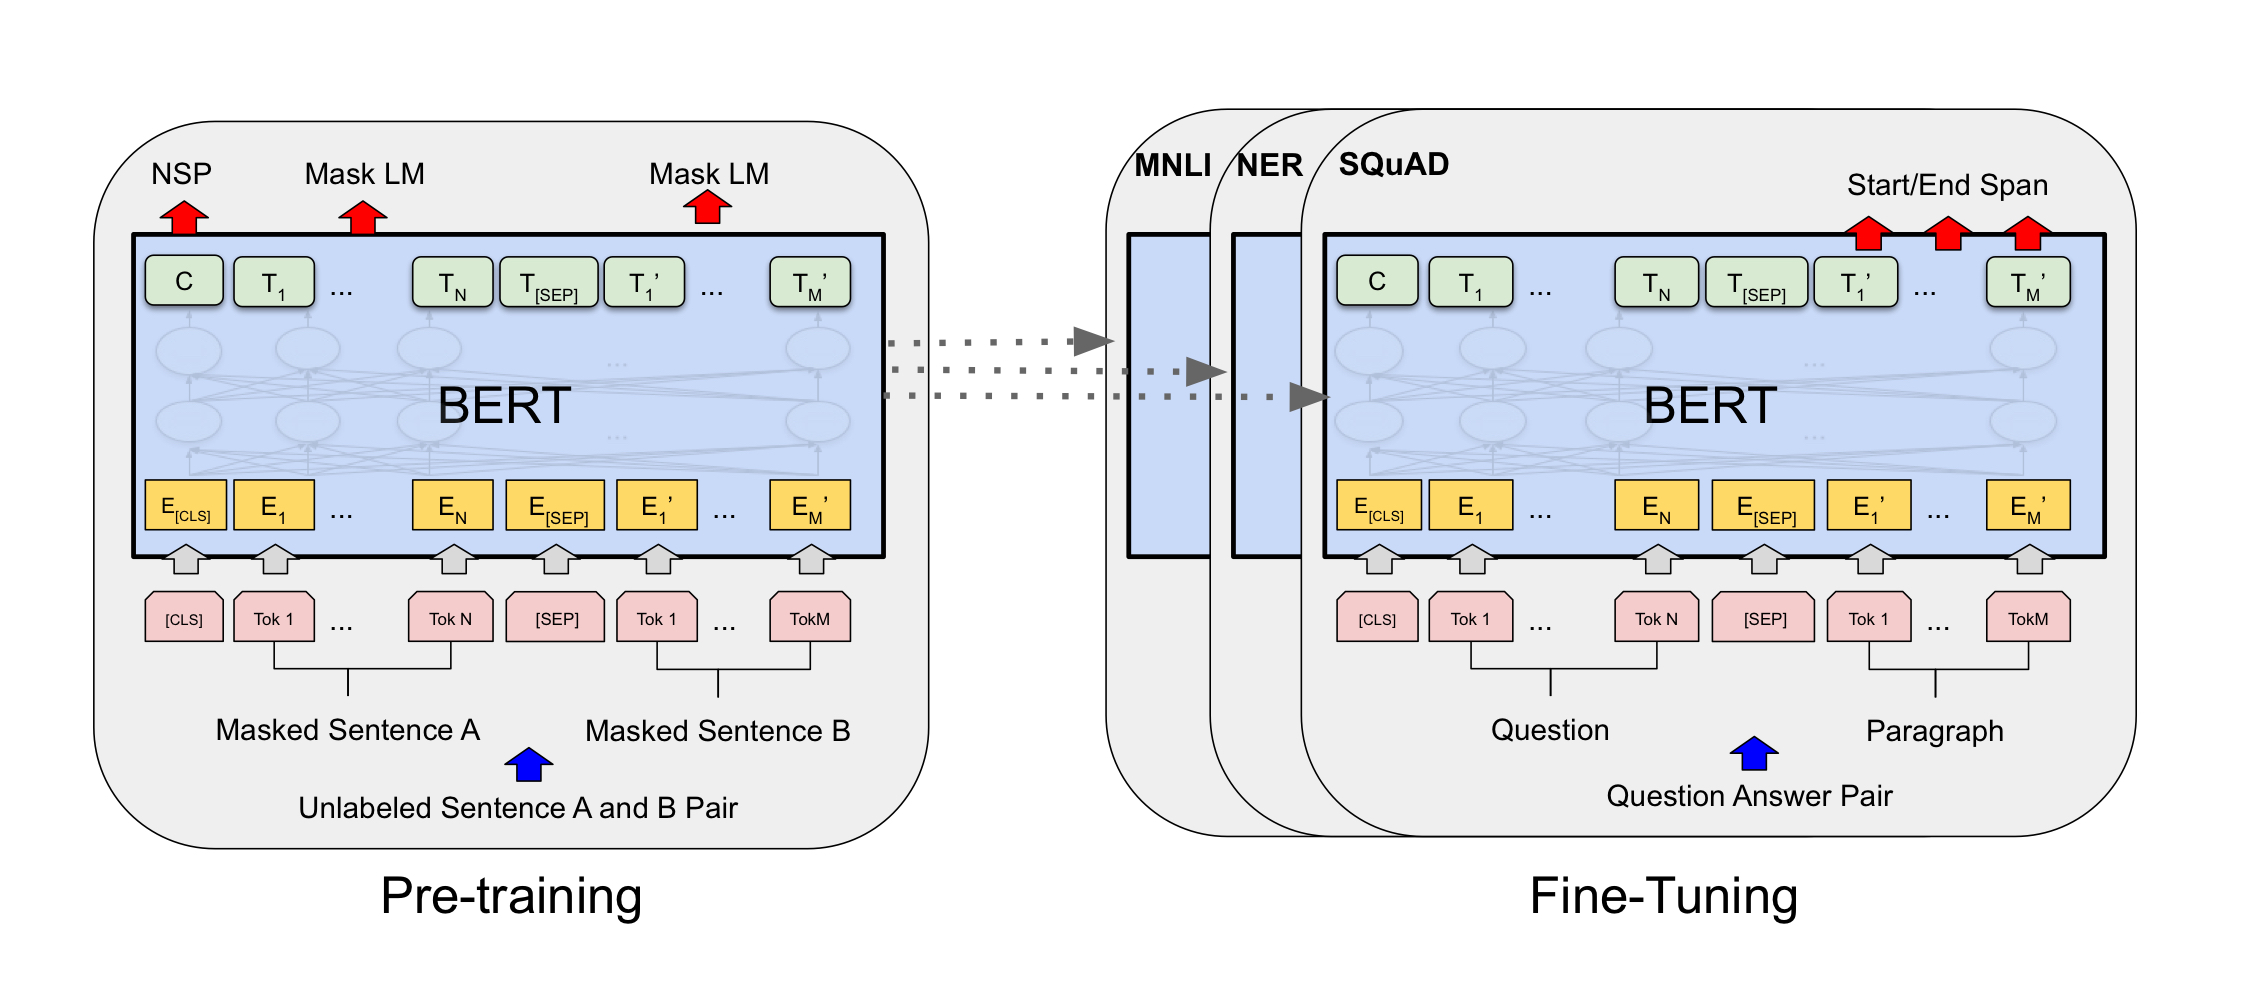
\includegraphics[width=16cm]{grafiken/BERT_Architektur.jpeg}
\caption[Pre-Training und Finetuning der BERT Modelle]{Pre-Training und Finetuning der BERT Modelle aus \textcite[3]{devlin-etal-2019-bert}}.
\label{BERT_Architektur} 
\end{center}
\end{figure}
\noindent BERT nutzt maskierte Sprachmodellierung (MLM), eine Technik, die zufällig 15\% der Wörter in einer Eingabesequenz maskiert, um sie schließlich aus dem Kontext vorherzusagen \parencite{devlin-etal-2019-bert}. Dabei kann es sich bei der Eingabesequenz um einen einzelnen Satz, aber auch um einen Text bestehend aus mehreren Sätzen handeln \parencite{devlin-etal-2019-bert}. Im Gegensatz zu den RNNs wird die gesamte maskierte Sequenz auf einmal im Modell verarbeitet. Die zweite Technik, die BERT für das Training benutzt, ist die Vorhersage des Nächsten Satzes (NSP). Dafür erhält BERT zwei Sätze und sagt voraus, ob der zweite Satz zum Kontext des ersten gehört, wobei er in der Hälfte der Fälle ein zufällig gewählter Satz ist \parencite{devlin-etal-2019-bert}.\\
Das durch diese Techniken entstehende bidirektionale Training führt zu einem tieferen Lernen des Kontexts eines Wortes, da auch weitreichende Zusammenhänge in der Eingabesequenz erfasst werden können.
\subsubsection{Multilinguales BERT} \label{SBERT}
Eine der vielen Erweiterungen von BERT ist das multilinguale mBERT, das auf dem konkatenierten Wikipedia-Korpus 104 Sprachen trainiert wurde \parencite{bert_multi}. Das Modell wird in Kapitel \ref{BERT_Modelle} des Methodik-Teils beschrieben.

\subsubsection{SBERT}
Sentence-BERT (SBERT) \parencite{reimers-2019-sentence-bert} wurde im Jahr 2019 als Modifikation von BERT veröffentlicht. SBERT nutzt ein siamesisches Netzwerk, um Satzeinbettungen unter Beachtung der semantischen Kosinus-Ähnlichkeit generieren.\\
SBERT-Modelle werden auch Sentence Transformer genannt, da sie, mit BERT als Grundlage, ebenso auf Transformer-Blöcken basieren. Der Output von BERT für einen Satz geht bei SBERT über in ein \textit{Pooling Layer}, welches eine Satzrepräsentation von fester Größe, z.B. 768 Dimensionen für BERT-Base \parencite{devlin-etal-2019-bert}, generiert. Als \textit{mean-pooling} konfiguriert werden alle \textit{Contextual Word Embeddings} für die Wörter des Satzes des BERT Outputs gemittelt.
\begin{figure}[H]
\begin{center}
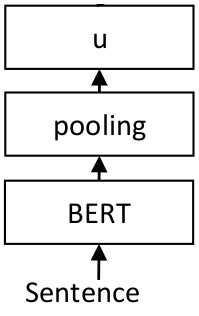
\includegraphics[width=3cm]{grafiken/SBERT_Architecture.png}
\caption[Architektur eines Sentence Transformers]{Architektur eines Sentence Transformers,\\
https://www.sbert.net/docs/training/overview.html, letzter Zugriff:\\ 21.11.2022 (Screenshot vom 21.11.2022, 20:34 Uhr)}.
\label{SBERT_Architektur}
\end{center}
\end{figure}
\noindent Die Autoren zeigen, dass SBERT für Tasks, die die semantische Ähnlichkeit fokussieren, besser als BERT und die aus dem Durchschnitt von fastText-Wortvektoren gebildete Satzvektoren abschneidet \parencite{reimers-2019-sentence-bert}. Genau wie BERT-Modelle werden auch SBERT-Modelle vortrainiert und \textit{out-of-the-box} anwendbar zur Verfügung gestellt.

\section{Themenmodellierung mit BERTopic} \label{Grundlage_Topic_Modeling}
Themenmodellierung (\textit{Topic Modeling}) beschreibt die Machine Learning Task des Findens von Themenwörtern zur Beschreibung der Inhalte von Dokumenten eines Textkorpus. Sie zählt zum unüberwachten Lernen (\textit{unsupervised learning}) und ihre Ergebnisse benötigen menschliche Expertise, um gedeutet zu werden.\\
Da der Fokus der Bachelorarbeit nicht auf dem Topic Modeling liegt, wird die verwendete Topic Modeling Methode BERTopic nur grob vorgestellt. Für ein tiefergehendes Verständnis lohnt sich ein Blick in die hier zitierte Literatur.\\
BERTopic \parencite{bertopic} nutzt state-of-the-art vortrainierte Embedding-Modelle, um Themen zu generieren. \\
die Themen aus Dokumenten extrahiert, indem sie Wörter mit ähnlichen Bedeutungen zu Clustern zusammenfasst. \\
BERTopic nutzt in seiner Standardkonfiguration folgende Pipeline \parencite{bertopic}:
\begin{itemize}
\item \textit{Embeddings}
\item \textit{Dimensionality Reduction}
\item \textit{Clustering}
\item \textit{Topic Representation}
\end{itemize} 
Für die Extraktion der Embeddings werden state-of-the-art vortrainierte Sentence-BERT Modelle (s. Kapitel \ref{SBERT}) genutzt.\\
Bevor das Clustering durchgeführt werden kann, muss die Dimensionalität der Embeddings reduziert werden, da die großen Dimensionen der generierten Embeddings den Clustering Algorithmen Probleme bereiten können \parencite{bertopic}. In der Standardkonfiguration von BERTopic geschieht dies mit dem UMAP-Algorithmus, welcher die Kosinus-Ähnlichkeit als Distanzmetrik benutzt \parencite{UMAP}.\\ 
Der genutzte Clustering-Algorithmus ist HDBSCAN \parencite{HDBSCAN}.
Alle Dokumente eines Clusters werden dann zu einem Dokument zusammengefasst, welches das Cluster repräsentiert. Durch Zählen der Häufigkeiten des Vorkommens von Wörtern im Cluster wird eine BoW-Repräsentation gebildet. Im Kapitel \ref{BOW} wurde die Idee von BoW beschrieben, allerdings wird die Technik hier auf die Cluster und nicht auf die einzelnen Dokumente angewendet, damit die Wörter auf Topic-Ebene herausgestellt werden können \parencite{bertopic}.\\
Die eigentliche Repräsentation der Topics wird schließlich mit c-TF-IDF, einer clusterbasierten Version von TF-IDF (s. Kapitel \ref{TF-IDF}). TF-IDF kann auf einer Liste von Dokumenten angewendet, die Relevanz der Wörter zwischen den Dokumenten vergleichen. c-TF-IDF bekommt die BoW-Repräsentation eines Clusters als Eingabe und kann somit die Relevanz der Wörter in den verschiedenen Clustern bewerten und schließlich die relevantesten Wörter eines Clusters als Topic zusammenfassen \parencite{bertopic}. 
\begin{figure}[H]
\begin{center}
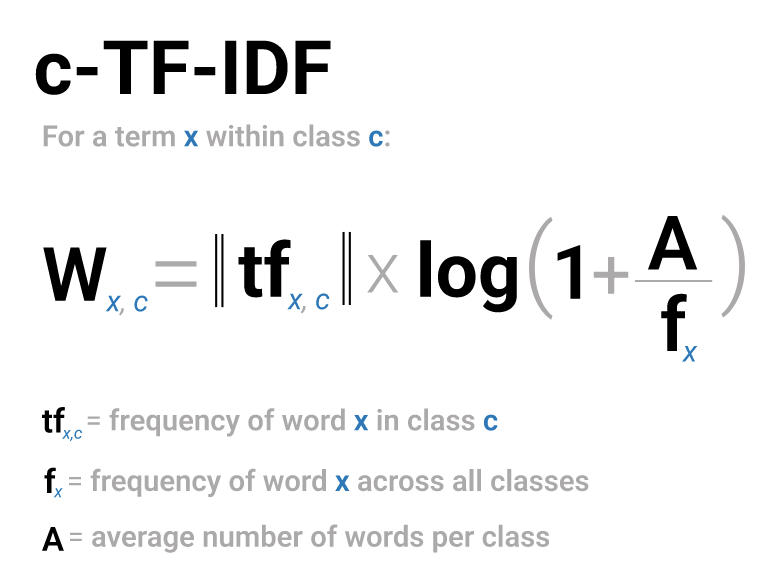
\includegraphics[width=8cm]{grafiken/c-tf-idf.png}
\caption[BERTopic nutzt c-TF-IDF für die Topic Repräsentation]{BERTopic nutzt c-TF-IDF für die Topic Repräsentation, \\https://maartengr.github.io/BERTopic/algorithm/algorithm.html\#3-cluster-documents, letzter Zugriff: 16.11.2022 (Screenshot vom 16.11.2022, 14:01 Uhr)}.
\label{Pipeline}
\end{center}
\end{figure}
\noindent BERTopic ermöglicht es, die beschriebene Pipeline \textit{out-of-the-box} anzuwenden. Es ist je nach Nutzen für den Anwendungsfall allerdings auch möglich, die Standardkonfiguration zu verändern, etwa indem andere Word Embedding Modelle, oder PCA für die Reduzierung der Dimensionen genutzt werden.\\
\\
Das Ergebnis des Topic Modelings mit BERTopic sind dichte Cluster von Wörtern, aus denen Topics interpretiert werden können. Die Ausgabe als „Worte-Cluster“ hat gegenüber einem einzigen Wort den Vorteil, dass der Kontext des Wortes erkennbar wird. Bezug nehmend auf das Beispiel im Abschnitt \ref{Word_Embeddings_problematik}, könnte somit korrekt interpretiert werden, um welche Bedeutung es sich bei \textit{Ton} handelt, wenn sich das Wort in demselben Cluster wie \textit{Klang}, \textit{Tonkunst} und \textit{Musik} befindet.
\section{Textklassifikation mit Machine Learning Methoden} \label{tc_pipeline}
Textklassifikation beschreibt die Task der Zuordnung von Dokumenten zu vordefinierten Kategorien und kann folgendermaßen formal notiert werden:\\
Für eine Menge von Dokumenten \textit{D} und einer Menge von Kategorien \textit{{c\textsubscript{1}, c\textsubscript{2}, ..., c\textsubscript{n}}} wird jedem Dokument \textit{d\textsubscript{i}} genau eine Kategorie \textit{c\textsubscript{j}} zugewiesen \parencite[vgl. S. 1]{ikonomakis}.\\
\textcite{ikonomakis} unterscheiden dabei \textit{text genre classification} von \textit{text topic-based classification}. Ein prominenter Korpus für die \textit{text genre classification} ist der 20 Newsgroups Korpus, welcher Dokumente aus 20 Nachrichten-Kategorien, wie Sport und Weltnachrichten, umfasst. Diese Bachelorarbeit beschäftigt sich mit der \textit{text topic-based classification}. Die Texte dieser Textklassifikationsform haben die Eigenschaft aus ähnlichen Quellen zu stammen und in Format, Vokabular und Schreibstil weitgehend übereinzustimmen \parencite{ikonomakis}.\\
Die automatische (maschinelle) Textklassifikation ist eine Machine Learning Task des überwachten Lernens (\textit{supervised learning}).\\
Anhand schon klassifizierter Daten berechnet ein lernender Algorithmus Strukturen. Diese ermöglichen es dem Klassifikationsalgorithmus auf unbekannten Daten, die Klasse mit möglichst hoher Gewissheit zu entscheiden. Die Gewissheit der Klassifikation wird bei der \textit{weichen Klassifikation} mit einer bestimmten Prozentzahl angegeben. In dieser Bachelorarbeit wird allerdings eine binäre Entscheidung für eine Klasse erzwungen, was auch \textit{harte Klassifikation} genannt wird.\\
Für das Training des lernenden Algorithmus wird üblicherweise eine Teilmenge der insgesamt zur Verfügung stehenden Daten mit bekanntem Label genutzt, während die Güte des Klassifizierers auf den restlichen Daten überprüft wird. Man spricht daher von \textit{Trainings-} und \textit{Testdaten}. Die Einteilung des Datensatzes wird  \textit{train-test-split} genannt, wobei auf einem Großteil der Daten trainiert und auf der kleineren Teilmenge getestet wird.
\begin{figure}[H]
\begin{center}
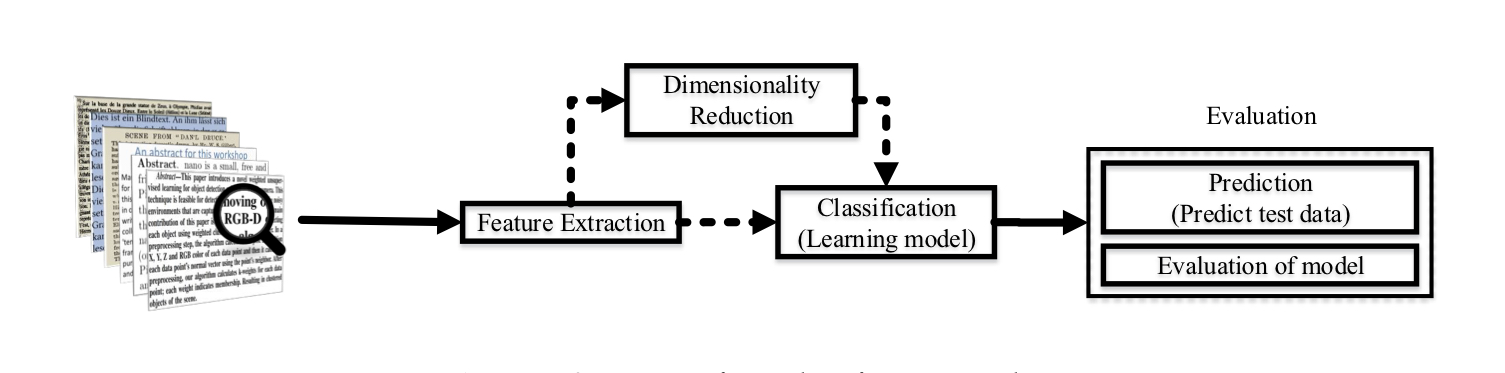
\includegraphics[width=14cm]{grafiken/text_classification_pipeline_kowsari.jpeg}
\caption[Text Classification Pipeline]{Text Classification Pipeline aus \textcite[S. 2]{Kowsari_2019}}.
\label{Pipeline}
\end{center}
\end{figure}
\noindent \textcite{Kowsari_2019} teilen die Pipeline der Textklassifikation grob in die folgenden vier Schritte ein (siehe Abbildung 2.2.):
\begin{itemize}
\item \textit{Feature Extraction}
\item \textit{Dimensionality Reduction}
\item \textit{Classifier Selection}
\item \textit{Evaluations}
\end{itemize} 
Der zweite Schritt ist laut \textcite{Kowsari_2019} optional und bezieht sich auf Techniken zur Reduzierung der Dimensionen, wie \textit{Principal Component Analysis} (PCA) oder \textit{Linear Discriminant Analysis} (LDA). Um den Rahmen dieser Bachelorarbeit nicht zu sprengen, wurde der Schritt nicht durchgeführt.\\
Das Textklassifikationssystem kann auf verschiedenen Textebenen angewendet werden, nach als Klassifikation von Dokumenten, Paragraphen, Sätzen oder Phrasen \parencite{Kowsari_2019}. In dieser Bachelorarbeit wird die Textklassifikation auf Dokumentenebene\footnote{Da es sich bei den Texten um Wikipedia-Artikel handelt, wird im Hauptteil dieser Bachelorarbeit anstatt von „Dokumentenebene“ von „Artikelebene“ gesprochen. „Dokumente“ steht hingegen für eine Liste von Texten, welche sowohl Artikel, Paragraphen, als auch Sätze sein können. Diese Terminologie nutzt auch das Topic Modeling (s. Kapitel \ref{Grundlage_Topic_Modeling})} durchgeführt.

\subsection{Feature Extraction}
Dieser Schritt dient der Umwandlung der natürlichsprachlichen Texte in eine Form, die einen geeigneten Input, für den Machine Learning Algorithmus darstellt, die sog. genannten \textit{Features}. Dabei ist die Wahl der richtigen Features essenziell und bei zu vielen Features kann das Problem des Overfittings entstehen \parencite{Kowsari_2019}.\\
Features können beispielsweise  Word Embeddings sein, welche mit Feature-Extraction-Techniken wie Word2Vec \parencite{Word2Vec} erzeugt werden. Dies werden detailliert im Kapitel \ref{Textrepräsentation} des Grundlagenkapitels behandelt.\\
Doch bevor die Features erzeugt werden, ist es für viele dieser Techniken unerlässlich, die Daten zu bereinigen \parencite{Kowsari_2019}. In dieser Arbeit wurden dafür Stoppwörter und Punktierungszeichen entfernt. Außerdem wurden die NLP-Techniken Stemming und Tokenisierung angewendet. Im Kapitel \ref{Datenbereinigung} kann dieser Prozess mit Beispielen aus dem Datensatz nachvollzogen werden, weshalb die einzelnen Schritte hier nicht erklärt werden.

\subsection{Wahl des Klassifikationsalgorithmus}
Die Wahl des besten Klassifikationsalgorithmus (auch Klassifikator genannt), ist \textcite{Kowsari_2019} zufolge der wichtigste Schritt der Klassifikationspipeline.
Für diese Arbeit wurden zwei Klassifikationsalgorithmen ausgewählt, die für die Task der maschinellen Textklassifikation vielversprechende Ergebnisse erwarten lassen.

\subsubsection{Support Vector Machines}
\textit{Support Vector Machine} (SVM) ist ein linearer Klassifikator, der für die Task der Textklassifikation bevorzugt gewählt wird \parencite{manning2008introduction}. Das Ziel einer SVM ist es, in einem Vektorraum eine optimale Entscheidungsschranke zu ermitteln, um zwei Klassen voneinander zu trennen, und kann daher als binärer Klassifikator beschrieben werden. Optimal ist die Entscheidungsschranke, wenn die trennende Hyperebene von jedem Datenpunkt der Trainingsdaten maximal entfernt ist.\\
Die Erweiterung des Verfahrens für den Fall, dass die Trainingsdaten nicht linear trennbar sind, sieht vor, dass dennoch versucht wird, eine Hyperebene zwischen den Datenpunkten aufzuspannen und ein kleinstmöglicher Fehler toleriert wird. Alternativ könnten die Vektoren auf eine höhere Dimension gebracht werden, sodass sie linear trennbar sind \parencite{manning2008introduction}.
\begin{figure}[H]
\begin{center}
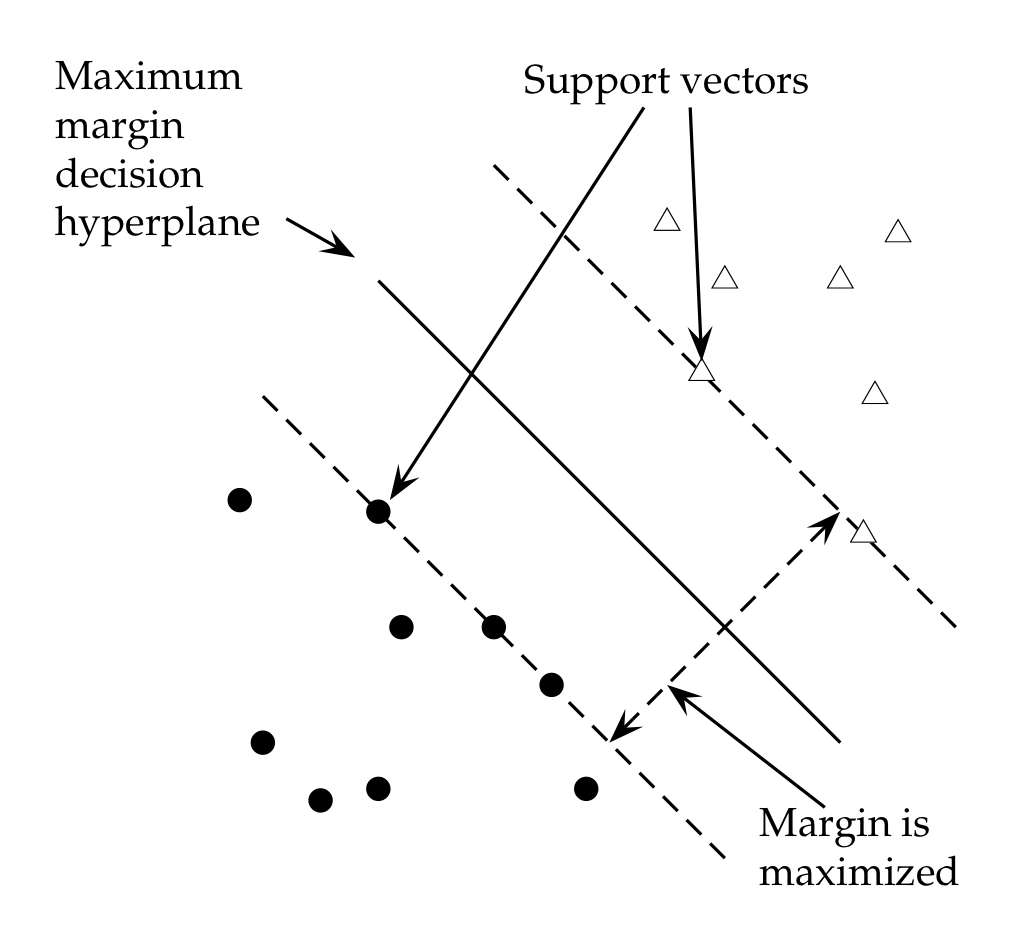
\includegraphics[width=8cm]{grafiken/SVM_Intro_IR_S.320.jpeg}
\caption[Support Vector Machine]{Support Vector Machine aus \textcite[S. 320]{manning2008introduction}}.
\label{SVM}
\end{center} 
\end{figure}
\noindent Abbildung \ref{SVM} illustriert das SVM-Verfahren für den linear separierbaren Fall. Die im n-dimensionalen Vektorraum geplotteten Datenpunkte zweier Klassen (Dreieck und Punkt) werden durch die zwischen den Stützvektoren (sog. \textit{Support Vectors}) aufgespannte Entscheidungsebene getrennt. Je weiter der Radius (\textit{margin}) um die Hyperebene, desto sicherer ist die Klassifikation eines Datenpunkts.

\subsubsection{Naïve Bayes} \label{NB}
\textit{Naïve Bayes} (NB) ist ein statistischer Klassifikator, welcher auf dem Satz von Bayes fundiert. Naïve Bayes bezeichnet eine Familie von Algorithmen. Hier ist genauer der \textit{Multinomial Naïve Bayes} gemeint.\\
Der Satz von Bayes berechnet für ein zu klassifizierendes Dokument \(\mathbf{d}\) und die Wahrscheinlichkeit in Klasse \(c\) zu sein wie folgt: \[P(c \mid \mathbf{d}) = \frac{P(c) \cdot P(\mathbf{d} \mid c)}{P(\mathbf{d})}, \] wobei \(\mathbf{d}\) durch einen Vektor \((x_1, \ldots, x_n)\) bestehend aus \(n\) \textit{features} repräsentiert wird und \(c\) eine mögliche Klasse der vordefinierten Klassen \(C\) ist.
\[P(c \mid \mathbf{d}) = P(c \mid x_1, \ldots, x_n)\]
Ein \textit{feature} \(x_i\), mit  \(1 \leq \ i \geq n\) könnte etwa die Wahrscheinlichkeit des Vorkommens eines bestimmten Wortes im Dokument sein \parencite{manning2008introduction}.\\
\textit{Naïve} wird der Klassifikator durch die Annahme genannt, dass die \textit{features} unabhängig voneinander eintreten. Aus der naiven Annahme folgt: \\
\[P(c \mid x_1, \ldots, x_n) = P(c \mid \mathbf{d}) = \frac{P(c) \cdot \prod_{i = 1}^{n}{P(x_i \mid c)}}{P(x_1) \cdot P(x_2)\cdot \ldots \cdot P(x_n)}\]
Das Ziel in der Textklassifikation ist, die beste Klasse für ein Dokument zu finden \parencite{manning2008introduction}.
\[c_{best} = \operatorname*{argmax}_{c \in C} P(c \mid \mathbf{d})\]
\subsection{Evaluationsmetriken} \label{Evaluationsmetriken}
Die Evaluation ist der letzte Schritt der Textklassifikationspipeline und dient dem Aufbauen eines Verständnisses dafür, wie gut die Vorhersagen des Modells sind (\cite{Kowsari_2019}).\\ 
Im Folgenden werden die in dieser Arbeit genutzten Evaluationsmetriken zur Bewertung der Güte der binären Klassifikation vorgestellt.\\
\\
\textbf{\textit{Accuracy}} gibt den Anteil der korrekten Vorhersagen unter allen Vorhersagen des Modells an.\\
\[Accuracy = \dfrac{Anzahl\ der\ korrekten\ Vorhersagen}{Anzahl\ aller\ Vorhersagen}\]
\\
Das Maß beschreibt allerdings nur bei etwa gleich großen Klassen zuverlässig die Güte des Modells. Bei stark unausgeglichenen Datensätzen könnte das Modell lernen, immer die übermäßig vorhandene Klasse vorherzusagen. Auch wenn es nicht ein einziges Mal die andere Klasse richtig vorhersagt, ist die Accuracy hoch.\\
\\
Deshalb wird zusätzlich der \textbf{\textit{F$_{1}$-Score}} verwendet. Er bemisst sich aus \textit{Precision} und \textit{Recall}.\\
\[Precision = \dfrac{Anzahl\ korrekter\ positiver\ Vorhersagen}{Anzahl\ aller\ positiven\ Vorhersagen}\]
\\
\[Recall = \dfrac{Anzahl\ korrekter\ positiver\ Vorhersagen}{Anzahl\ aller\ Vorkommen\ der\ positiven\ Klasse\ im\ Datensatz}\]
\\Das harmonische Mittel von Precision und Recall ergibt den F$_{1}$-Score.
\[F_{1} = 2 \cdot \dfrac{Precision \cdot Recall}{Precision + Recall}\]


\chapter{Forschungsstand}
Es konnte keine Arbeit gefunden werden, die ein in allen Aspekten vergleichbares Thema wie diese Arbeit behandelt. Mit einzelnen Aspekte dieser Arbeit in Verbindung stehende Forschungsliteratur wird im Folgenden dargestellt.

\section{Nutzung von Wikipedia für die Generierung von Trainingsdaten} \label{dl_in_dh}
\textcite{dl_in_dh} beschreiben zwei Herausforderungen, auf die Wissenschaftler im Bereich der digitalen Geisteswissenschaften\footnote{engl. \textit{Digital Humanities}; Der Begriff beschreibt das interdisziplinäre Aufeinandertreffen des weiten Feldes der Geisteswissenschaften (somit auch der Musikwissenschaft, und insbesondere der Linguistik) mit der Informatik. Für eine ausführliche Definition siehe \textcite{dig_hum}.} (DH) treffen, wenn sie \textit{supervised Machine Learning} und speziell das \textit{supervised Deep Learning} in ihrer Forschung nutzen wollen. Zum einen sei dies die Nicht-Verfügbarkeit von angemessenen Trainingsdaten. Entweder seien die Textressourcen zu spezifisch, und daher nicht ausreichend verfügbar, oder aber die Klassen der Trainingsdaten seien nicht ausgewogen verteilt. Zum anderen sei das \textit{Pre-Processing} der Daten im Bereich der digitalen Geisteswissenschaften notwendig, da die Textressourcen üblicherweise \textit{noisy}, aber auch uneinheitlich in ihrem Format seien.
Da große, frei verfügbare und bereits annotierte Datensätze bislang nicht von der DH-Community existierten, sei die beste Alternative, um Datensätze zu erstellen, immer noch der Mensch \parencite{dl_in_dh}.\\
\\
Wikipedia als Wissensbasis für semantische Informationen zu nutzen, ist keine neue Idee \parencite[s. bspw.][]{strube2006wikirelate}. Inwiefern der Wikipedia Korpus für die multilinguale Analyse genutzt werden kann, untersuchen \textcite{wiki_multilingual}. Die Autoren erhoffen sich vom Alignment ähnlicher Sätze in zwei Sprachen Einsicht darüber zu erlangen, wie bestimmte Themen in der Wikipedia in den verschiedenen Sprachen dokumentiert sind. Es sei möglich, vergleichbare Datensätze in verschiedenen Sprachen über die Linkstruktur der Wikipedia zu generieren, da Wikipedia-Artikel dasselbe Konzept beschreiben, auch wenn sie meist keine genauen Übersetzungen voneinander sind. Ihre Forschung betont, dass die Wikipedia durch ihre Linkstruktur ein großes Potenzial für die Generierung paralleler Korpora birgt \parencite{wiki_multilingual}.\\
\\
Aufwändig vortrainierte und frei zur Verfügung stehende Word Embedding Modelle, zum Beispiel von \textcite{pennington2014glove} und \textcite{mikolov2018advances}, sowie state-of-the-art Sprachmodelle \parencite{devlin-etal-2019-bert} verwendeten (neben weiteren Korpora) den Wikipedia-Korpus für das \textit{Pre-Training}.
\section{Vergleichsstudien zur multilingualen Textklassifikation}
\textcite{multilingual_tc_epidemic} vergleichen für die multilinguale Textklassfikation von Nachrichten zu Krankheitsausbrüchen verschiedene Machine Learning Modelle auf TF-IDF Wort-Gewichten mit multilingualen Deep Learning Modellen. Die Autoren beobachten, dass die Textklassifikation mit Machine Learning Klassifikatoren sehr unausgeglichene Ergebnisse produziert, mit den höchsten \textit{Precision}-Werten und den niedrigsten \textit{Recall}-Werten. Das Deep-Learning Sprachmodell BERT resultiert in stabileren Werten.\\
\\
\textcite{jiang2019cross} nutzen in einem sprachübergreifenden Vektorraum alignierte Word Embeddings in den Sprachen Englisch und Französisch und führen auf diesen Embeddings die Textklassifikation mit zwei verschiedenen Klassifikatoren, welche auf neuronalen Netzen basieren, aus. Sie beobachten, dass sowohl die monolingualen, als auch die bilingualen Klassifikationen vom sprachübergreifenden Vektorraum profitieren \parencite{jiang2019cross}.\\
\\
Eine kürzlich erschienene Studie von \textcite{mono_vs_multi_BERT} untersucht auf den Tasks der Textklassifikation, der Erkennung von Hassrede und der Sentimentanalyse, ob monolinguale (in Marathi) oder multilinguale vortrainierte auf BERT basierende Modelle besser abschneiden. Unter den untersuchten multilingualen Modellen befindet sich auch das in dieser Arbeit verwendete mBERT \parencite{devlin-etal-2019-bert}. Die Autoren beobachten, dass die monolingualen BERT-Modelle auf allen Datensätzen besser als die monolingualen BERT-Modelle abschneiden.

\section{Kombination von transformer-basiertem Topic Modeling und Word Embeddings für die Textklassifikation}
\textcite{alhaj2022improving} nutzen den Output von BERTopic, um Textrepräsentationen von Tweets anzureichern. Zunächst bilden sie eine Textrepräsentation Embedding($doc_d$) mit dem Durchschnitt der einzelnen Word2Vec-Embeddings aller Wörter im Dokument. Dann generieren sie die Verteilung von latenten Topics BERTopic($doc_d$) im Dokument $d$. Die Topic Repräsentation und die Word Embeddings eines Dokumentes werden nun konkateniert. Die so erhaltene Dokumentrepräsentation (CTE) wird schließlich in ein Machine Learning Modell für die Textklassifikation übergeben. Das Vorgehen wird in Abbildung \ref{BERTopic_Word2Vec_TC} veranschaulicht.
\begin{figure}[H]
\begin{center}
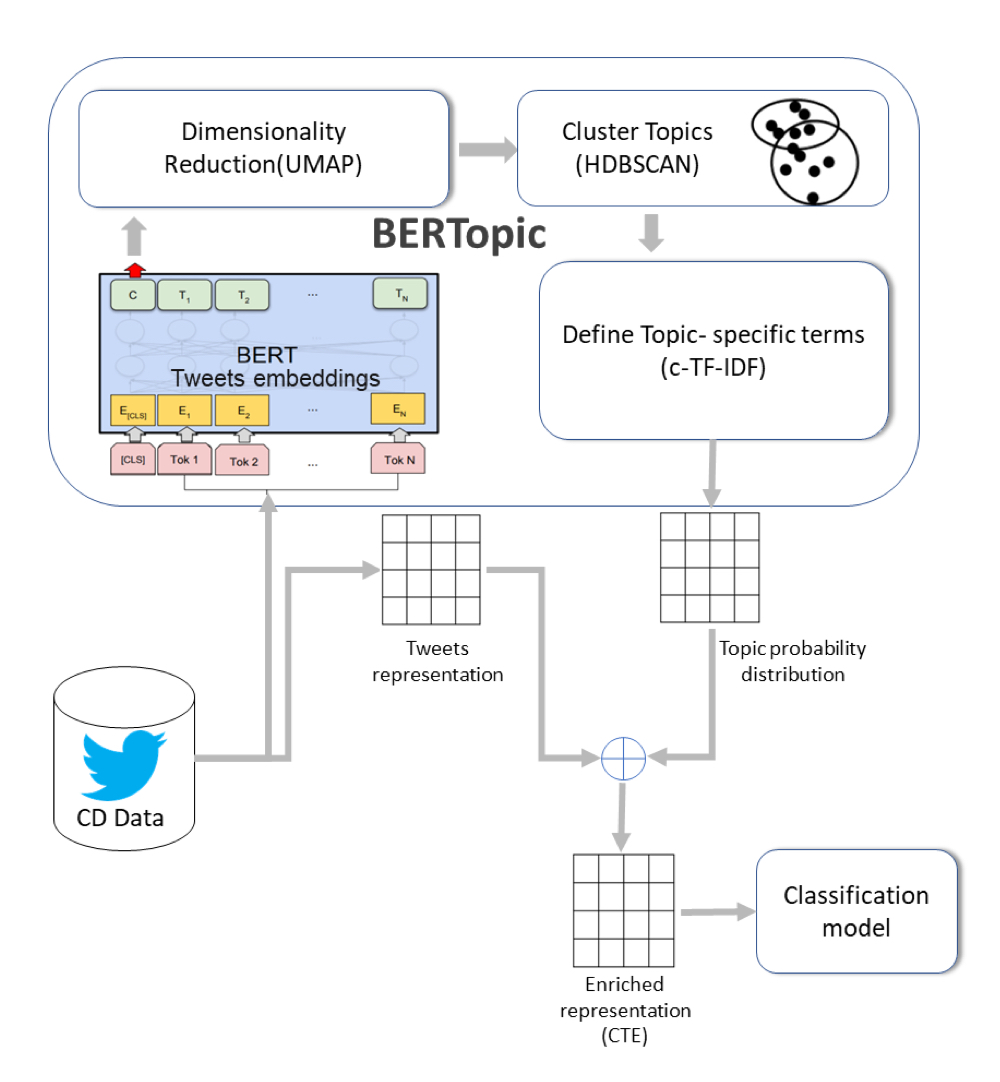
\includegraphics[width=12cm]{grafiken/BERTopic_Word2Vec_TC.jpeg}
\caption[Illustration der Anreicherung von Textrepräsentationen mit Topic Modeling]{Illustration der Anreicherung von Textrepräsentationen mit Topic Modeling aus \textcite[4]{alhaj2022improving}}.
\label{BERTopic_Word2Vec_TC}
\end{center}
\end{figure} 
\noindent Schließlich vergleichen die Autoren die Performanz verschiedener Klassifikatoren auf entweder der nur auf Word2Vec basierenden Tweet-Repräsentation, oder der angereicherten Tweet-Repräsentation aus. Der SVM Klassifikator konnte hierbei (neben der Machine Learning Methode des \textit{Stacking}) besonders gut abschneiden.

\chapter{Exkurs zur Musikgeschichte: Komponisten im Nationalsozialismus} \label{Exkurs}
Der geschichtliche Hintergrund für die beiden Klassen, die vom Textklassifikationsmodell unterschieden werden sollen, ist einerseits das Verbot von als „entartet“ diffamierter Musik im Dritten Reich und andererseits die Förderung und Entlastung bestimmter Personen, die der politischen und ästhetischen Agenda der Nationalsozialisten besser entsprachen.\\
Der Begriff der „Entarteten Musik“ lässt sich auf die gleichnamige Ausstellung im Rahmen der Reichsmusiktage 1938 in Düsseldorf zurückführen, die von Hans Severus Ziegler in Anlehnung an Ausstellung „Entartete Kunst“ aus dem Jahre 1937 initiiert wurde. 
\begin{figure}[H]
\begin{center}

\includegraphics[width=3cm]{grafiken/Entartete_Musik.png}
\caption[Titelbild der 1939 erschienenen Broschüre zur Ausstellung „Entartete Musik“]{Titelbild der 1939 erschienenen Broschüre zur Ausstellung „Entartete Musik“,\\ https://holocaustmusic.ort.org/de/politics-and-propaganda/third-reich/, letzter Zugriff: 12.11.2022 (Screenshot vom 12.11.2022, 21:45 Uhr)}.
\label{bild:verfolgt}
\end{center}
\end{figure}
\noindent Auf dem Titelbild der Broschüre zur Ausstellung (s. Abb. \ref{bild:verfolgt}) wird die Hauptfigur der Oper „Johnny spielt auf“ von Ernst Krenek karikatiert dargestellt und die Jazzmusik als ein Produkt der Vermischung unterschiedlicher Kulturen dargestellt, was dem Gebot der Rassenreinheit der Nationalsozialisten widersprach \parencite{saxophon}.\\ Neben der Jazzmusik wurde die Musik jüdischer Komponisten und atonale Musik abgewertet. 
In seiner Rede zur Eröffnung der Ausstellung sprach Ziegler: 
\begin{quote}Ich bekenne mich mit einer Reihe führender musikalischer Fachmänner und Kulturpolitiker zu der Anschauung, dass die Atonalität als Ergebnis der Zerstörung der Tonalität Entartung und Kunstbolschewismus bedeutet. Da die Atonalität zudem ihre Grundlage in der Harmonielehre des Juden Arnold Schönberg hat, so erkläre ich sie für das Produkt jüdischen Geistes. [...] \\
Wer in die Schule Beethovens geht, kann unmöglich über die Schwelle der Werkstatt Schönbergs finden, wer sich aber länger in dieser Werkstatt Schönbergs aufgehalten hat, verliert notwendigerweise das Gefühl für die Reinheit Beethovens.\\
Aus: \textcite[Rede Hans Severus Zieglers vom 25. Mai 1938, auf CD bereitgestellt vom Deutschen Rundfunkarchiv]{saxophon}\end{quote}
Schon etwa seit März 1933 begann Joseph Goebbels den Kunst- und Kulturbetrieb gleichzuschalten. Die bekannten Komponisten Arnold Schönberg und Franz Schreker wurden im selben Jahr von der Preußischen Akademie der Künste ausgeschlossen. Die Säuberung der Musikszene führte dazu, dass bis Ende 1935 viele jüdische Musiker und Komponisten ins Exil getrieben wurden und meist in den USA, oder in Palästina einen Neuanfang wagten.\\ 
\\
Auf der anderen Seite gab es auch Profiteure des NS-Regimes, wie Carl Orff. Sein bis heute in den Opernhäusern präsentes Werk „Carmina Burana“ ist innerhalb des NS-Regimes entstanden und 1937 in Frankfurt am Main uraufgeführt worden.\\
Jene als „gottbegnadet“ geltende Komponisten, wurden aufgrund ihrer angeblich hohen Bedeutung für die deutsche Identität vom Kriegsdienst befreit.\\ 
\\
Auch das Andenken bereits verstorbener Komponisten wurde angetastet. Beispielsweise konnten die Bayreuther Festspiele, welche von Richard Wagner begründet wurden, vom Nationalsozialismus profitieren, während Stücke des Komponisten Felix Mendelssohn Bartholdy aus den Konzertsälen verschwanden.

\chapter{Methodik} \label{Methodik}
\section{Klassifikation von Texten eines geisteswissenschaftlichen Themas}
Für diese Bachelorarbeit kann das von \textcite{dl_in_dh} genannte Problem der Nicht-Verfügbarkeit von bereits annotierten fachspezifischen Korpora bestätigt werden (s. Kapitel \ref{dl_in_dh}). Daher werden die Annotationen über die von Nutzern durchgeführten Kategorisierungen von Wikipedia-Konzepten und deren Sammlung zu speziellen Listen generiert. Die über diesen Weg vorgenommene Einteilung der Komponisten in die zwei Klassen „begnadet“ und „verfolgt“ bedeutet eine starke Vereinfachung, welche allerdings für das Machine Learning notwendig ist. Es werden in dieser Kategorisierung die vielfältigen Schattierungen innerhalb dieser Klassen außer Acht gelassen, seien die Komponisten Opportunisten, Profiteure oder Mittäter, sowie auf der anderen Seite Ausgeschlossene, Verfolgte oder Ermordete gewesen.\\
\textcite{Kirschenbaum2007TheRO} stellt die gegenteiligen Kulturen der Geisteswissenschaften und der Informatik heraus. Die Geisteswissenschaften pflegten eine von Interpretation, Argumentation und Mehrdeutigkeit geprägte Kommunikationskultur, die eine \textit{ground truth} kaum akzeptieren könne und weniger auf das Problemlösen fokussiert sei \parencite[vgl.][S. 1]{Kirschenbaum2007TheRO}. Die Textklassifikation durch eine Maschine könne in den digitalen Geisteswissenschaften dafür genutzt werden, um neue, unerwartete Erkenntnisse über bekannte Texte zu erlangen und nicht in erster Linie, um einen Experten durch eine Maschine zu ersetzen \parencite{Kirschenbaum2007TheRO}.\\
Es wird daher auch für diese Arbeit angenommen, dass die radikale binäre Klassifikation der Komponisten zu interessanten Ergebnissen führen kann.

\section{Wikipedia als Datenquelle}
Ausschlaggebend für die Entscheidung Wikipedia als Datenquelle zu nutzen ist ihre Mehrsprachigkeit, die es ermöglicht vergleichbare Textkorpora in verschiedenen Sprachen zu erhalten \parencite{wiki_multilingual}. Die Wikipedia ist seit ihrer Gründung im Jahr 2001 eine rasant wachsende und einzigartige Basis für frei zugängliches Wissen und wird damit ihrem Namen gerecht, der als Schachtelwort das Wort „Wiki“ (hawaiisch für „schnell“) mit dem englischen Wort „encyclopedia“ \parencite{wiki:Wikipedia} kombiniert.
Für den Bereich der Natürlichen Sprachverarbeitung in der Informatik können Verlinkungen zwischen Wikipedia-Artikeln und die im Jahr 2004 eingeführten Kategorien zum Beispiel für die Korpuserstellung hilfreich sein. \\
Dabei werden die Kategorienzuordnungen in dieser Bachelorarbeit als Annotationen der Seiten aufgefasst.\\ 
Durch die kollaborative Partizipation mehrerer Autoren an Wikipedia-Artikeln wird bei den annotierten Daten vom \textit{Goldstandard} ausgegangen, d.h. von manuell annotierten Daten, deren Annotation überprüft wurde und gegen die die automatische Klassifikation des Systems gegengeprüft wird \parencite{bird2009natural}. Durch diese Annahme entfällt der aufwändige Schritt der selbst durchgeführten Annotation der Daten, die je nach Domäne, bestimmtes Expertenwissen (hier Wissen im Bereich der Musikgeschichte) voraussetzt.\\ 
Spätestens beim Schritt der Interpretation der Ergebnisse werden allerdings jene Kenntnisse wieder benötigt.\\
Das genaue Vorgehen des Wikipedia Scrapings, sowie die betrachteten Seiten werden in Kapitel \ref{Wiki_scraping} beschrieben.

\section{Textklassifikation mit Word Embeddings und Machine Learning Methoden}
Die Textklassifikation mit statischen Word Embeddings und Machine Learning Algorithmen orientiert sich an der von \textcite{Kowsari_2019} illustrierten Pipeline, deren Schritte im Kapitel \ref{tc_pipeline} des Grundlagenteils vorgestellt wurden.
\subsection{Wahl der Features}
Es stellte sich die Frage, mit welcher Technik die Features für die Machine Learning Modelle generiert werden sollen. Die Wahl fiel auf Word Embeddings (s. Kapitel \ref{Word Embeddings}), da sie in der Literatur schon lange etabliert sind. Die Vorauswahl bestimmter Wörter hätte dazu geführt, dass der Vorteil der Objektivität von automatischen Methoden gegenüber musikwissenschaftlicher Expertenarbeit nivelliert wäre. Daher wurden die Wortvektoren aller Wörter in den Texten verwendet.\\
\\
Ein Dokumentvektor repräsentiert dann den Text eines Dokumentes aus den einzelnen Wortvektoren, die im Vokabular des Embedding Modells nachgeschlagen werden und wird als Feature den Klassifikationsalgorithmen übergeben. Hier als \textit{mean representation vector} definiert, berechnet sich der Dokumentvektor aus dem Durchschnitt aller Wortvektoren im Dokument.\\
\\
Die gewählten Techniken zur Generierung von Words Embeddings waren Word2Vec und fastText. Es wurde mit verschiedenen Ansätzen Word Embeddings zu erhalten experimentiert.\\
Der Ansatz die Word Embeddings selbst zu trainieren wurde verfolgt, um speziell auf die Texte angepasste Embeddings zu erhalten. Der Suchbegriff „Schönberg“ findet in Wikipedia beispielsweise etwa 80 Orte und sehr viele Namensträger. Wir möchten jedoch einen Wortvektor für den Komponisten (Arnold) Schönberg erhalten. Im Grundlagenteil wurde gezeigt, dass statische Word Embeddings nur einen Wortvektor für ein Wort berechnen können. Im genannten Beispiel könnte der Worvektor für „Schönberg“ somit für mehrere Orte, Berge, oder Personen gleichzeitig stehen.\\
Allerdings ist der Datensatz für diese Bachelorarbeit sehr klein (s. Kapitel \ref{Analyse}). Daher werden die selbst trainierten Embeddings mit vortrainierten Embeddings für die Textklassifikation verglichen.
\subsubsection{Word2Vec}
Als Baseline wurden Word2Vec Modelle \textit{from-scratch}, also auf dem eigenen Datensatz von Grund auf neu trainiert. Da keine sprachübergreifenden vortrainierten Word2Vec Embeddings in Deutsch und Englisch gefunden werden konnten, wurden auch für den monolingualen Fall keine vortrainierten Word2Vec Embeddings genutzt.\\
Es wurden aufgrund der kleinen Größe des Datensatzes 100-dimensionale Word2Vec-Embeddings generiert. Im Vergleich dazu haben vortrainierte Word Embeddings meist 300 Dimensionen.
\subsubsection{fastText}
Es wurden 300-dimensionale fastText-Embeddings auf den eigenen Daten trainiert, da die MUSE Bibliothek \parencite{conneau2017word}, die später für das Alignment verwendet wurde, ebenso diese Dimensionen verwendet. Für den Kontext des Wortes wurden immer die fünf Wörter vor und nach dem Wort betrachtet. Es wurden Word Embeddings für alle Wörter im Korpus erstellt, die mindestens zweimal vorkamen.
\subsection{Alignment der fastText-Embeddings}
Abbildung \ref{aligned_articles} illustriert das Vorgehen für das Alignment der monolingualen fastText-Embeddings. Das Alignment von fastText-Embeddings mit MUSE wurde im Grundlagenteil beschrieben (s. \ref{grundlage_muse}). Das Vorgehen orientiert sich an dem Vorgehen von \textcite{jiang2019cross}. Die Autoren haben zum Vergleich auch die Methode der Machine Translation verwendet, die aber in dieser Bachelorarbeit nicht angewendet wurde. 
\begin{figure}[H]
\begin{center}
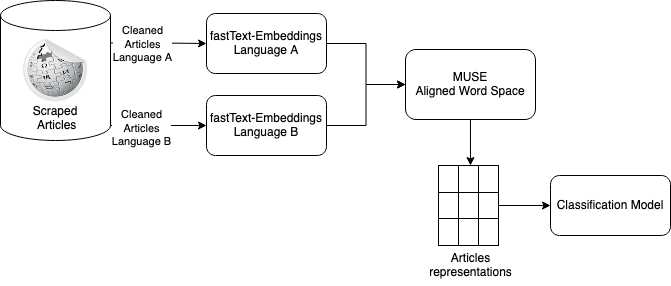
\includegraphics[width=14cm]{grafiken/MUSE_aligned_embeddings.drawio.png}
\caption[Alignment der Word Embeddings]{Alignment der Word Embeddings, eigene Darstellung, angelehnt an \textcite[2]{jiang2019cross}}.
\label{aligned_articles}
\end{center}
\end{figure}

\subsection{Anreicherung der Word Embeddings durch Topic Modeling}
Angelehnt an die Methode von \textcite{alhaj2022improving}, wurden in dieser Arbeit für jeden Artikel die n=3 wahrscheinlichsten Themenwörter des Artikels generiert. Da das BERTopic-Modell auf Sätzen trainiert wurde (s. Kapitel \ref{bertopic_}), musste ein Mapping von den Satz-Thema-Zuordnungen auf den Artikel stattfinden. Die so erhaltenen Topics mit ihren jeweils 10 Themenwörtern wurden dem bereinigten Text angehängt, damit neue Features zu generieren. Die Methode wird in Abbildung \ref{Enriched_articles} beschrieben. 
\begin{figure}[H]
\begin{center}
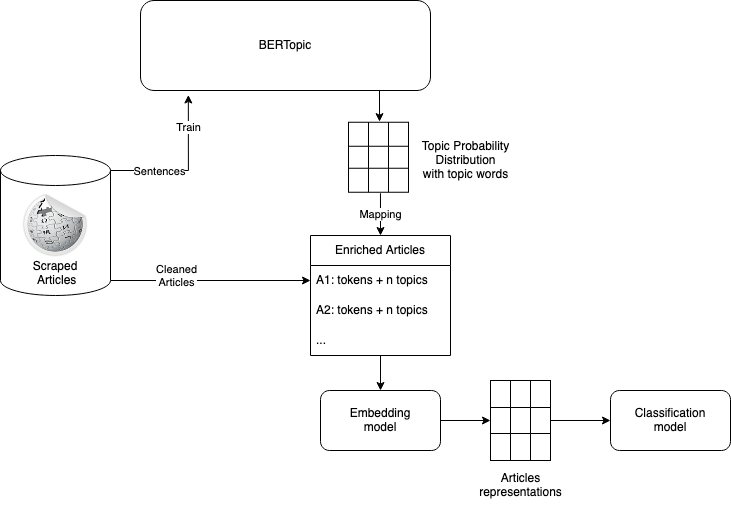
\includegraphics[width=16cm]{grafiken/Topic_Enriched_Articles(1).png}
\caption[Anreicherung von Texten mit Topic Modeling]{Anreicherung von Texten mit Topic Modeling, eigene Darstellung, angelehnt an \textcite[4]{alhaj2022improving}}.
\label{Enriched_articles}
\end{center}
\end{figure}
\subsection{Wahl der Klassifikationsverfahren}
Ein wichtiger Punkt zur Wahl des richtigen Klassifikationsverfahrens ist die Frage, wieviele Daten vorhanden sind \parencite{manning2008introduction}. Generell sei aus der Praxis die Daumenregel entstanden, dass mit einer Verdopplung der Menge der Trainingsdaten die Performanz der Klassifikationsverfahren linear ansteige \parencite{manning2008introduction}. Da eine Korpuserweiterung um vergleichbare biografische Texte von Komponisten in verschiedenen Sprachen für diese Bachelorarbeit nicht möglich ist, kann auch die Zahl der Trainingsdaten auf diesem Weg nicht erhöht werden.

\subsubsection{Naïve Bayes}
Der im Kapitel \ref{NB} beschriebene Naïve Bayes Klassifikator wird in unserem Fall auf die Klassen C={„begnadet“, „verfolgt“} angewendet. Das Problem des Findens der besten Klasse \(c_{best}\) für ein gegebenes Dokument \(\mathbf{d}\) kann daher in folgender Weise formuliert werden: 
\[c_{best} = \operatorname*{argmax}_{c \in \{„begnadet“, „verfolgt“\}} P(c \mid \mathbf{d})\]
Dabei werden die Wahrscheinlichkeiten \(P(c)\) und  \(P(c \mid \mathbf{d})\) aus den Häufigkeiten im Trainingsdatensatz geschätzt.\\
Seine vereinfachten Annahmen (s. Kap. \ref{NB}) machen Naïve Bayes zu einem effizienten Klassifikator \parencite{Kowsari_2019}. Jedoch beschreiben \textcite{ikonomakis} ihn als nicht ideal für die Modellierung von Texten, da er die Relationen zwischen den Features ignoriert. Sprachen werden somit als \textit{bags-of-words} behandelt.
Naïve Bayes wird aufgrund seines Einsatzes als Baseline in vielen Studien zur Textklassifikation angewendet \parencite{ikonomakis}.
\subsubsection{Support Vector Machine}
\textcite{ikonomakis} zufolge erzielt der SVM-Klassifikator für Texte eine sehr gute Precision, aber einen schlechten Recall. Nach \textcite{manning2008introduction} eigne er sich besonders für Probleme mit einer geringen Menge an Trainingsdaten. Daher wurde er für diese Bachelorarbeit verwendet.
\subsubsection{Oversampling von nicht-balancierten Trainingsdaten}
Unausgeglichene Datensätze (\textit{imbalanced data sets}) können für das Machine Learning problematisch sein. Einen Lösungsansatz bietet das \textit{Resampling} von Datensätzen, welches auf das quantitative Angleichen der Klassen ausgerichtet ist.\\ Neben dem \textit{Oversampling} zählt das \textit{Undersampling} zum Resampling. 
Das Resampling der Daten für diese Arbeit hat experimentellen Charakter. Das Ziel war, ein Gefühl über das Potenzial des Resampling auf einem kleinen Datensatz zu erlangen. Daher wurde auf einen Einsatz und Vergleich verschiedener komplexer Techniken verzichtet und einem naiven Ansatz gefolgt.\\
Es wird die \textit{Random Oversampling} Technik genutzt, bei der die Anzahl der Datensätze in der kleineren Klasse an die der größeren Klasse angeglichen wird, indem zufällige Datensätze (\textit{samples}) dupliziert werden. Ebenso wird ihr Gegenstück das \textit{Random Undersampling} implementiert, welches die Klassengrößen durch Reduzierung der Trainingsdaten der größeren Klasse angleicht.\\
Wo beim Undersampling die Gefahr des Informationsverlusts besteht, kann beim Oversampling das Hinzufügen von redundanten Informationen ein Problem darstellen \parencite{Leevy_imbalance}.
\section{Wahl der vortrainierten BERT Modelle} \label{BERT_Modelle}
Wegen der geringen Anzahl an Trainingsdaten wurde der Ansatz gewählt state-of-the-art vortrainierte Sprachmodelle (PLMs) zu verwenden und Finetuning auf der Task der Textklassifikation zu betreiben.\\
Alle der verwendeten Modelle basieren auf der von \textcite{devlin-etal-2019-bert} vorgestellten BERT-Base Architektur. 
\begin{table}[H]
    \centering
    \caption{Das BERT-Base Modell}.
    \begin{tabular}[h]{lrrrr}
    \toprule
    Layer &  Hidden & Attention Heads & Parameter & Techniken für das Training\\ 
    \midrule
    12 & 768 & 12  & 110M & NSP und MLM\\
    \bottomrule
    \end{tabular} 
    \label{BERT_BASE}
\end{table} 
\noindent Es wurden stets Varianten gewählt, welche die Unterschiede zwischen Groß- und Kleinschreibung beachten. Leider ist BERT nur in der Lage Sequenzen von maximal 512 Token (in Englisch etwa 300-400 Wörter) einzulesen, wobei längere Sequenzen gekürzt werden. Kapitel \ref{Analyse} zeigt allerdings, dass die durchschnittliche Wortzahl eines extrahierten Artikels länger ist.\\
Es wurde dennoch entschieden, das Modell auf Artikelebene, und nicht auf Paragraph- oder gar Satzebene zu trainieren, da die Forschungsfrage dieser Arbeit nach den Klassenzuordnungen der Komponisten fragt.
\subsection{Die verwendeten Modelle}
\begin{itemize}
    \item \textit{bert-base-cased}\footnote{https://huggingface.co/bert-base-cased [Letzter Zugriff am 27.11.2022 um 13:02 Uhr]} (im Weiteren frei mit eBERT abgekürzt)
    \item \textit{bert-base-multilingual-cased}\footnote{https://huggingface.co/bert-base-multilingual-cased [Letzter Zugriff am 27.11.2022 um 13:02 Uhr]} (mBERT) 
    \item \textit{bert-base-german-cased}\footnote{https://huggingface.co/bert-base-german-cased [Letzter Zugriff am 27.11.2022 um 13:04 Uhr]} (gBERT)
\end{itemize}
Das für das Finetuning auf dem englischen Datensatz verwendete eBERT wurde neben einem zweiten Korpus auf der bereinigten englischen Wikipedia vortrainiert, wobei Tabellen, Listen und Referenzen der Artikel gefiltert wurden \parencite{devlin-etal-2019-bert}. Dieses Vorgehen wird auch in dieser Bachelorarbeit im Kapitel \ref{Wiki_scraping} gewählt.\\
\\
Das multilinguale mBERT wurde auf der konkatenierten Wikipedia in 104 Sprachen vortrainiert, darunter sind auch die Sprachen Deutsch und Englisch \parencite{bert_multi}.\\
\\
Das deutsche Sprachmodell gBERT wurde von \textcite{gBERT} auf dem deutschen Wikipedia Dump trainiert. Die Entwickler beschreiben ihre Motivation in der unzureichenden Performanz des multilingualen mBERT auf deutschen Texten (s. Abb. \ref{G_vs_M}).
Das Modell wurde dann auf 5 verschiedenen deutschen Datensätzen und den Downstream Tasks \textit{Multiclass Classification}, \textit{Binary Classification}, \textit{Named Entity Recognition} und \textit{Document Classification} evaluiert und mit dem mBERT (s.u.) verglichen \parencite{gBERT}, wobei es in allen Anwendungen eine bessere Performance als mBERT erreichte.
\begin{figure}[H]
\begin{center}
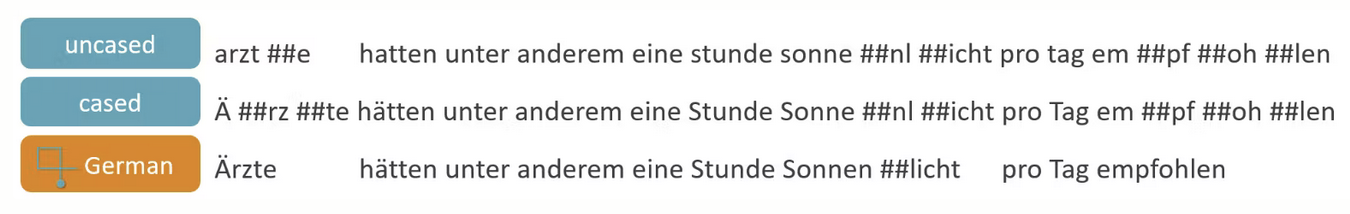
\includegraphics[width=15cm]{grafiken/gBERT.png}
\caption[Limitationen des multilingualen BERT Modells auf einer deutschen Sequenz]{Limitationen des multilingualen BERT Modells auf einer deutschen Sequenz, https://www.deepset.ai/german-bert, letzter Zugriff: 23.11.2022 (Screenshot vom 23.11.2022, 14:54 Uhr)}.
\label{G_vs_M}
\end{center}
\end{figure} 
\subsection{Methodik für das Finetuning}
\textcite{devlin-etal-2019-bert} beschreiben welche Hyperparameter für das Finetuning angepasst werden können. Diese sind Batch-Size, Lernrate und Epochenanzahl. Für das Finetuning werden folgende etablierte Werte vorgeschlagen, welche allerdings für verschiedene Tasks variieren können \parencite[vgl.][13]{devlin-etal-2019-bert}:
\begin{itemize}
    \item Batchgröße: 16, 32
    \item Lernrate des standardmäßigen \textit{Adam}-Optimierers: 5e-5, 3e-5, 2e-5
    \item Epochenzahl: 2, 3, 4
\end{itemize}
Allerdings betonen die Autoren, dass vor allem bei kleinen Datensätze die Hyperparameterwahl sehr große Unterschiede bewirken können und daher viele Kombinationen ausprobiert werden sollten. Der genaue Ablauf des Finetunings wird in Kapitel \ref{TC_BERT} beschrieben.

\chapter{Umsetzung} \label{Umsetzung}
Zunächst werden die in der Implementierung benutzten Frameworks und Bibliotheken im Abschnitt \ref{Implementierung} beschrieben. Der Abschnitt \ref{Daten} befasst sich mit allen Operationen, die zur Vorbereitung des Korpus vorgenommen wurden, beginnend mit der Beschaffung der Texte aus der Wikipedia. Der Aufbau des Kapitels der Textklassifikation mit statischen Embeddings orientiert sich an den Schritten der Pipeline zur Textklassifikation (s. Kapitel \ref{tc_pipeline}) von \textcite{Kowsari_2019}. Danach folgt die Textklassifikation mit BERT.

\section{Verwendete Technologien} \label{Implementierung}
Der Code ist in \textit{Python} (V. 3.9) geschrieben, welches über die Open-Source-Distribution \textit{Anaconda} in der Version 1.9. installiert wurde. Die für diese Arbeit genutzte Entwicklungsumgebung war DataSpell. DataSpell wurde aufgrund seiner Vorteile für die Entwicklung genutzt, darunter Code Completion und Type Hinting. In der browserbasierten Webapplikation \textit{Jupyter Notebooks}, welche im Anaconda-Paket enthalten ist, lassen sich die einzelnen in der Bachelorarbeit vorgenommenen Durchläufe durch angepasste Parameter in den Notebooks steuern, was für die Wiederverwendbarkeit des Codes, aber auch für Code-Demonstrationen vorteilhaft ist. Da das verwendete Betriebssystem MacOs Probleme mit dem Import von den genutzten \textit{spacy} Sprachmodellen aufwarf, wurde Docker genutzt.\\ 
\\
Es wurde ein öffentliches GitHub-Repository für den Programmcode angelegt \parencite{Hassibi_Multi-_und_Monolinguale_2022}.\\
\\
MediaWiki stellt eine API\footnote{https://www.mediawiki.org/wiki/API:Main\_page [Letzter Zugriff am 3. November 2022 um 9:00 Uhr]} für Wikipedia für den freien Zugriff auf Wikipedia-Inhalte bereit. Diese wurde mit dem Wrapper \textit{Wikipedia-API} \parencite{wiki_wrapper} angesprochen.\\
\\
\textit{Pandas} \parencite{mckinney-proc-scipy-2010} erleichterte mit der Datenstruktur \textit{DataFrames} die Operationen auf den Datensätzen, sowie das Lesen und Schreiben der Daten in CSV-Dateien.\\
Des Weiteren wurden \textit{matplotlib} \parencite{Hunter:2007} und \textit{NumPy} \parencite{harris2020array} für die Analyse und Visualisierung der Datensätze genutzt.\\
\\
Die für Tokenisierung und Lemmatisierung genutzte Python Bibliothek war \textit{SpaCy} \parencite{spacy}. Mit SpaCy muss zuerst die Pipelines der jeweiligen Sprachen heruntergeladen und installiert werden. Für Deutsch wurde \textit{de\_core\_news\_sm}\footnote{https://spacy.io/models/de [Letzter Zugriff am 3. November 2022 um 9:15 Uhr]} und für Englisch \textit{en\_core\_web\_sm}\footnote{https://spacy.io/models/en [Letzter Zugriff am 3. November 2022 um 9:15 Uhr]} genutzt.\\
\\
Die Stoppwortlisten für Englisch und Deutsch wurden für diese Arbeit mit \textit{NLTK} \parencite{bird2009natural} geladen. Der Name steht für \textit{Natural Language Processing Toolkit} und für die führende Plattform für Text Processing Bibliotheken und Korpora.\\
\\
Das Topic Modeling wurde mit \textit{BERTopic} \parencite{bertopic} durchgeführt.\\
\\
Die Implementierung und das Training der fastText-Modelle erfolgte mit \textit{gensim} \parencite{rehurek2011gensim}. Das Vector Alignment der fastText-Embeddings wurde mit \textit{MUSE} \parencite{conneau2017word} realisiert.\\
\\
Die vortrainierten BERT Modelle und die zu ihnen passenden Tokenisierer mit der \textit{Huggingface} \parencite{Wolf_Transformers_State-of-the-Art_Natural_2020} Bibliothek geladen.\\
Das Finetuning fand auf einer Tesla T4 GPU in \textit{Google Colab} \parencite{gsuite} statt.\\
\\
Mit \textit{scikit-learn} \parencite{scikit-learn} wurden die SVM- und NB-Klassifikatoren geladen und die Evaluierungen der Textklassifikationen durchgeführt.\\
\\
\textit{Imbalanced-learn} \parencite{imbalanced_learn} ist eine Open Source Python Toolbox, die basierend auf \textit{scikit-learn} Lösungen für die Klassifikation auf unausgeglichenen Datensätzen implementiert und hier das Oversampling ermöglichte.

\section{Daten} \label{Daten}
\subsection{Wikipedia Scraping} \label{Wiki_scraping}
Für die Korpuserstellung wurden zwei deutsche Wikipedia-Seiten betrachtet, welche Auflistungen von Personen beinhalten. \\
Für die Texte, die über die „Gottbegnadeten-Liste“ \parencite{wiki:begnadet} erreicht wurden, wurde das Label „begnadet“ (abgekürzt für „gottbegnadet“) übernommen. Die Texte der „Liste der vom NS-Regime oder seinen Verbündeten verfolgten Komponisten“ \parencite{wiki:verfolgt} bekamen das Label „verfolgt“.\\
Über die Linkstruktur und das Kategoriensystem von Wikipedia konnten die relevanten Seiten extrahiert werden.
\begin{figure}[H]
\begin{center}
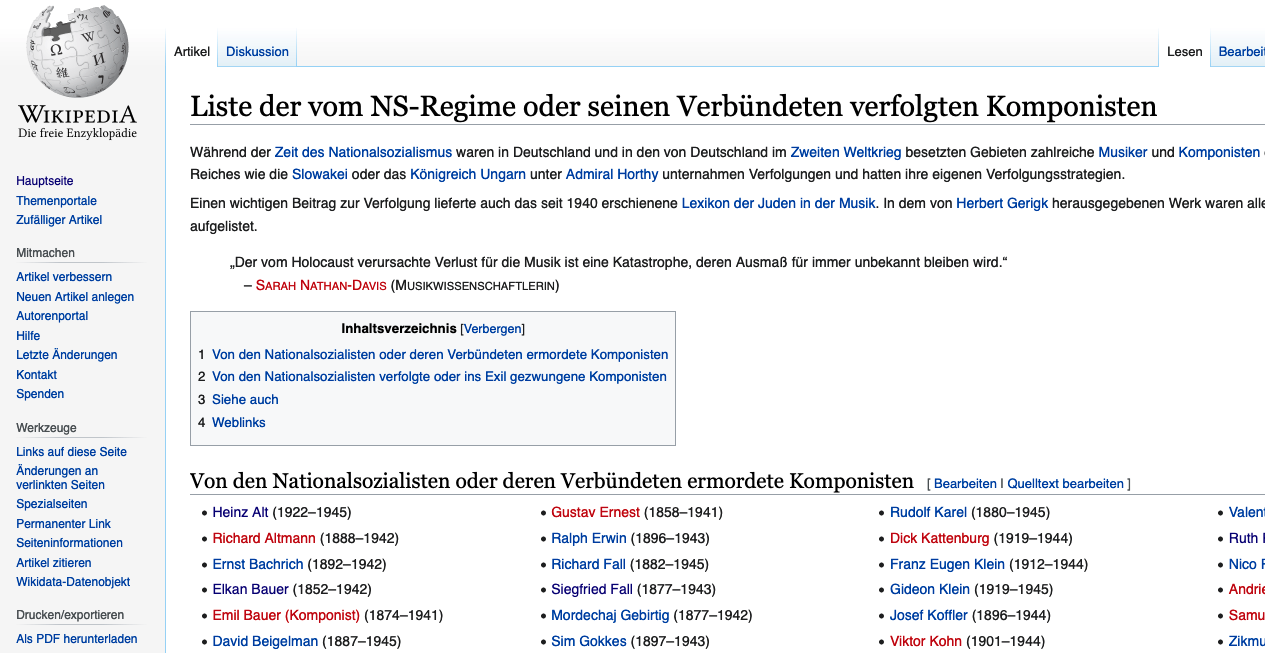
\includegraphics[width=15cm]{grafiken/Wiki_Liste_verfolgt.png}
\caption[Ausschnitt der „Liste der vom NS-Regime oder seinen Verbündeten verfolgten Komponisten“]{Ausschnitt der „Liste der vom NS-Regime oder seinen Verbündeten verfolgten Komponisten“, aus: \textcite{wiki:verfolgt}, letzter Zugriff: 10.11.2022 (Screenshot vom 10.11.2022, 09:20 Uhr)}.
\label{Wikiliste_verfolgt}
\end{center}
\end{figure} 
\subsubsection{Verlinkte Seiten}
Für beide Listen wurde zunächst allen Verlinkungen gefolgt, wobei einige Seiten erreichbar waren, aber keinen Inhalt hatten (in Abbildung \ref{Wikiliste_verfolgt} rot hinterlegte Namen). Diese Fälle wurden abgefangen und verworfen.
\subsubsection{Filtern der Seiten anhand von Kategorien}
Verlinkte Seiten wie „Zeit des Nationalsozialismus“, oder „Musiker“, gehören nicht in den Korpus und sollten ebenso verworfen werden. Daher wurden alle Seiten nach ihren Kategorien abgefragt. Das Filtern nach Kategorien stellte sich allerdings als eine Herausforderung heraus, da die Kategorisierung von Wikipedia-Artikeln eine „Folksonomy“ ist und Wikipedia keine Regeln dafür vorschreibt.\\ 
Zum Beispiel wurde der bekannte Komponist Hanns Eisler sehr detailliert mit insgesamt 24 Kategorien u.a. den folgenden Kategorien zugeordnet: \textit{Komponist klassischer Musik (20. Jahrhundert)} und \textit{Emigrant aus dem Deutschen Reich zur Zeit des Nationalsozialismus}.\\
Der Komponist Walter Jurmann hingegen wurde von den beiden nur der letzten Kategorie zugeordnet, aber daneben in die drei Kategorien \textit{Komponist (Österreich), Filmkomponist, Komponist (Schlager)}.\\ 
Würde nun lediglich nach \textit{Komponist klassischer Musik (20. Jahrhundert)} gefiltert werden, wäre Walter Jurmann verworfen.\\
Um alle Komponisten vollständig zu erfassen, musste also eine Strategie entworfen werden. Im ersten Schritt wurden die Kategorien der Seite abgefragt. Falls das Wort „Komponist“ oder „komponist“ als Teilstring in einer der Kategorien vorkommt, wurde die Seite als „composer“ gelabelt. Falls nicht, wurde die Zusammenfassung der Seite, welche üblicherweise 1-3 Sätze umfasst, aufgerufen und nach dem Wort „Komponist“ abgesucht. \\
Da nun aber auch in anderen musikbezogenen Artikeln das Wort „Komponist“ in der Zusammenfassung vorkommen kann, wurde noch eine letzte Überprüfung durchgeführt. Wurde also das Wort „Komponist“ in der Zusammenfassung des Artikels gefunden, musste versichert werden, dass der Artikel wirklich eine Person beschreibt. Falls eine der Kategorien \textit{Mann, Frau, Person, Geboren, Gestorben} in den Kategorien vorkam, wurde die Seite als „composer“ gelabelt. Ansonsten wurde die Seite verworfen.\\
Nach der Überprüfung aller Verlinkungen der Listen mit dem beschriebenen Verfahren, wurden alle als „composer“ erkannten Artikel in den in der Konfigurationsdatei angegebenen Sprachen aus der Wikipedia gelesen, falls sie in der jeweiligen Sprache existierten. 
\begin{figure}[H]
\begin{center}
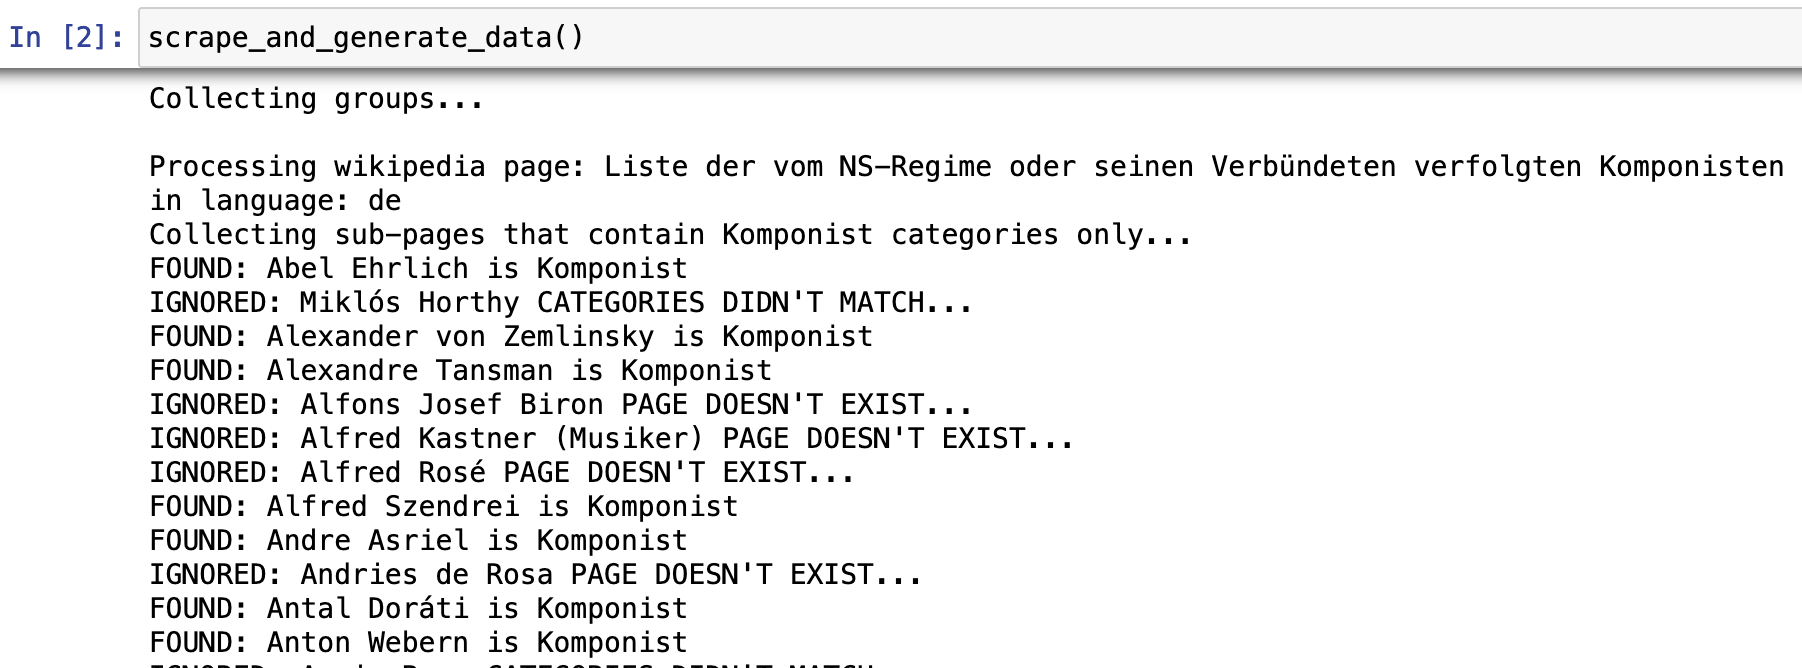
\includegraphics[width=15cm]{grafiken/Data_Scraping.png}
\caption[Konsolenoutput des Data Scrapings  mit Filtern von Komponisten]{Konsolenoutput des Data Scrapings  mit Filtern von Komponisten}.
\label{Data_Scraping}
\end{center}
\end{figure} 

\subsection{Filtern der relevanten Teile der Artikel}
Wikipedia-Artikel über Komponisten beinhalten häufig viele Auflistungen beispielsweise von Werken, oder Ehrungen. Zur Verdeutlichung zeigt Abbildung \ref{Carl_Orff} das Inhaltsverzeichnis der Seite über den Komponisten Carl Orff. Für diese Arbeit relevanter biografischer Text, bestehend aus vollständigen und zusammenhängenden Sätzen, ist nur im ersten Abschnitt „Leben“ und dessen Unterabschnitten vorhanden. Die Abschnitte 2-9 bestehen aus Auflistungen.
\begin{figure}[H]
\begin{center}
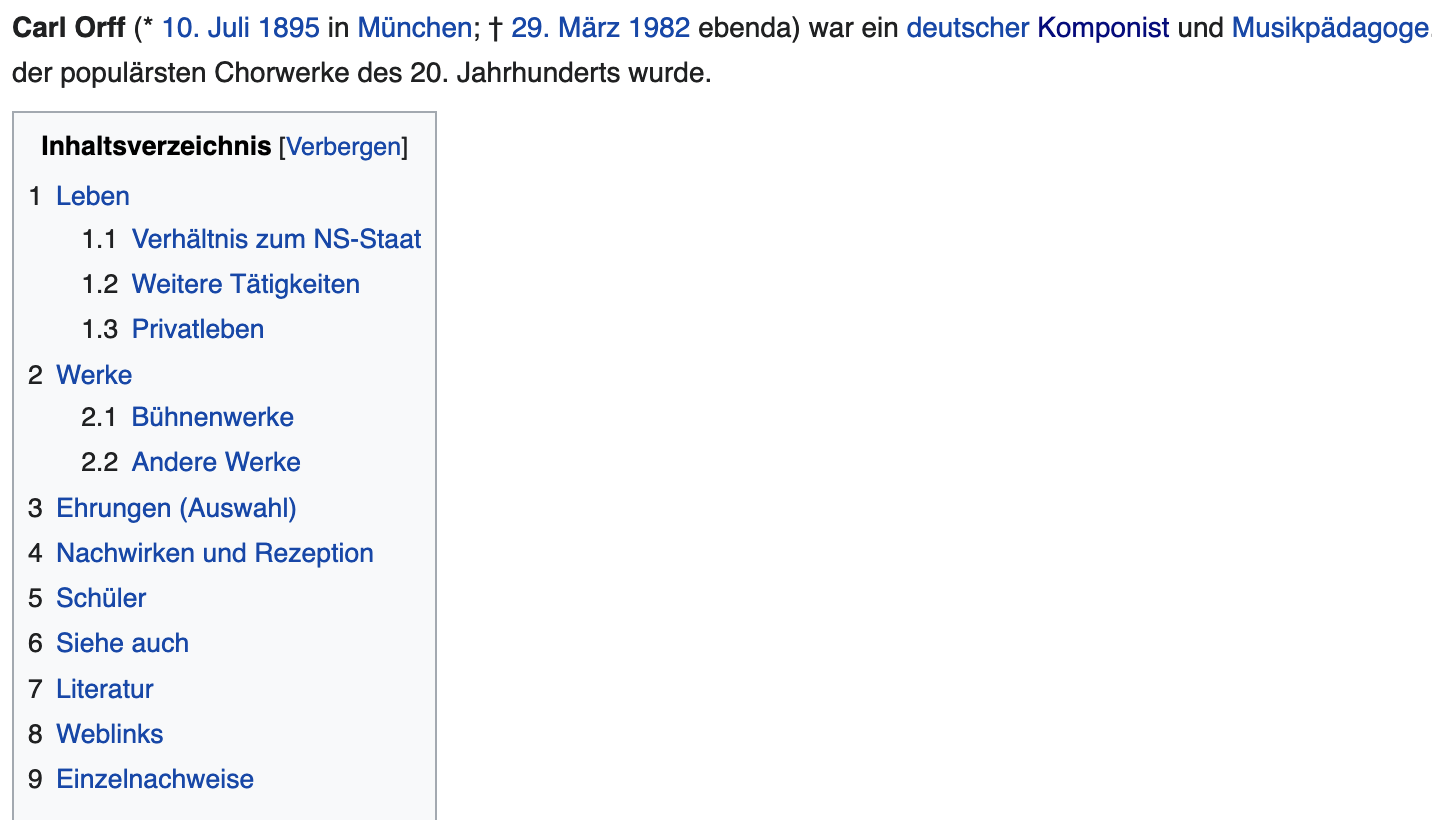
\includegraphics[width=15cm]{grafiken/Carl_Orff_Wiki.png}
\caption[Aufbau des Wikipedia-Artikels über Carl Orff]{Aufbau des Wikipedia-Artikels über Carl Orff,\\ https://de.wikipedia.org/wiki/Carl\_Orff, letzter Zugriff: 10.11.2022 (Screenshot vom 10.11.2022, 10:00 Uhr)}.
\label{Carl_Orff}
\end{center}
\end{figure} 
\noindent Obwohl auch vereinzelt längere Komponisten-Artikel existieren, deren relevanter Text sich über den ersten Abschnitt des Wikipedia-Artikels zieht, musste für das \textit{Wikipedia Scraping} eine allgemeine Lösung entwickelt werden. Daher wurde für alle Artikel lediglich die Zusammenfassung, sowie der erste Hauptabschnitt mit all seinen Unterabschnitten ausgelesen. Da die Unterabschnitte wiederum Unterabschnitte haben konnten, wurde eine rekursive Funktion implementiert, die es ermöglichte den gesamten Text des ersten Abschnitts, mit variabler Ebenenanzahl der Unterabschnitte aufzunehmen.

\subsection{Analyse der Daten} \label{Analyse}
Insgesamt wurden die Texte von \textbf{457} Komponisten-Artikeln mit \textbf{1529} Paragraphen, \textbf{17245} Sätzen und \textbf{276023} Wörtern in sprachspezifische JSON-Dateien geschrieben.\\
\\
Im Anhang A befinden sich die Visualisierungen als Tortendiagramme zu den Sprachverteilungen der extrahierten Artikel, Paragraphen, Sätze und Wörter.\\
\\
Von den 457 Artikeln wurden  376 Artikel mit dem Label „verfolgt“ versehen, und die übrigen 81 Artikel mit dem Label „begnadet“. \\
Die Tabelle \ref{tab:Klassenverteilung} zeigt die Klassen- und Sprachverteilung der Artikel.\\ 
\begin{table}[H]
    \centering
    \caption{Klassen- und Sprachverteilung der Wikipedia-Artikel}.
    \begin{tabular}[h]{lrrr}
    \toprule
    Sprache & \#Artikel &  davon „begnadet“ &  davon „verfolgt“\\
    \midrule
    Deutsch & 266 & 47 & 219 \\
    Englisch & 191 & 34 & 157 \\
    \bottomrule
    \end{tabular} 
    \label{tab:Klassenverteilung}
\end{table} 
\noindent Es wird deutlich, dass das Thema in der deutschen Wikipedia besser dokumentiert ist, trotz größeren Größe der englischen Wikipedia. Außerdem wird ersichtlich, dass es sich um einen unausgeglichenen Datensatz handelt. Tabelle \ref{tab:Scraped_Verteilung} zeigt die durchschnittliche Anzahl der Paragraphen, Sätze und Wörter der extrahierten Datensätze in den verschiedenen Sprachen. 
\begin{table}[H]
    \centering  
    \caption{Durchschnittliche Paragraphen, Sätze und Wörter der extrahierten Datensätze}.
    \begin{tabular}[h]{lrrrr}
    \toprule
    Sprache &  \(\varnothing\) Paragraphen pro Artikel &  \(\varnothing\) Sätze pro Artikel &  \(\varnothing\) Wörter pro Artikel\\
    \midrule
    Deutsch & 2,4 & 32,4 & 487,5 \\
    Englisch & 2,5 & 25,4 & 548,2 \\
    \bottomrule
    \end{tabular} 
    \label{tab:Scraped_Verteilung}
\end{table}
\noindent Die durchschnittlichen Paragraphen, Sätze und Wörter der gesamten Wikipedia-Artikel (nicht nur der extrahierten Textanteile) konnten leider nicht mehr untersucht werden, da das Wikipedia Scraping zum Ende der Bearbeitungszeit immer wieder von der MediaWiki API abgebrochen wurde. In der Fehlermeldung wurden als Grund Wartungsarbeiten angegeben.
\section{Feature Extraction} \label{Feature Extraction}
\subsection{Datenbereinigung und -vorverarbeitung} \label{Datenbereinigung}
Die Datenbereinigung und -vorverarbeitung zählt in der Pipeline von \textcite{Kowsari_2019} zum Teil der \textit{Feature Extraction}. Es wurden folgende Schritte durchgeführt:
\begin{itemize}
    \item Tokenisierung
    \item Lemmatisierung
    \item Entfernung von Stoppwörtern, Punktierungen und Lautschrift
\end{itemize}
\\
Tokenisierung bezeichnet die Segmentierung von Texten in Wörter \parencite{Jurafsky:2009:SLP:1214993}.
In SpaCy muss der Text zunächst in seine Sätze segmentiert werden, bevor auf diese Sätze Tokenisierung angewendet wird.\\
\\
Lemmatisierung bewirkt die Rückführung eines Wortes von seiner flektierten in seine unflektierte Form (auch „Stamm“ oder  „Basisform“ gennant) durch morphologische Analyse des Wortes \parencite{Jurafsky:2009:SLP:1214993}. \\
Beispiele für die Rückführung von Token zu ihren Lemmata sind:\\ 
\textit{sangen} -> \textit{singen} oder \textit{Instrumente} -> \textit{Instrument}.\\
Durch die Lemmatisierung kann die semantische Bedeutung eines Wortes verstärkt werden \parencite{Liu2020}.\\
\\
Als Stoppwörter werden in der NLP Wörter bezeichnet, die in Texten sehr häufig auftreten, aber wenig Inhalt liefern.\\
Punktierungen und Sonderzeichen, die häufig in Wikipedia-Artikeln vorkommen, sollten ebenso aus der Tokenliste entfernt werden. Daher wurde eine Liste dieser Zeichen, bzw. Zeichenkombinationen erstellt. Entfernt wurden:\\
, . ; : (; - – " „  “ / '' "" " ( ) [ ] ! ? = { } \& * † \\
Außerdem sollten auch Namen in phonetischer Schrift entfernt werden, beispielsweise [ˈbeːlɒ:ˈbɒrtoːk"] für den Komponisten Béla Bartók. Dies konnte durch eine selbsterstellte Regex über die Substitutionsfunktion der \textit{re} Bibliothek erreicht werden. 

\subsubsection{Ergebnis}
Nachfolgend wird das Ergebnis der beschriebenen Arbeitsschritte auf zwei Sätze aus Franz Schrekers Biografie aufgezeigt.
\begin{quote}Bereits in den späten 1920er-Jahren war Schreker Angriffsobjekt der Kulturpolitik der Nationalsozialisten. 1932 wurde auf Grund des NS-Terrors die in Freiburg geplante Uraufführung seiner Oper Christophorus von Schreker selbst zurückgezogen, und er wurde zum Rücktritt von seinem Amt als Direktor der Berliner Musikhochschule gezwungen, die er seit 1920 geleitet hatte.\\\parencite{wiki:Schreker}\end{quote}
Ergebnissätze:
\begin{itemize}
\item "`bereits"', "`spät"', "`1920er-Jahr"', "`Schreker"', "`Angriffsobjekt"', "`Kulturpolitik"', "`Nationalsozialist"'
\item "`1932"', "`Grund"', "`NS-Terror"', "`Freiburg"', "`geplant"', "`Uraufführung"', "`Oper"', "`Christophoru"', "`Schreker"', "`zurückziehen"', "`Rücktritt"', "`Amt"', "`Direktor"', "`Berliner"', "`Musikhochschule"', "`zwingen"', "`seit"', "`1920"', "`leiten"'
\end{itemize}

\subsection{MUSE}
Es wurden monolinguale fastText Word Embeddings auf den bereinigten Texten der jeweiligen Sprache trainiert. Auf diesen wurde dann Word Embedding Alignment von der ressourcenreicheren Sprache Deutsch (\textit{source}) auf die ressourcenärmere Sprache Englisch (\textit{target}) durchgeführt. Der Code für die in diesem Abschnitt präsentierten Visualisierungen mit t-SNE stammt aus der MUSE Bibliothek \footnote{https://github.com/facebookresearch/MUSE/blob/main/demo.ipynb [Letzter Zugriff am 26.11.2022 um 9:30 Uhr]}.\\ 
Abbildung \ref{Before_Alignment} zeigt die selbst trainierten monolingualen fastText Wortvektoren im 2-dimensionalen Vektorraum vor dem Alignment.
\begin{figure}[H]
\begin{center}
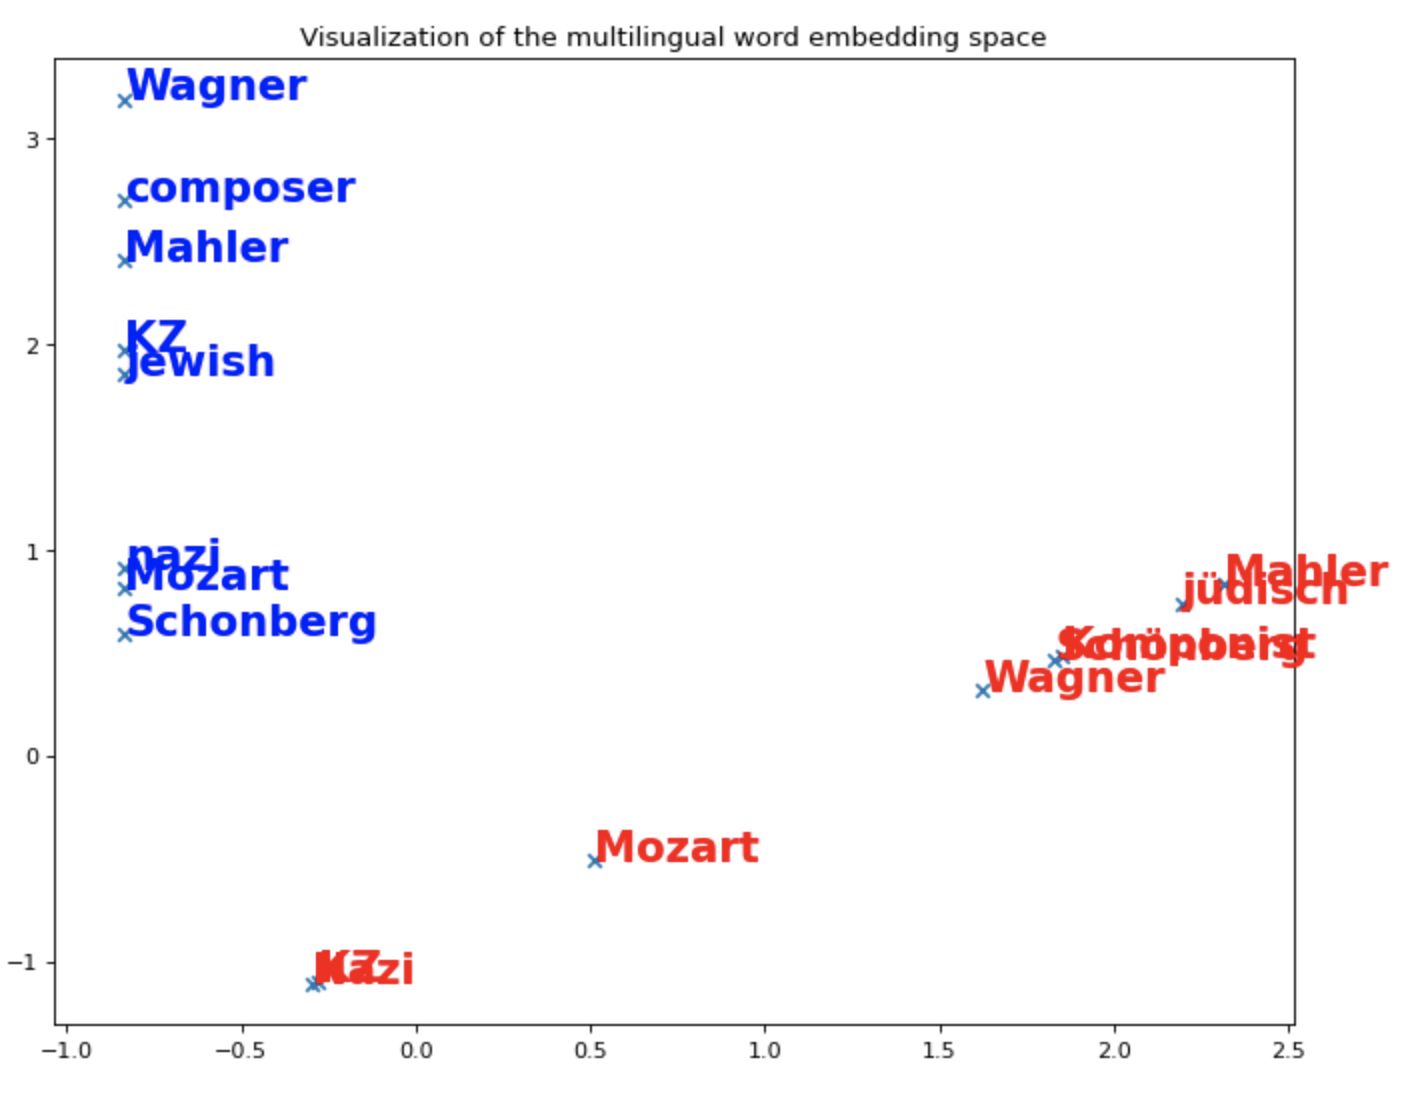
\includegraphics[width=10cm]{grafiken/before_alignment.png}
\caption[Ausgewählte Wortvektoren in Englisch und Deutsch im 2-dimensionalen Vektorraum vor dem Alignment]{Ausgewählte Wortvektoren in Englisch (blau) und Deutsch (rot) im 2-dimensionalen Vektorraum vor dem Alignment}.
\label{Before_Alignment} 
\end{center}
\end{figure} 
\noindent Der Vergleich zu der Abbildung \ref{After_Alignment} nach dem Alignment zeigt, dass der alignierte Wortvektorraum Komponisten sprachübergreifend darstellen kann.
\begin{figure}[H]
\begin{center}
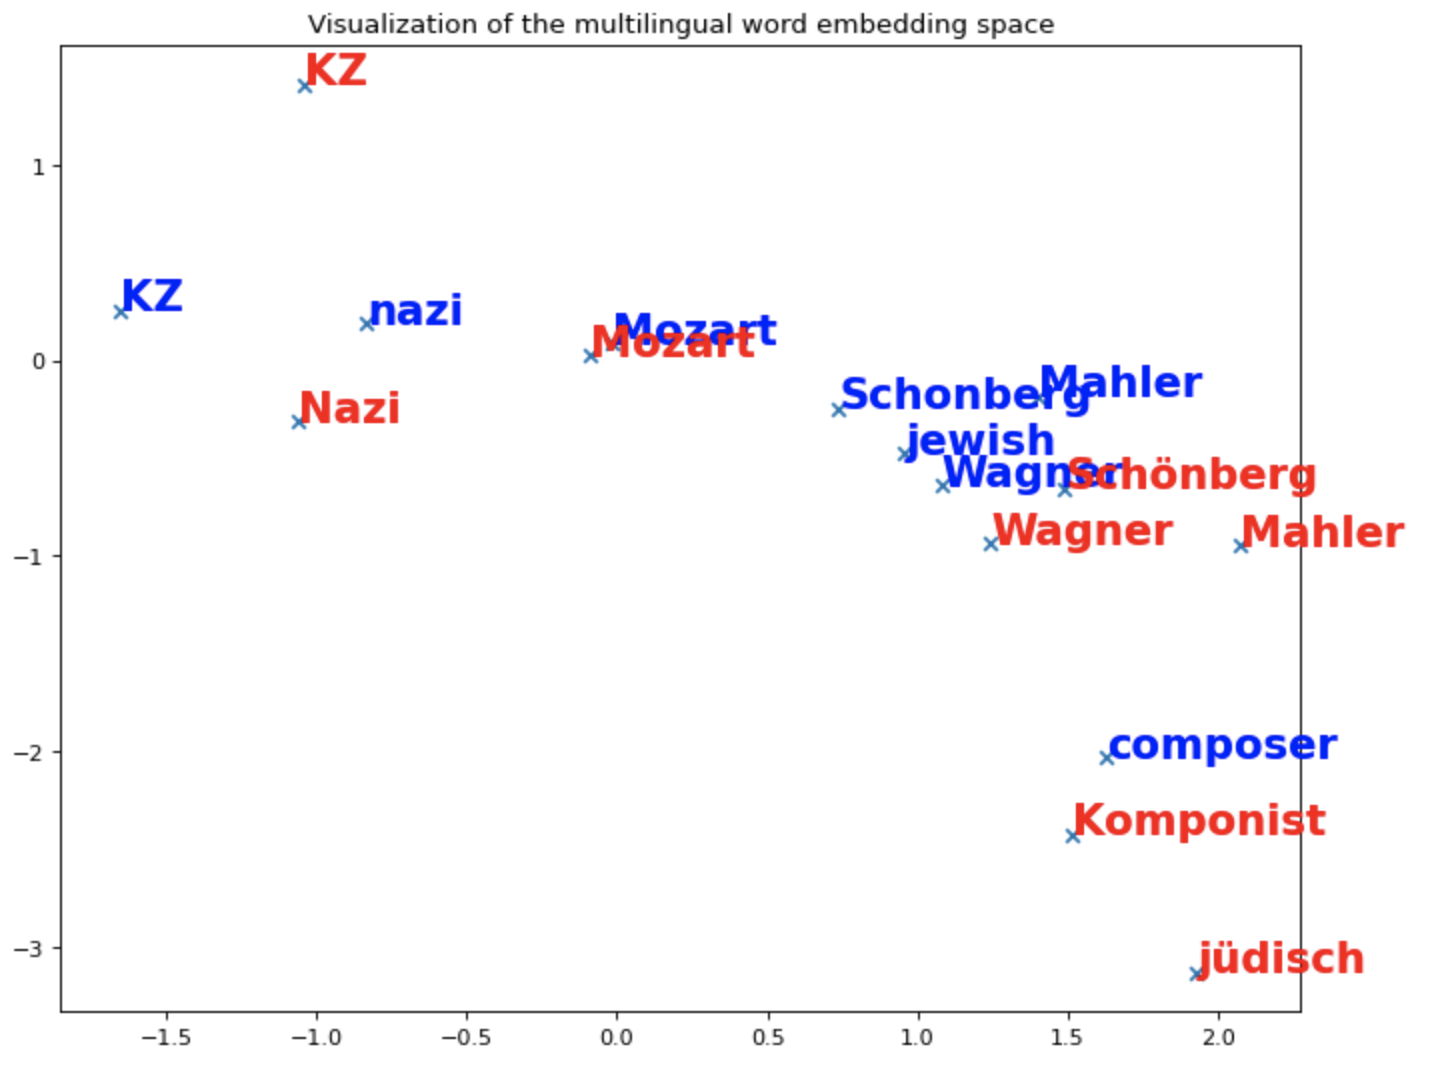
\includegraphics[width=10cm]{grafiken/after_alignment.png}
\caption[Ausgewählte Wortvektoren in Englisch und Deutsch im 2-dimensionalen Vektorraum nach dem Alignment]{Ausgewählte Wortvektoren in Englisch und Deutsch im 2-dimensionalen Vektorraum nach dem Alignment}.
\label{After_Alignment}
\end{center}
\end{figure} 
\noindent Die auf dem Wikipedia Korpus vortrainierten und von \textcite{conneau2017word} im gemeinsamen Vektorraum alignierten Word Embeddings zeigen für die ausgewählten Wörter ebenso gute Ergebnisse (s. Abb. \ref{Pretrained_aligned}). Allerdings wird hier beispielsweise zwischen dem Komponisten Wolfgang Amadeus Mozart und den in dieser Arbeit fokussierten Komponisten kein semantischer Unterschied deutlich. Zudem befand sich der deutsche Wortvektor für Schönberg nicht in der Nähe des englischen, und darüber hinaus nicht in der Nähe der "`Komponistenwolke"'.\\
\begin{figure}[H]
\begin{center}
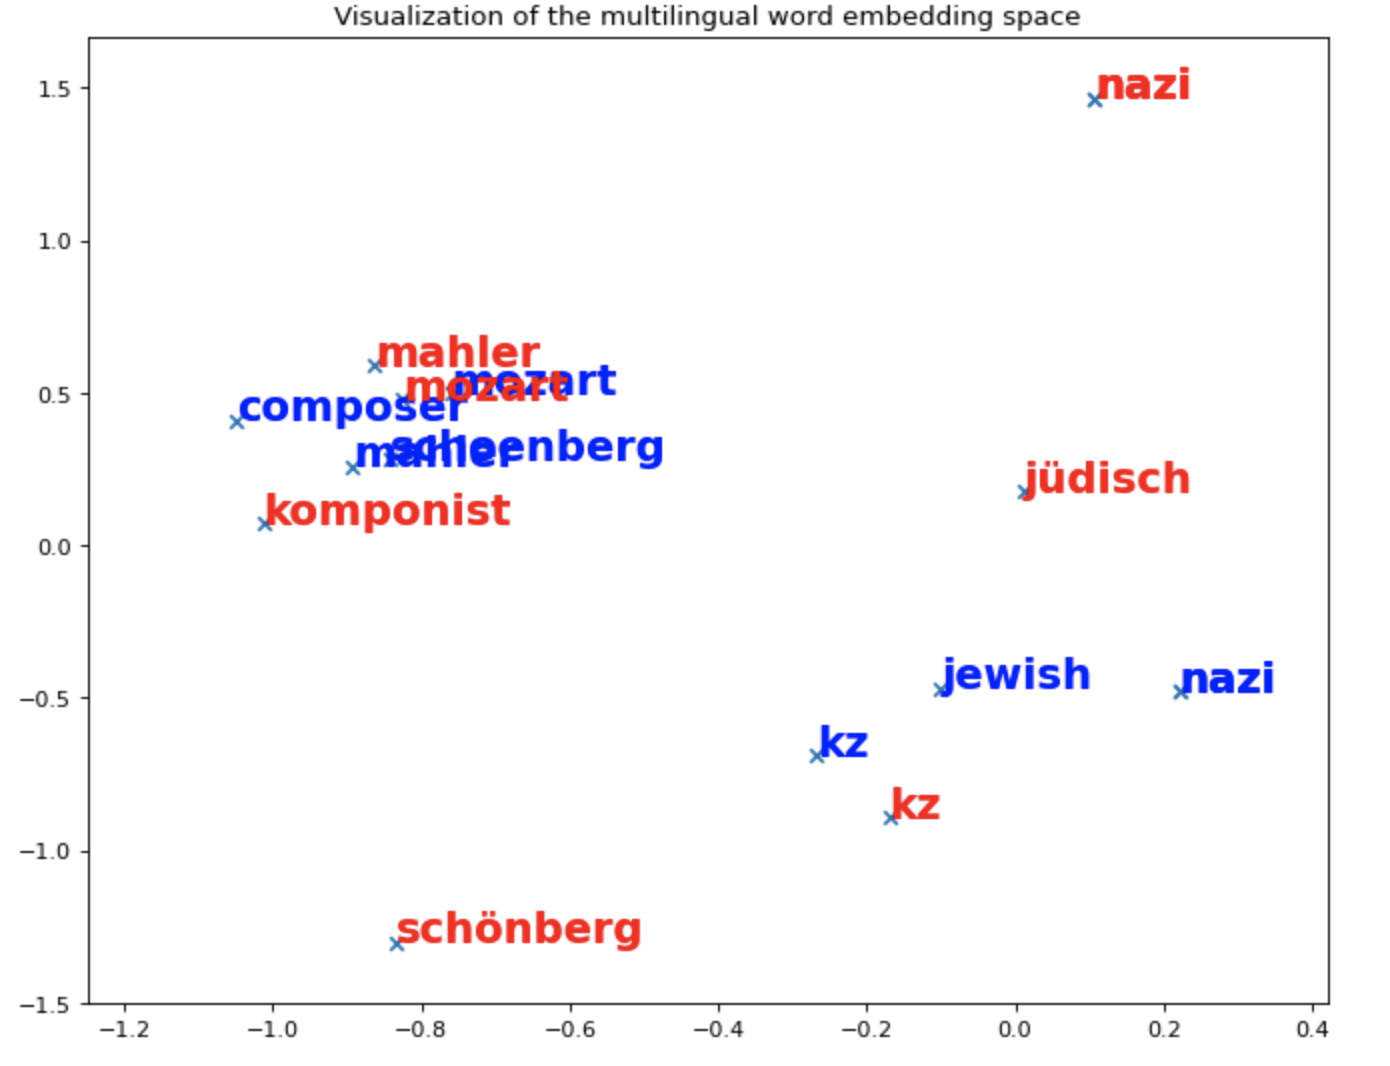
\includegraphics[width=10cm]{grafiken/pretrained_aligned.png}
\caption[Ausgewählte vortrainierte alignierte Wortvektoren in Englisch und Deutsch im 2-dimensionalen Vektorraum]{Ausgewählte vortrainierte alignierte Wortvektoren in Englisch und Deutsch im 2-dimensionalen Vektorraum}.
\label{Pretrained_aligned}
\end{center}
\end{figure}
\noindent Ob die alignierten Word Embeddings analog zu \textcite{jiang2019cross} die Performanz der Textklassifikation erhöhen konnten, wird im Kapitel \ref{Evaluation} besprochen.

\subsection{BERTopic} \label{bertopic_}
BERTopic nimmt eine Liste von Dokumenten, als Eingabe und generiert aus diesen Themenwörtern, die in Clustern ähnlicher Themenwörter zusammengefasst werden (s. Kapitel \ref{Grundlage_Topic_Modeling}).\\
Im Durchlauf des Trainings auf Artikelebene, hat sich herausgestellt, dass keine den vielschichtigen Inhalt eines Artikels angemessen repräsentierende Themen entstehen konnten. Daher wurde entschieden das BERTopic Modell auf Satzebene zu trainieren.\\ 
Für die Embeddings wurden die standardmäßigen Embedding Modelle von BERTopic gewählt, welche Sentence Transformer \parencite{reimers-2019-sentence-bert} für die jeweilige Sprache sind. Für den multilingualen Fall ist dies beispielsweise das multilinguale \textit{paraphrase-multilingual-MiniLM-L12-v2} \footnote{https://www.sbert.net/docs/pretrained\_models.html [Letzter Zugriff am 23.11.2022 um 14:15 Uhr]}.\\
Daher konnte das multilinguale Modell auf den Sätzen aller Sprachen gleichzeitig trainiert werden. Die monolingualen BERTopic-Modelle wurden nur auf den Sätzen der jeweiligen Sprache trainiert.\\ 
Die offizielle Dokumentation von BERTopic empfiehlt, die Texte in ihrer ursprünglichen Form einzugeben und lediglich Stoppwörter zu entfernen. Daher wurden die konkatenierten Stoppwortlisten der verwendeten Sprachen, welche bereits für die Datenvorverarbeitung benutzt wurden, dem BoW-Modell im BERTopic-Algorithmus übergeben. Für den zum Clustern verwendeten UMAP-Algorithmus wurde die minimale Clustergröße 10 definiert.\\
Insgesamt generierte das multilinguale Modell \textbf{285} Topics. Im Anhang B befindet sich eine Liste der 26 häufigsten Topics des multilingualen Modells mit ihren 10 wahrscheinlichsten Topic-Wörtern anhand ihres c-TF-IDF Scores, wobei die meisten die minimale Clustergröße haben und ihre Reihenfolge somit bei wiederholtem Training mit denselben Konfigurationen variiert. Das Topic "`-1"' umfasst Dokumente, die nicht eingeordnet werden konnten, sog. \textit{outliers}. Üblicherweise ist dies das häufigste Topic.
\begin{figure}[H]
\begin{center}
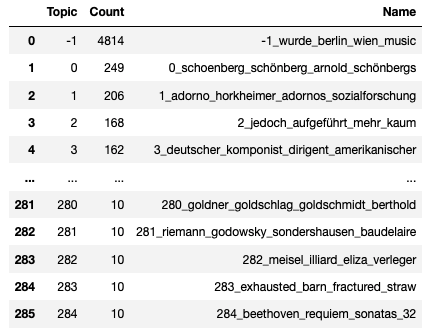
\includegraphics[width=12cm]{grafiken/285_topics.png}
\caption[Generierte Topics und ihre Häufigkeiten des multilingualen BERTopic Modells]{Generierte Topics und ihre Häufigkeiten im des multilingualen BERTopic Modells}.
\label{all_topics} 
\end{center}
\end{figure} 
\noindent Abbildung \ref{most_frequent_topics_de} stellt die 8 häufigsten Topics des deutschen BERTopic Modells in einem Balkendiagramm dar. Im Vergleich zu den Topics des multilingualen Modells (s. Abb \ref{all_topics}) sind Parallelen der gefundenen Topics erkennbar. Beispielsweise ist in beiden Modellen das Thema um den Komponisten Arnold Schönberg wichtig. 
\begin{figure}[H]
\begin{center}
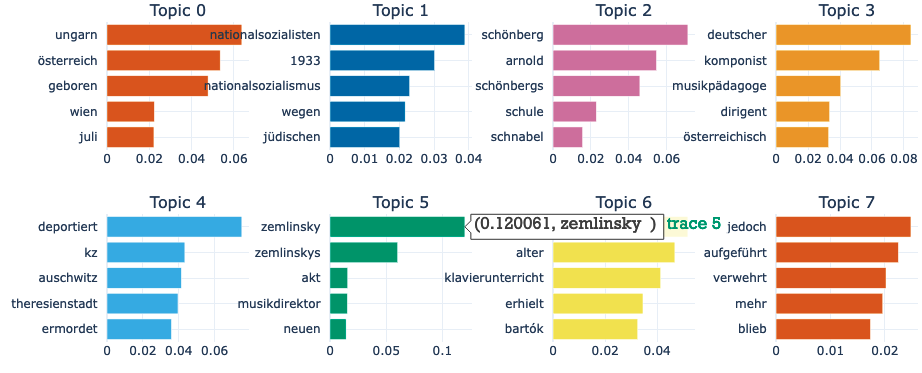
\includegraphics[width=17cm]{grafiken/Topic_word_scores.png}
\caption[c-TF-IDF Scores der 8 häufigsten Topics im deutschen BERTopic Modell]{c-TF-IDF Scores der 8 häufigsten Topics im deutschen BERTopic Modell}.
\label{most_frequent_topics_de}
\end{center}
\end{figure} 
\noindent Zieht man allerdings noch die 8 häufigsten Topics des englischen Modells zum Vergleich hinzu (s. Abb. \ref{most_frequent_topics_en}) ist das Thema um Arnold Schönberg nicht dabei.
\begin{figure}[H]
\begin{center}
\includegraphics[width=17cm]{grafiken/Topic_word_scores_en.png}
\caption[c-TF-IDF Scores der 8 häufigsten Topics im englischen BERTopic Modell]{c-TF-IDF Scores der 8 häufigsten Topics im englischen BERTopic Modell}.
\label{most_frequent_topics_en}
\end{center}
\end{figure} 
\noindent Schönberg scheint dennoch auch in den englischen Artikeln häufig erwähnt worden zu sein, denn im multilingualen Modell ist das Thema auf dem ersten Platz gelandet (s. Abb. \ref{all_topics}).
\subsubsection{Visualisierung der Themenzuordnungen von Sätzen}
BERTopic implementiert eine Methode zur Visualisierung der Themenzuordnungen von Dokumenten im 2-dimensionalen Raum auf Grundlage der gelernten Embeddings des Topic Models. Der so entstandene Plot lässt sich interaktiv durch Herüberfahren mit der Maus (\textit{Hover-Effekt}) nach zugeordneten Dokumenten erkunden. Die nachfolgenden Visualisierungen wurden auf einem multilingualen BERTopic Modell mit den Sprachen Deutsch, Englisch und Französisch erzeugt. Französische Komponistenartikel wurden im Laufe der Bearbeitungszeit verworfen, aufgrund der erhöhten Komplexität des Sprachenvergleichs der Textklassifikation. Dennoch wurden die Screenshots beibehalten, weil sie anschaulich zeigen, dass BERTopic in der Lage war, musikhistorische Zusammenhänge im 2-dimensionalen Raum abzubilden.\\ Es konnten interessante Entdeckungen gemacht werden, beispielsweise in Abbildung \ref{bertopic_sätze}. Dort befindet sich ein Cluster von Sätzen, welches weit entfernt von der „großen schwarzen Wolke“ der Satz-Thema-Zuordnungen befand. Das entfernte Topic lässt sich mit dem Thema „Türkei“ benennen. Ein Beispielsatz handelte von Türkeibesuchen des Komponisten Paul Hindemith und dem großen Respekt, den er bei türkischen Musikern innehatte.
\begin{figure}[H]
\begin{center}
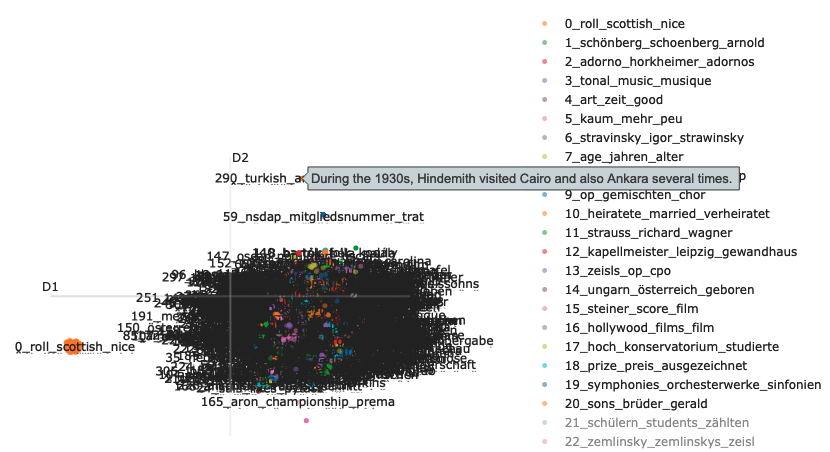
\includegraphics[width=16cm]{grafiken/bertopic_sätze.png}
\caption[Themenzuordnungen der Sätze durch multilinguales Topic Modeling]{Themenzuordnungen der Sätze durch multilinguales Topic Modeling}.
\label{bertopic_sätze}
\end{center}
\end{figure} 
\noindent Durch Auswählen der und „Heranzoomen“ an die Topics, die von Interesse sind, konnten die folgenden Abbildungen \ref{ausgewählte_topics} und \ref{cluster_verfolgt} erstellt werden.
\begin{figure}[H]
\begin{center}
\includegraphics[width=16cm]{grafiken/visualisierung_ausgewählte_topics.png}
\caption[Ausgewählte Topic Cluster im 2-dimensionalem Raum]{Ausgewählte Topic Cluster im 2-dimensionalem Raum}.
\label{ausgewählte_topics}
\end{center}
\end{figure} 
\begin{figure}[H]
\begin{center}
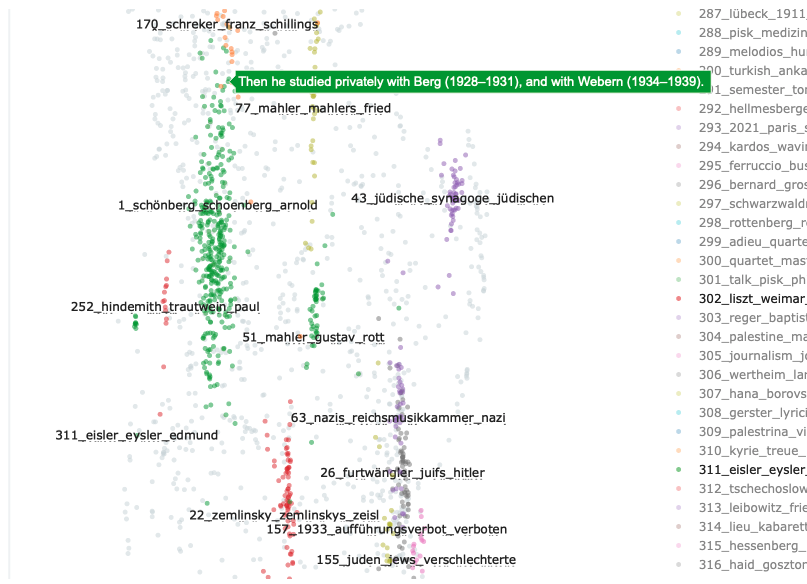
\includegraphics[width=16cm]{grafiken/verfolgte_komponisten_herangezoomt.png}
\caption[Topic Cluster verfolgter Komponisten im 2-dimensionalem Raum]{Topic Cluster verfolgter Komponisten im 2-dimensionalem Raum}.
\label{cluster_verfolgt}
\end{center}
\end{figure} 
\subsection{Training auf um Themenwörter erweiterte Texte} \label{erweiterung_topics}
Mit einer von BERTopic implementierten Methode kann eine Visualisierung der Verteilung der Topics pro Klasse erstellt werden. Es können somit bestimmte Topics ausgewählt werden, von denen erwartet wird, dass sie häufiger in einer bestimmten Klasse auftreten. Dabei waren die meisten Topics aufgrund des Ungleichgewichts der Klassen im Datensatz in der Klasse „verfolgt“ (0) vorzufinden. Es gab jedoch Ausreißer, die häufiger in der Klasse der „gottbegnadeten“ Komponisten vorzufinden waren und aus musikwissenschaftlicher Sichtweise dort auch besser passen.
\begin{figure}[H]
\begin{center}
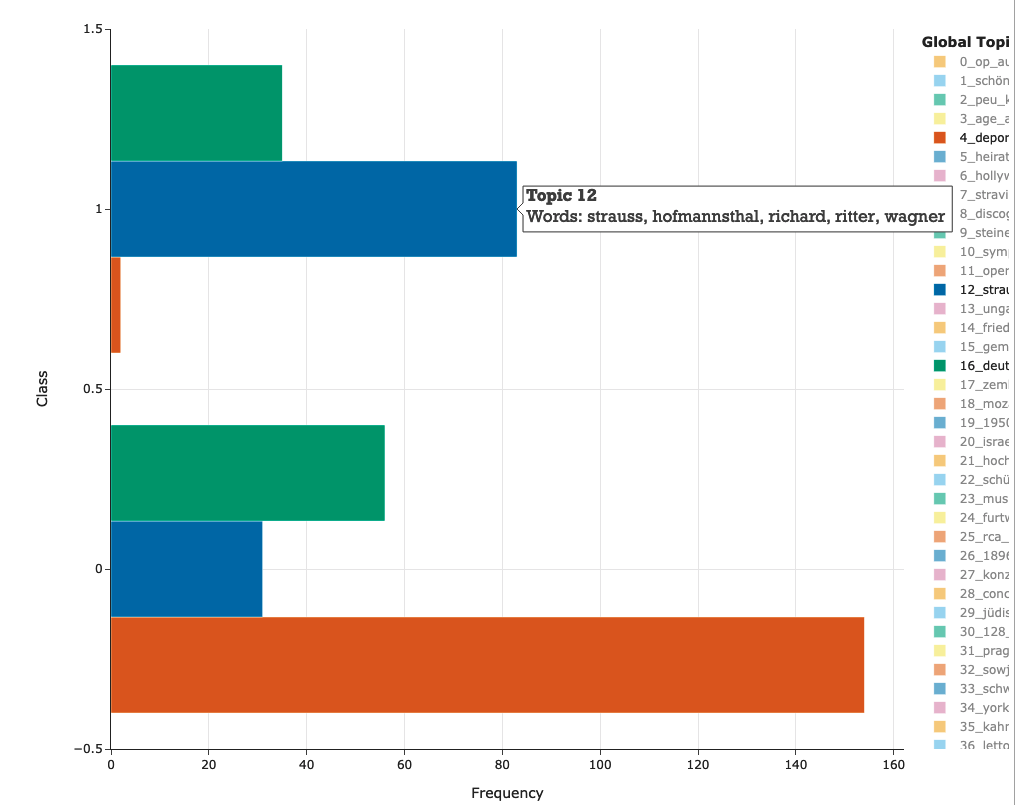
\includegraphics[width=10cm]{grafiken/topics_per_class.png}
\caption[Balkendiagramm der Verteilung ausgewählter Topics pro Klasse]{Balkendiagramm der Verteilung ausgewählter Topics pro Klasse (0=„verfolgt“, 1=„begnadet“)}.
\label{topics_per_class}
\end{center}
\end{figure}
\noindent Daher wurde der Versuch unternommen, die zu einem Text passenden Topics mit ihren Themenwörtern und den bereinigten Text selbst zu konkatenieren. Mithilfe Topic Models, das auf Sätzen trainiert wurde, mussten dafür zunächst die häufigsten Topics den einzelnen Sätzen eines Artikels zugeordnet werden.\\
Es wurden die n=3 wahrscheinlichsten Topics für jeden Artikel abgefragt. Die 10 Topic Wörter eines Topics wurden dann an die Liste der Wörter des bereinigten Artikels gehangen. Das führte zu einer Verlängerung jedes Textes von 30 Wörtern.
\begin{figure}[H]
\begin{center}
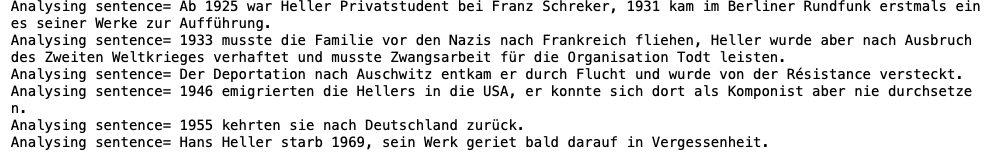
\includegraphics[width=16cm]{grafiken/BERTopic_Satzanalyse.png}
\caption[Konsolenoutput des Mappings von Themen auf Artikel]{Konsolenoutput des Mappings von Themen auf Artikel}.
\label{satzanalyse}
\end{center}
Leider musste festgestellt werden, dass bestimmte Themenwörter sich oft wiederholten, da sie zu besonders häufigen Topics gehörten. In Abbildung \ref{text_topic_dataframe} ist ein Ausschnitt aus der CSV-Datei der bereinigten Datensätze gegeben, der diesen Umstand verdeutlicht. 
\end{figure} 
\begin{figure}[H]
\begin{center}
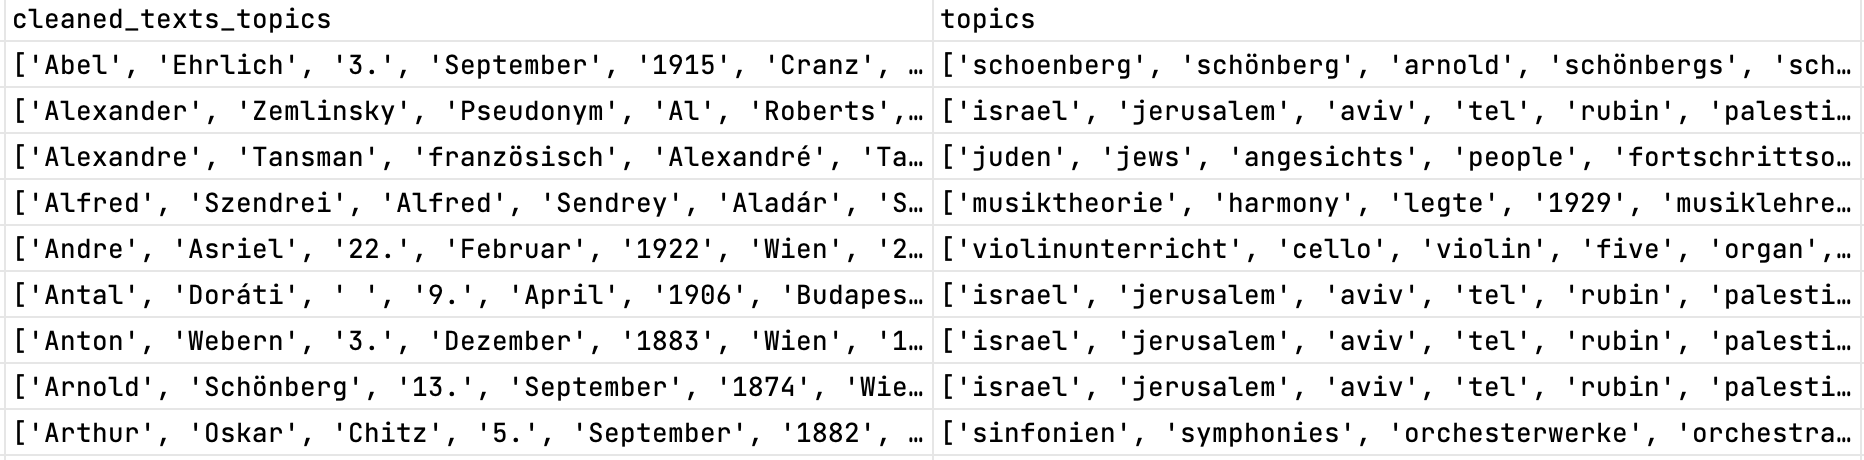
\includegraphics[width=16cm]{grafiken/text_topic_mapping.png}
\caption[Redundanz bestimmter Topics bei Artikeln]{Redundanz bestimmter Topics bei Artikeln}.
\label{text_topic_dataframe}
\end{center}
\end{figure} 
\noindent Auf den so entstandenen Texten wurde dann ebenso eine Variante der Word Embeddings trainiert, die für die Textklassifikation mit dem SVM und Naïve Bayes Klassifikator verwendet werden. 
\subsection{Resampling von nicht-balancierten Trainingsdaten}
Zuletzt wurden aufgrund des Ungleichgewichts der Klassen im Datensatz Resamplingstrategien für die Textklassifikation mit statischen Word Embeddings verwendet.\\ Für die Textklassifikation mit BERT Modellen (siehe nächstes Kapitel) hat dafür die Bearbeitungszeit nicht mehr ausgereicht. Allerdings zeigt Kapitel \ref{Evaluation}, dass die BERT Modelle trotz des unausgeglichenen Datensatzes eine sehr gute Performanz aufwiesen.\\
Die Abbildungen \ref{with_oversampling} und \ref{without_oversampling} veranschaulichen für den Fall des Oversamplings die Distribution der Klassen in den Trainingsdaten des multilingualen Datensatzes vor und nach dem Resampling.
\begin{figure}[H]
\begin{center}
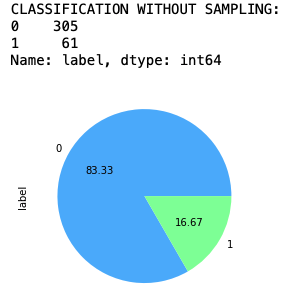
\includegraphics[width=6cm]{grafiken/without_oversampling.png}
\caption[Distribution der Klassen in den Trainingsdaten vor dem Oversampling]{Distribution der Klassen in den Trainingsdaten vor dem Oversampling (0=„verfolgt“, 1=„begnadet“)}.
\label{without_oversampling}
\end{center}
\end{figure} 

\begin{figure}[H]
\begin{center}
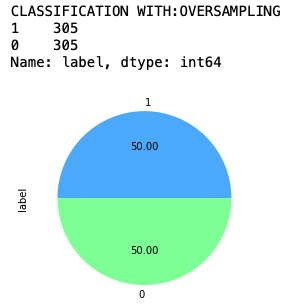
\includegraphics[width=6cm]{grafiken/with_oversampling.png}
\caption[Distribution der Klassen in den Trainingsdaten nach dem Oversampling]{Distribution der Klassen in den Trainingsdaten nach dem Oversampling}.
\label{with_oversampling}
\end{center}
\end{figure}
\newpage
\section{Finetuning von BERT für die Textklassifikation} \label{TC_BERT}
Das Finetuning wurde auf der Task der Textklassifikation betrieben. Dafür wurde der veröffentlichte Code\footnote{https://colab.research.google.com/drive/1IAA1h8u53O1hi9807u7oOFuT3728N0-n?usp=sharing\#scrollTo=hqeWwkSCXaKV [Letzter Zugriff am 27.11.2022 um 08:20 Uhr]} von \textcite{xlm-t} für das Finetuning von XLM-T, einem multilingualen Sprachmodell trainiert auf Twitter Daten, auf den eigenen Anwendungsfall angepasst.\\Die Texte und ihre korrespondierenden Label wurden in Trainings-, Validierungs-  und Testdatensätze eingeteilt. Dabei wurden die unbereinigten Texte als Input ausgewählt, da die gewählten BERT Modelle selbst auf Wikipediatexten trainiert wurde. Da die maximale Sequenzlänge einer Eingabe auf 512 Token beschränkt ist, wurden längere Artikel gekürzt, während kürzere Artikel mit \textit{Padding} versehen wurden. Die notwendigen Tokenisierungsschritte wurden dann vom zum vortrainierten Modell passenden Tokenisierer vorgenommen, der durch die \textit{AutoTokenizer} Klasse von \textit{Huggingface} geladen wurde. 
\begin{figure}[H]
\begin{center}
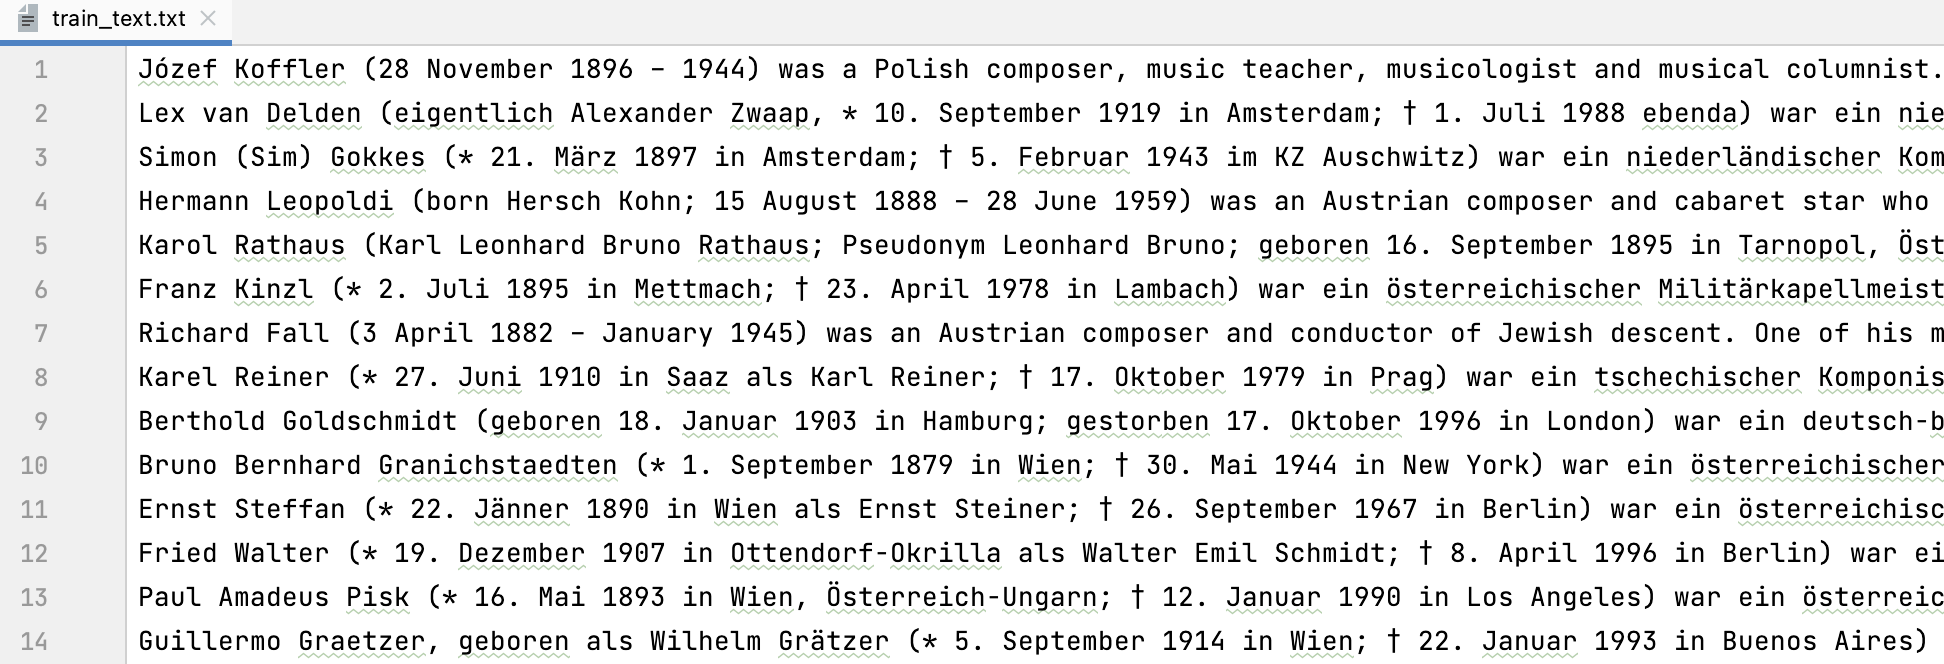
\includegraphics[width=16cm]{grafiken/BERT_X_train_dataset.png}
\caption[Ausschnitt aus dem Trainingsdatensatz für das BERT Modell]{Ausschnitt aus dem Trainingsdatensatz für das BERT Modell}.
\label{BERT_X_train_dataset}
\end{center}
\end{figure} 
\noindent Da die Anzahl der Daten sehr gering ist, war es möglich, mit vielen verschiedenen Hyperparametern zu experimentieren. Es wurden dabei die von \textcite{devlin-etal-2019-bert} angegebenen Hyperparameter für das Finetuning beachtet. Für die Epochenzahl wurden aber teilweise weitaus höhere Epochen ausprobiert, da diese gute Ergebnisse aufzeigten und die Berechnung auf dem Datensatz relativ schnell ging.\\
Es wurde beobachtet, dass eine Erhöhung der Batch-Größe die Accuracy verbesserte. Die Erhöhung der Epochenanzahl führte zu einer höheren Stabilität der Ergebnisse. Allerdings ließ sich nach einer je nach Konfiguration variierender Epochenanzahl beobachten, dass der Loss auf dem Validationsdatensatz wieder anstieg, was auf Overfitting hindeuten könnte. Beispielsweise war das für die Lernrate 5e-5 ab 5 Epochen der Fall.

\chapter{Evaluation} \label{Evaluation}
In diesem Kapitel wird die Güte der verschiedenen Klassifikationsmodelle betrachtet, indem die Vorhersagen der Modelle mit den tatsächlichen Labels verglichen werden.\\
Die für die Evaluation verwendeten Metriken Accuracy, Precision, Recall, und der F1-Score wurden im Grundlagenteil (s. Kapitel \ref{Evaluationsmetriken}) beschrieben. Es werden die Abkürzungen „P“, „R“, „F1“ und „Acc“ verwendet. Sie wurden über die Methode \textit{classification\_report} von scikit.metrics der \textit{scikit-learn} \parencite{scikit-learn} Bibliothek berechnet.\\
Im Folgenden berechneten sich die Werte aus den \textit{macro averages} der jeweiligen Werte für die beiden Klassen, um die Auswirkungen der Unausgeglichenheit des Datensatzes aufzuzeigen. Eine Ausnahme stellt die Accuracy dar, die sich nicht klassenspezifisch verhält, sondern generell die Anzahl der korrekten Vorhersagen unter allen Vorhersagen bemisst.
\section{Ergebnisse der besten Modelle}
Für die Vergleichbarkeit der Ergebnisse wurde für die jeweiligen Durchführungen mit derselben Aufteilung der Datensätze in Trainings-, (Validierungs-), und Testdaten gearbeitet. 
Für beide Ansätze der Textklassifikation wurden umfassende Auswertungen für den deutschen, englischen und den deutsch-englischen Datensatz erstellt, welche sich im Anhang C und D befinden. Die besten Modelle wurden anhand des höchsten  \textit{macro average} F1-Scores bestimmt.
\subsection{Textklassifikation mit Support Vector Machine und Naïve Bayes}
Für die verschiedenen Datensätze wurde die Aufteilung in 80\% Trainings- und 20\% Testdaten vorgenommen. 
In Tabelle \ref{best_ML} werden für jeden Datensatz die besten Textklassifikationen mit Support Vector Machine und Naïve Bayes in einer Tabelle zusammengefasst. Für jeden Datensatz wird jeweils das beste Word2Vec- und das beste fastText-Modell gezeigt, da Word2Vec die \textit{Baseline} darstellt. 
\begin{table}[!ht]
    \centering
    \caption{Performanz der besten Klassifikationsverfahren auf fastText- und Word2Vec-Embeddings} \label{best_ML}
    \begin{tabular}{|l|l|l|l|l|l|l|l|l|}
    \hline
        \textbf{Datensatz} & \textbf{Embeddings} & \textbf{Features} & \textbf{Res.} & \textbf{Klass.} & \textbf{P} & \textbf{R} & \textbf{F1} & \textbf{Acc} \\ \hline
        de & W2V & text & Unders. & NB & 0.59 & 0.56 & 0.49 & 0.50 \\ \hline
        de & fT (p,a) & text & Overs. & SVM & \textbf{0.83} & \textbf{0.77} & \textbf{0.79} &\textbf{0.87} \\ \hline
        en & W2V & text & Overs. & NB & 0.53 & 0.53 & 0.53 & 0.64 \\ \hline
        en & ft (p,a) & text + topics & Overs. & SVM & 0.75 & 0.67 & 0.69 & 0.77 \\ \hline
        de + en & W2V & text + topics & Unders. & NB & 0.61 & 0.56 & 0.51 & 0.59 \\ \hline
        de + en & fT (p,a) & text & Over. & SVM & 0.69 & 0.60 & 0.59 & 0.67 \\ \hline
    \end{tabular}
\end{table}
\newpage \noindent Die beste Textklassifikation fand auf dem deutschen Datensatz mit dem Klassifikationsverfahren Support Vector Machine und nach dem Oversampling statt. Die Features für die SVM waren Dokument-Embeddings ohne Texterweiterung mit BERTopic. Diese wurden mit den von \textcite{conneau2017word} im Vektorraum alignierten vortrainierten fastText-Embeddings (\textit{p,a} für \textit{pretrained} und \textit{aligned}) generiert. 
\subsection{Textklassifikation mit BERT}
Für das Finetuning wurde die Aufteilung der Datensätze in 70\% Trainings-, 15\% Validierungs- und 15\% Testdaten vorgenommen. Auf den monolingualen Datensätzen wurde jeweils ein monolinguales BERT-Modell, als auch ein multilinguales BERT-Modell verwendet. Auf dem multilingualen Datensatz fand das Finetuning nur mit einem multilingualen Modell statt. Tabelle \ref{best_BERT} stellt für jeden Datensatz das jeweils beste der verwendeten Modelle dar.
\begin{table}[H]
    \centering
    \caption{Konfiguration und Performanz der besten der jeweils verwendeten BERT Modelle auf den Datensätzen} \label{best_BERT}
    \begin{tabular}{|l|l|l|l|l|l|l|l|l|l|}
    \hline
        \textbf{Datensatz} & \textbf{Modell} & \textbf{Epochen} & \textbf{Batchgröße} & \textbf{Lernrate} & \textbf{Loss} & \textbf{P} & \textbf{R} & \textbf{F1} & \textbf{Acc} \\ \hline
        de & gBERT & 5 & 16 & 5,00E-05 & 0.35 & \textbf{0.98} & 0.94 & \textbf{0.96} & \textbf{0.97} \\ \hline
        de & mBERT & 20 & 16 & 5,00E-05 & 0.13 & 0.85 & 0.90 & 0.87 & 0.90 \\ \hline
        en & eBERT & 20 & 8 & 3,00E-05 & 0.11 & 0.75 & 0.96 & 0.81 & 0.93 \\ \hline
        en & mBERT & 5 & 8 & 3,00E-05 & 0.46 & 0.73 & 0.73 & 0.73 & 0.93 \\ \hline
        de + en & mBERT & 5 & 16 & 3,00E-05 & 0.46 & 0.93 & \textbf{0.98} & \textbf{0.96} & \textbf{0.97} \\ \hline
    \end{tabular}
\end{table}
\noindent Auf dem deutschen Datensatz konnte \textit{bert-base-german-cased} (gBERT) dieselben besten Werte für Accuracy und F1-Score wie \textit{bert-base-multilingual-cased} (mBERT) auf dem multilingualen Datensatz erreichen. Der höchste Wert für die Precision ist in der deutschen, während der höchste Wert für den Recall in der multilingualen Textklassifikation ist.
\section{Reflexion}
Im direkten Vergleich der beiden Varianten die Textklassifikation durchzuführen wird deutlich, dass das Finetuning von BERT auf der Task der Textklassifikation für alle Datensätze in einer viel höheren Performanz resultiert.
\subsection{Reflexion der Textklassifikationen mit SVM und NB}
Die beste deutsche, englische und deutsch-englische Textklassifikation nutzte stets den SVM-Klassifikator, was sich vielleicht auf die von \textcite{manning2008introduction} erwähnte Eigenschaft der SVM zurückführen lässt, gut auf kleinen Datensätzen zu funktionieren. Wie von den Autoren prophezeit, war die Precision dieses Klassifikators wesentlich höher als der Recall. In den Klassifikationen mit NB war der Unterschied zwischen Precision und Recall wesentlich geringer.\\
Obwohl die besten Textklassifikationen mit SVM und NB stets auf vortrainierten alignierten fastText-Embeddings verliefen, kann nicht sicher gesagt werden, ob der Umstand, dass sie im gemeinsamen Vektorraum angeglichen waren, für dieses gute Ergebnis sorgten. Das liegt daran, dass nicht zusätzlich vortrainierte monolinguale fastText-Embeddings in den Vergleich mit einbezogen wurden. Der Blick in die Tabellen im Anhang C zeigt, dass die vortrainierten und von \textcite{conneau2017word} im gemeinsamen Vektorraum angeglichenen Word Embeddings stets besser F1-Werte erzielten, als die auf den Datensätzen der Bachelorarbeit trainierten und dann mit MUSE alignierten fastText Vektoren (in den Tabellen mit \textit{fT (a)} notiert).\\
Die gute Performanz von fT (p,a) scheint daher eher an der Eigenschaft der Vektoren zu liegen, umfangreich auf der Wikipedia vortrainiert zu sein, was sich insbesondere gut auf die zu klassifizierenden Texte dieser Bachelorarbeit auszuwirken scheint, die ebenso aus der Wikipedia stammen.\\
Bessere Ergebnisse durch linear transformierte fastText, bzw. MUSE-Vektoren, aufgrund der Tatsache, dass sie einen gemeinsamen Vektorraum teilen, analog zu den Ergebnissen von \textcite{jiang2019cross}, konnten daher nicht beobachtet werden.
\\
Des Weiteren zeigt Tabelle \ref{best_ML}, dass die Techniken Oversampling und Undersampling für den F1-Score förderlich waren, da sie der kleineren Klasse der „gottbegnadeten“ Komponisten zu Gute kam.\\ 
Es kann insgesamt für die Textklassifikation mit den Machine Learning Algorithmen SVM und NB gesagt werden, dass sie ausreichend gut funktionierte, wenn man nur die größere Klasse „verfolgt“ mit hoher Sicherheit vorhersagen möchte. Wenn beide Klassen gleichermaßen wichtig waren, wie in dieser Evaluation, waren die Ergebnisse sehr von dem Vorkommen des Labels „begnadet“ im Testdatensatz abhängig.\\
fastText zeigte in fast allen Fällen eine bessere Performanz als Word2Vec und insbesondere basieren die besten Textklassifikationen unabhängig von der Sprache der Datensätze immer auf fastText-Embeddings. Der Grund dafür wird in der Eigenschaft von fastText vermutet, die Morphologie einer Sprache besser als Word2Vec und zudem \textit{Out-of-Vocabulary-Words} modellieren zu können (s. Kapitel \ref{fT_grundlage} in den Grundlagen).
\\
Letztlich konnte keine klare Tendenz zu besseren Ergebnissen durch die Kombination von BERTopic und Word Embeddings wie bei \textcite{alhaj2022improving} beobachtet werden. Zumindest nicht mit der für diese Bachelorarbeit adaptierten Methode, die die Texte um ihre wahrscheinlichsten Themenwörter erweiterte.
\subsection{Reflexion der Textklassifikation mit BERT}
In der Tabelle \ref{best_BERT} für die besten Textklassifikationen mit BERT ist erkennbar, dass auf den monolingualen Datensätzen die monolingualen Modelle besser als das multilinguale BERT-Modell abschneiden. Diese Beobachtung deckt sich mit den Ergebnissen von  \textcite{mono_vs_multi_BERT} und \textcite{gBERT}.\\
Anhand der Tabelle der besten Modelle lässt sich keine optimale Konfiguration der BERT-Modelle feststellen. Es könnte aber argumentiert werden, dass die beiden besten Modelle beide im Finetuning mit 5 Epochen und einer Batchgröße von 16 trainiert wurden.\\
In den Tabellen für den englischen Datensatz in Anhang D zeigt sich, dass sich die Performanz relativ schnell „eingefahren“ hat auf P=0.47, R=0.50, F1=0.48 und Acc=0.93, da das Modell nicht in der Lage war, Komponisten der kleinen Klasse „begnadet“ korrekt zu bestimmen. Dies änderte sich aber beim monolingualen \textit{bert-base-cased}-Modell mit 20 Epochen. Es wäre auch für die Textklassifikation mit BERT und besonders für den englischen Datensatz eventuell vorteilhaft gewesen das Oversampling anzuwenden. Jedoch ließ sich das in Anbetracht der verfügbaren Bearbeitungszeit nicht mehr realisieren.
\section{Musikwissenschaftliches Abfragen des besten Modells}
Im Folgenden wurden interessengeleitet ausgewählte Passagen von Wikipedia-Artikeln über Komponisten kopiert und dem besten multilingualen BERT Modell als Input übergeben. Es wurde darauf geachtet, dass sowohl der Name des Komponisten, als auch ein repräsentativer Satz über dessen Beziehung zum Nationalsozialismus im Text vorkam.\\
Es steht immer das mit höchster Wahrscheinlichkeit vorhergesagte Label an erster Stelle.
\begin{figure}[H]
\begin{center}
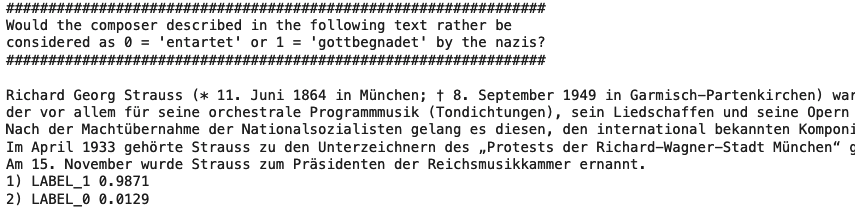
\includegraphics[width=16cm]{grafiken/Abfrage_Strauss.png}
\caption[Abfragen des besten Modells nach der Klassenzugehörigkeit des „gottbegnadeten“ Richard Strauss]{Abfragen des besten Modells nach der Klassenzugehörigkeit des „gottbegnadeten“ Richard Strauss}.
\label{strauss_abfrage}
\end{center}
\end{figure}
\noindent Obwohl Richard Strauss aus der „Gottbegnadeten-Liste“ stammt, aus welcher weniger Datensätze generiert wurden, hat das Modell mit einer sehr hohen Gewissheit die richtige Klasse vorhergesagt (s. Abb. \ref{strauss_abfrage}).
\begin{figure}[H]
\begin{center}
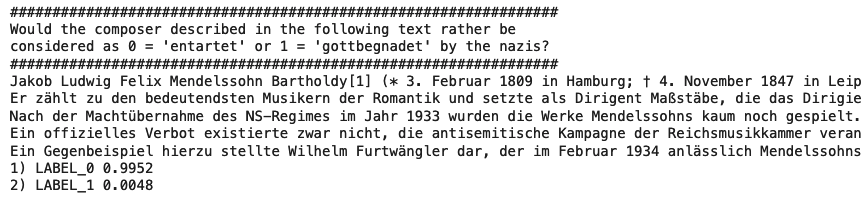
\includegraphics[width=16cm]{grafiken/Abfrage_Mendelssohn.png}
\caption[Abfrage des besten Modells nach der Klassenzugehörigkeit des ungesehenen Felix Mendelssohn Bartholdy]{Abfrage des besten Modells nach der Klassenzugehörigkeit des ungesehenen Felix Mendelssohn Bartholdy}.
\label{mendelssohn_abfrage}
\end{center}
\end{figure}
\noindent Der Komponist Felix Mendelssohn Bartholdy aus der Abfrage in Abbildung \ref{mendelssohn_abfrage} war nicht im Datensatz vorhanden, da er nicht in der Zeit des Nationalsozialismus gelebt hat. Obwohl er zu Lebzeiten eine große internationale Karriere hinlegte, wurde sein Andenken von den Nationalsozialisten geschmäht, weil er Jude war. Das Modell war in der Lage, auf Grundlage des übergebenen Textes die Entscheidung zu treffen, dass Mendelssohn von den Nationalsozialisten als „entartet“ eingestuft worden wäre.\\
\\
Wenn über das Verhältnis von Komponisten zum Antisemitismus gesprochen wird, muss auch Richard Wagner erwähnt werden, der mit seiner Schrift „Das Judenthum in der Musik“ aus dem Jahre 1850 das angeblich Jüdische in der Musik aufs Übelste beschimpfte und dessen Musik von Adolf Hitler vergöttert wurde.\\
Zunächst war die Klassenentscheidung des Modells auf einer Beispielpassage über Richard Wagner enttäuschend, da das Resultat „entartet“ war (s. Abb. \ref{wagner_abfrage}).
\begin{figure}[H]
\begin{center}
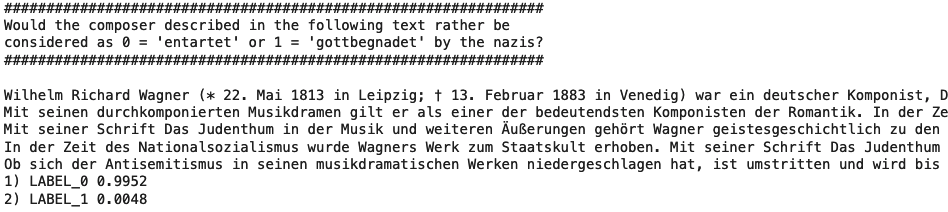
\includegraphics[width=16cm]{grafiken/Abfrage_Wagner.png}
\caption[Abfragen des besten Modells nach der Klassenzugehörigkeit des ungesehenen Richard Wagner]{Abfragen des besten Modells nach der Klassenzugehörigkeit des ungesehenen Richard Wagner}.
\label{wagner_abfrage}
\end{center}
\end{figure}
\noindent Dann fiel auf, dass im Text die Wörter „Antisemitismus“, „Judentum“ und „jüdisch“ vorkamen. Es war zu vermuten, dass das Modell aufgrund dieser Wörter die Klassenentscheidung getroffen hat.\\
Daher wurde ein neuer Abschnitt der Biografie Richard Wagners in der Wikipedia kopiert, welcher u.a. von Wagners Beschäftigung mit germanischer Mythologie handelte. Nun entschied das Modell die entgegengesetzte Klasse (s. Abb. \ref{wagner_abfrage2}).
\begin{figure}[H]
\begin{center}
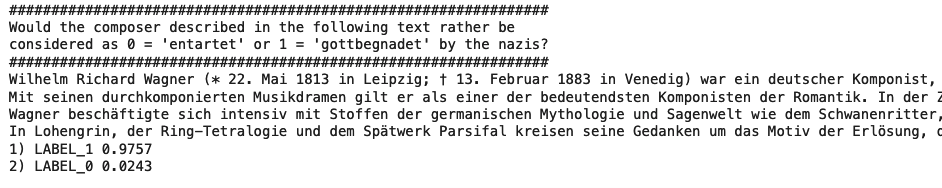
\includegraphics[width=16cm]{grafiken/Abfrage_Wagner2.png}
\caption[Veränderter Input in der Abfrage des besten Modells nach Richard Wagner]{Veränderter Input in der Abfrage des besten Modells nach Richard Wagner}.
\label{wagner_abfrage2}
\end{center}
\end{figure}

\chapter{Schlussfolgerungen und Ausblick} \label{Schluss}
In dieser Bachelorarbeit konnte gezeigt werden, dass es möglich ist, ein Klassifikationsmodell zu trainieren, das in der Lage ist, die „Klassenzugehörigkeit“ eines Komponisten gemäß nationalsozialistischer Denkweise zu bestimmen.\\
Durch das Scraping von Wikipedia-Artikeln zu „gottbegnadeten“ und „entarteten“ bzw. in der Zeit des Nationalsozialismus verfolgt oder ermordeten Komponisten und das Filtern der biografischen Teile dieser Artikel konnte zwar nur ein kleiner, aber mehrsprachiger Korpus für diesen Zweck generiert werden, der zudem bereinigt wurde. \\
Das entstandene beste Klassifikationsmodell war sowohl für die monolingualen, als auch für den multilingualen Datensatz ein vortrainiertes BERT-Base-Modell, welches mit Finetuning auf dem Datensatz und der Task der Textklassifikation angepasst wurde.\\
Interessengeleitetes Abfragen dieses Modells zeigten eine hohe Gewissheit in seinen Entscheidungen, die musikwissenschaftlich diskutiert werden könnten, da sie die Komplexität des Themas und somit die vielen Schattierungen innerhalb der „Komponistenklassen“ ignorieren.\\
Versuche, die multilinguale Textklassifikation mit Machine Learning Klassifikatoren durch verschiedene auf Word Embeddings basierende Features zu verbessern, führten zwar nicht zum Erfolg, jedoch konnten mit den verwendeten Methoden die Daten besser exploriert werden.\\
Beispielsweise konnten mittels transformer-basiertem Topic Modeling mit BERTopic sprachübergreifende Themen in den Komponistenbiografien gefunden werden. An dieser Stelle wäre es interessant gewesen weiter zu forschen und beispielsweise mehrere ähnliche aus denen vielen generierten Topics zu finden und zu wenigeren größeren Topics zusammenzufassen.\\
Außerdem konnte mit linearer Transformation von deutschen auf englische Embeddings anhand von exemplarischen Wortvektoren gezeigt werden, dass Wortvektoren, z.B. von Komponistennamen im Vektorraum sprachübergreifend dargestellt werden können. An dieser Stelle könnten noch weitere Zusammenhänge zwischen den Wörtern und Sprachen exploriert werden.\\
Die Autoren \textcite{Kowsari_2019}, sowie \textcite{ikonomakis} erwähnen außerdem die potenziell verbesserte Performanz durch Kombination verschiedener Klassifikatoren beispielsweise durch \textit{Boosting} und \textit{Bagging}.
Neben der Methode, die Textklassifikation auf fastText-Embeddings als Features durchzuführen, wäre es auch sinnvoll für den Fall monolingualer Embeddings den fastText-Klassifizierer \parencite{fT_classifier} zu verwenden.\\  
Des Weiteren könnten andere Features, anstatt lediglich des Durchschnitts der Word Embeddings aller Wörter im Dokument den Klassifikationsverfahren übergeben werden, etwa Features, die anhand der Verlinkungen von und zu einem Artikel gebildet werden.\\
Es wird deutlich, dass es viele Richtungen gibt, in die diese Arbeit weiterentwickelt werden könnte.\\ Aufgrund der guten Ergebnisse der Textklassifikation mit dem multilingualen BERT-Modell, scheint besonders attraktiv zu sein die Texte vieler weiterer Sprachen zu untersuchen. Mit dem entstandenen Code, der generisch ist, können beliebige Sprachen angegeben werden, in denen die Wikipedia-Artikel extrahiert und die Schritte dieser Arbeit durchgeführt werden. Lediglich das Alignment der Worteinbettungen findet auf jeweils zwei Sprachen statt und könnte übersprungen werden. Die Durchführung der Textklassifikation mit BERT-Modellen auf (Wikipedia-)Texten in Sprachen, die das Thema der Musikgeschichte weniger umfassend als die deutsche und die englische Wikipedia dokumentieren und die Evaluierung des besten Modells für diese Sprachen wäre eine interessante Erweiterung. Dabei muss erwähnt werden, dass zum Ende der Bearbeitungszeit für diese Arbeit das Wikipedia Scraping immer wieder von der MediaWiki Api abgebrochen wurde und neue Daten nicht in zu vielen Sprachen auf einmal abgefragt werden sollten.\\
Letztlich wäre es möglich, weitere Quellen für Personen zu erforschen, die den Korpus anreichern könnten. \\
Beispielsweise wurde während der Recherche zu dieser Arbeit das „Handbuch deutsche Musiker 1933-1945“ des bereits in der Einleitung zitierten Musikwissenschaftlers Fred K. Prieberg als frei verfügbarer Volltext\footnote{https://archive.org/stream/bib130947\_001\_001/bib130947\_001\_001\_djvu.txt [Letzter Zugriff am 26.11.2022 um 10:39 Uhr]} der Version aus dem Jahr 2004 online entdeckt. Es werden unter anderem umfangreich Komponisten und Musiker aufgelistet, denen eine Mitgliedschaft in der NSDAP nachgewiesen werden konnte. Der Volltext könnte mit informatischen Methoden eingelesen werden, um die Anzahl der Datensätze in der kleineren Klasse zu erhöhen, was die in dieser Arbeit genutzten Methoden des Over- bzw. Undersamplings überflüssig machen könnte.\\
Da das Handbuch nur deutsche Texte umfasst, könnte dann erneut die Alignment Methode ausprobiert werden, um Wissen von der ressourcenreichen Sprache Deutsch auf ressourcenärmere Sprachen zu transferieren.

\appendix
\chapter{Sprachverteilungen der extrahierten Artikel, Paragraphen, Sätze und Wörter}
\begin{figure}[htb]
    \centering
    \begin{subfigure}[t]{.45\textwidth}
      \centering
        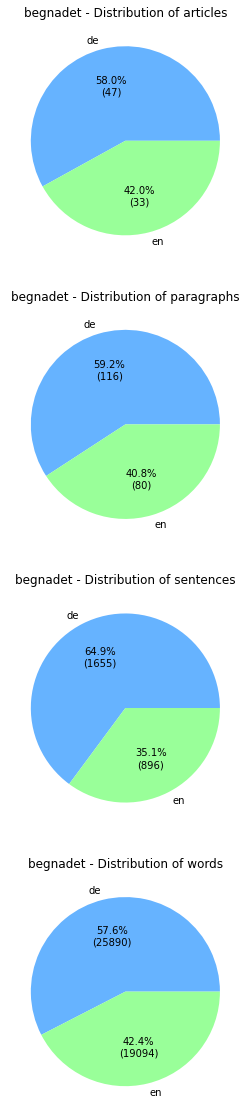
\includegraphics[width=.7\textwidth]{grafiken/Sprachverteilungen_begnadet_en_de.png}
        \caption{Sprachverteilungen Klasse „begnadet“}.
        \label{Sprachverteilungen_begnadet}
    \end{subfigure}%
    \begin{subfigure}[t]{.45\textwidth}
      \centering
        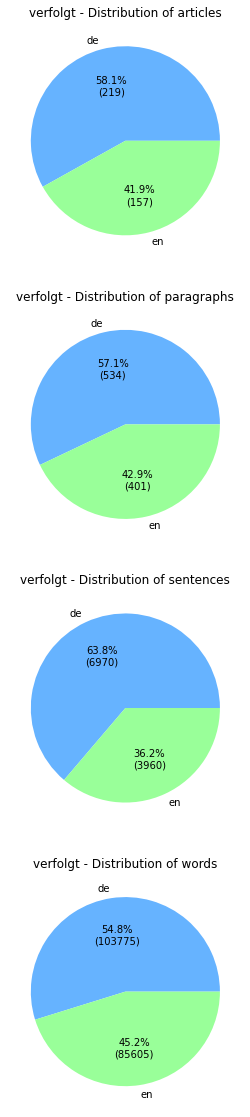
\includegraphics[width=.7\textwidth]{grafiken/Sprachverteilungen_verfolgt_en_de.png}
        \caption{Sprachverteilungen Klasse „verfolgt“}.
        \label{Sprachverteilungen_verfolgt}
    \end{subfigure}
\end{figure}

\chapter{Teilmenge der von BERTopic generierten Topic-Cluster}
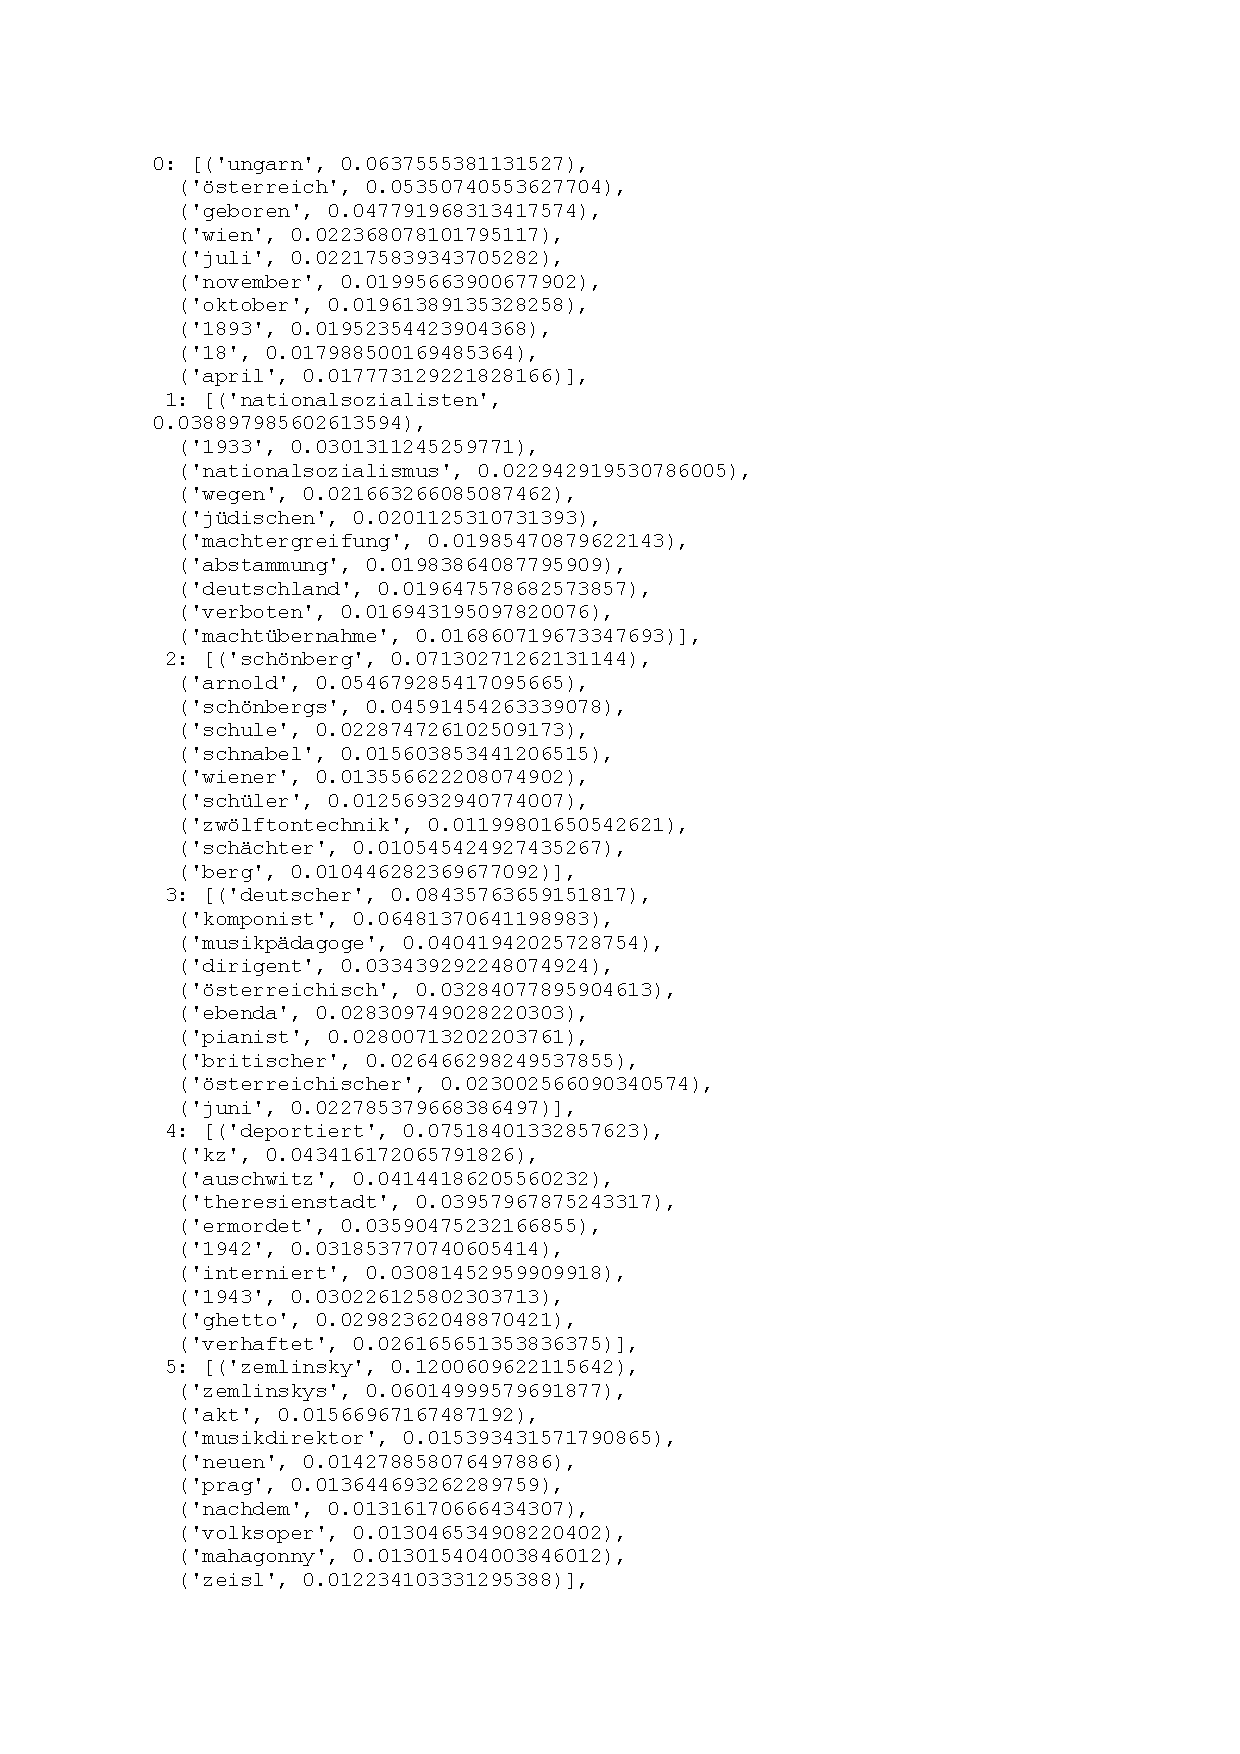
\includepdf[pages=-,pagecommand={},width=18cm]{26_topics_de_en.pdf}
\chapter{Vollständige Auswertungen der Textklassifikation mit Support Vector Machine und Naïve Bayes}
\newpage
\begin{table}[!ht]
    \centering
    \caption{Performanz der Textklassifikation mit Support Vector Machine und Naïve Bayes auf dem deutschen Datensatz}
    \begin{tabular}{|l|l|l|l|l|l|l|l|l|l|l|}
    \hline
        \textbf{} & \textbf{} & \textbf{} & \textbf{NB} & \textbf{} & \textbf{} & \textbf{} & \textbf{SVM} & \textbf{} & \textbf{} & \textbf{} \\ \hline
        Embeddings & Features & Res. & P & R & F1 & ACC & P & R & F1 & ACC \\ \hline
        W2V  & text  &   - & 0.52 & 0.54 & 0.52 & 0.72 & 0.50 & 0.39 & 0.44 & 0.78 \\ \hline
        W2V  & text  & Overs. & 0.61 & 0.58 & 0.52 & 0.54 & 0.56 & 0.62 & 0.31 & 0.31 \\ \hline
        W2V  & text  & Unders. & 0.59 & 0.56 & 0.49 & 0.50 & 0.57 & 0.44 & 0.44 & 0.58 \\ \hline
        W2V  & text + topics &   - & 0.50 & 0.41 & 0.45 & 0.81 & 0.50 & 0.41 & 0.45 & 0.81 \\ \hline
        W2V  & text + topics & Overs. & 0.45 & 0.49 & 0.41 & 0.54 & 0.44 & 0.48 & 0.40 & 0.52 \\ \hline
        W2V   & text + topics & Unders. & 0.29 & 0.41 & 0.34 & 0.52 & 0.44 & 0.48 & 0.40 & 0.52 \\ \hline
        fT  & text  &   - & 0.63 & 0.58 & 0.58 & 0.69 & 0.50 & 0.42 & 0.45 & 0.83 \\ \hline
        fT  & text  & Overs. & 0.62 & 0.57 & 0.57 & 0.67 & 0.67 & 0.60 & 0.58 & 0.67 \\ \hline
        fT  & text  & Unders. & 0.67 & 0.60 & 0.58 & 0.67 & 0.70 & 0.61 & 0.54 & 0.57 \\ \hline
        fT (a) & text  &   - & 0.50 & 0.50 & 0.46 & 0.63 & 0.50 & 0.41 & 0.45 & 0.81 \\ \hline
        fT  (a) & text  & Overs. & 0.54 & 0.52 & 0.46 & 0.57 & 0.62 & 0.55 & 0.49 & 0.59 \\ \hline
        fT  (a) & text  & Unders. & 0.51 & 0.51 & 0.46 & 0.52 & 0.51 & 0.51 & 0.46 & 0.52 \\ \hline
        fT (p,a) & text  &   - & 0.50 & 0.42 & 0.45 & 0.83 & 0.50 & 0.42 & 0.45 & 0.83 \\ \hline
        fT (p,a) & text  & Overs. & 0.79 & 0.69 & 0.71 & 0.80 & 0.83 & 0.77 & 0.79 & 0.87 \\ \hline
        fT (p,a) & text  & Unders. & 0.82 & 0.70 & 0.71 & 0.78 & 0.71 & 0.62 & 0.55 & 0.56 \\ \hline
        fT (p, a) & text + topics &  - & 0.57 & 0.66 & 0.57 & 0.80 & 0.50 & 0.40 & 0.44 & 0.80 \\ \hline
        fT (p, a) & text + topics & Overs. & 0.63 & 0.60 & 0.60 & 0.69 & 0.74 & 0.67 & 0.68 & 0.74 \\ \hline
        fT (p, a) & text + topics & Unders. & 0.60 & 0.57 & 0.56 & 0.63 & 0.64 & 0.61 & 0.47 & 0.48 \\ \hline
    \end{tabular}
\end{table}
\newpage\begin{table}[!ht]
    \centering
    \caption{Performanz der Textklassifikation mit Support Vector Machine und Naïve Bayes auf dem deutschen Datensatz}
    \begin{tabular}{|l|l|l|l|l|l|l|l|l|l|l|}
    \hline
        \textbf{} & \textbf{} & \textbf{} & \textbf{NB} & \textbf{} & \textbf{} & \textbf{} & \textbf{SVM} & \textbf{} & \textbf{} & \textbf{} \\ \hline
        Embeddings & Features & Res. & P & R & F1 & ACC & P & R & F1 & ACC \\ \hline
        W2V  & text  &   - & 0.48 & 0.38 & 0.43 & 0.74 & 0.50 & 0.38 & 0.43 & 0.77 \\ \hline
        W2V  & text  & Overs. & 0.53 & 0.53 & 0.53 & 0.64 & 0.50 & 0.50 & 0.40 & 0.41 \\ \hline
        W2V  & text  & Unders. & 0.54 & 0.53 & 0.50 & 0.54 & 0.55 & 0.54 & 0.47 & 0.49 \\ \hline
        W2V  & text + topics &   - & 0.50 & 0.42 & 0.46 & 0.85 & 0.50 & 0.42 & 0.46 & 0.85 \\ \hline
        W2V  & text + topics & Overs. & 0.66 & 0.58 & 0.50 & 0.54 & 0.59 & 0.59 & 0.31 & 0.31 \\ \hline
        W2V   & text + topics & Unders. & 0.58 & 0.54 & 0.46 & 0.51 & 0.50 & 0.08 & 0.13 & 0.15 \\ \hline
        fT  & text  &   - & 0.50 & 0.38 & 0.43 & 0.77 & 0.50 & 0.38 & 0.43 & 0.77 \\ \hline
        fT  & text  & Overs. & 0.52 & 0.51 & 0.43 & 0.44 & 0.52 & 0.51 & 0.43 & 0.44 \\ \hline
        fT  & text  & Unders. & 0.53 & 0.52 & 0.48 & 0.51 & 0.52 & 0.51 & 0.43 & 0.44 \\ \hline
        fT (a) & text  &   - & 0.50 & 0.38 & 0.43 & 0.77 & 0.40 & 0.38 & 0.43 & 0.77 \\ \hline
        fT  (a) & text  & Overs. & 0.57 & 0.56 & 0.46 & 0.46 & 0.53 & 0.62 & 0.26 & 0.28 \\ \hline
        fT  (a) & text  & Unders. & 0.51 & 0.51 & 0.46 & 0.49 & 0.57 & 0.56 & 0.46 & 0.46 \\ \hline
        fT (p,a) & text  &   - & 0.50 & 0.41 & 0.45 & 0.82 & 0.50 & 0.41 & 0.45 & 0.81 \\ \hline
        fT (p,a) & text  & Overs. & 0.65 & 0.65 & 0.65 & 0.79 & 0.62 & 0.60 & 0.61 & 0.74 \\ \hline
        fT (p,a) & text  & Unders. & 0.62 & 0.60 & 0.61 & 0.74 & 0.46 & 0.48 & 0.41 & 0.49 \\ \hline
        fT (p, a) & text + topics &  - & 0.50 & 0.41 & 0.45 & 0.82 & 0.50 & 0.41 & 0.45 & 0.82 \\ \hline
        fT (p, a) & text + topics & Overs. & 0.59 & 0.56 & 0.57 & 0.69 & 0.75 & 0.67 & 0.69 & 0.77 \\ \hline
        fT (p, a) & text + topics & Unders. & 0.65 & 0.60 & 0.60 & 0.69 & 0.61 & 0.61 & 0.36 & 0.36 \\ \hline
    \end{tabular}
\end{table}
\newpage
\begin{table}[!ht]
    \centering
    \caption{Performanz der Textklassifikation mit Support Vector Machine und Naïve Bayes auf dem multilingualen Datensatz}
    \begin{tabular}{|l|l|l|l|l|l|l|l|l|l|l|}
    \hline
        \textbf{} & \textbf{} & \textbf{} & \textbf{NB} & \textbf{} & \textbf{} & \textbf{} & \textbf{SVM} & \textbf{} & \textbf{} & \textbf{} \\ \hline
        Embeddings & Features & Res. & P & R & F1 & ACC & P & R & F1 & ACC \\ \hline
        W2V  & text  &   - & 0.47 & 0.48 & 0.47 & 0.65 & 0.50 & 0.42 & 0.46 & 0.85 \\ \hline
        W2V  & text  & Overs. & 0.50 & 0.50 & 0.45 & 0.54 & 0.47 & 0.48 & 0.44 & 0.54 \\ \hline
        W2V  & text  & Unders. & 0.50 & 0.50 & 0.46 & 0.55 & 0.43 & 0.47 & 0.40 & 0.49 \\ \hline
        W2V  & text + topics &   - & 0.48 & 0.48 & 0.48 & 0.77 & 0.50 & 0.42 & 0.46 & 0.85 \\ \hline
        W2V  & text + topics & Overs. & 0.53 & 0.52 & 0.47 & 0.55 & 0.53 & 0.52 & 0.47 & 0.55 \\ \hline
        W2V   & text + topics & Unders. & 0.61 & 0.56 & 0.51 & 0.59 & 0.39 & 0.44 & 0.40 & 0.57 \\ \hline
        fT  & text  &   - & 0.55 & 0.53 & 0.51 & 0.64 & 0.50 & 0.42 & 0.46 & 0.85 \\ \hline
        fT  & text  & Overs. & 0.60 & 0.55 & 0.50 & 0.57 & 0.64 & 0.57 & 0.50 & 0.54 \\ \hline
        fT  & text  & Unders. & 0.61 & 0.56 & 0.51 & 0.59 & 0.64 & 0.57 & 0.50 & 0.54 \\ \hline
        fT (a) & text  &   - & 0.52 & 0.51 & 0.52 & 0.73 & 0.50 & 0.42 & 0.46 & 0.85 \\ \hline
        fT  (a) & text  & Overs. & 0.52 & 0.51 & 0.43 & 0.49 & 0.59 & 0.57 & 0.35 & 0.35 \\ \hline
        fT  (a) & text  & Unders. & 0.52 & 0.51 & 0.42 & 0.8 & 0.60 & 0.59 & 0.33 & 0.33 \\ \hline
        fT (p,a) & text  &   - & 0.50 & 0.43 & 0.46 & 0.86 & 0.50 & 0.43 & 0.46 & 0.86 \\ \hline
        fT (p,a) & text  & Overs. & 0.59 & 0.55 & 0.54 & 0.68 & 0.69 & 0.60 & 0.59 & 0.68 \\ \hline
        fT (p,a) & text  & Unders. & 0.45 & 0.48 & 0.41 & 0.50 & 0.57 & 0.53 & 0.46 & 0.53 \\ \hline
        fT (p, a) & text + topics &  - & 0.56 & 0.58 & 0.57 & 0.80 & 0.50 & 0.42 & 0.46 & 0.85 \\ \hline
        fT (p, a) & text + topics & Overs. & 0.46 & 0.48 & 0.41 & 0.48 & 0.62 & 0.59 & 0.59 & 0.75 \\ \hline
        fT (p, a) & text + topics & Unders. & 0.42 & 0.46 & 0.36 & 0.41 & 0.48 & 0.49 & 0.44 & 0.52 \\ \hline
    \end{tabular}
\end{table}
\chapter{Vollständige Auswertungen der Textklassifikation mit BERT Modellen}
\newpage
\begin{table}[!ht]
    \centering
    \caption{Konfiguration und Performanz von gBERT auf dem deutschen Datensatz}
    \begin{tabular}{|l|l|l|l|l|l|l|l|}
    \hline
        \textbf{Epochen} & \textbf{Batchgröße} & \textbf{Lernrate} & \textbf{Loss} & \textbf{P} & \textbf{R} & \textbf{F1} & \textbf{Acc} \\ \hline
        1 & 8 & 3,00E-05 & 0.51 & 0.34 & 0.50 & 0.44 & 0.78 \\ \hline
        3 & 8 & 3,00E-05 & 0.40 & 0.85 & 0.94 & 0.87 & 0.90 \\ \hline
        5 & 8 & 3,00E-05 & 0.23 & 0.88 & 0.95 & 0.90 & 0.93 \\ \hline
        20 & 8 & 3,00E-05 & 0.07 & 0.91 & \textbf{0.97} & 0.93 & 0.95 \\ \hline
        1 & 16 & 3,00E-05 & 0.52 & 0.39 & 0.50 & 0.44 & 0.78 \\ \hline
        3 & 16 & 3,00E-05 & 0.50 & 0.39 & 0.50 & 0.44 & 0.78 \\ \hline
        5 & 16 & 3,00E-05 & 0.34 & 0.88 & 0.95 & 0.90 & 0.93 \\ \hline
        20 & 16 & 3,00E-05 & 0.10 & 0.91 & \textbf{0.97} & 0.93 & 0.95 \\ \hline
        5 & 8 & 5,00E-05 & 0.26 & 0.86 & 0.86 & 0.86 & 0.90 \\ \hline
        20 & 8 & 5,00E-05 & 0.07 & 0.88 & 0.95 & 0.90 & 0.93 \\ \hline
        1 & 16 & 5,00E-05 & 0.56 & 0.39 & 0.50 & 0.44 & 0.78 \\ \hline
        3 & 16 & 5,00E-05 & 0.48 & 0.39 & 0.50 & 0.44 & 0.78 \\ \hline
        5 & 16 & 5,00E-05 & 0.35 &\textbf{0.98} & 0.94 & \textbf{0.96} & \textbf{0.97} \\ \hline
        20 & 16 & 5,00E-05 & 0.09 & 0.82 & 0.92 & 0.85 & 0.88 \\ \hline
    \end{tabular}
\end{table}
\begin{table}[!ht]
    \centering
    \caption{Konfiguration und Performanz von mBERT auf dem deutschen Datensatz}
    \begin{tabular}{|l|l|l|l|l|l|l|l|}
    \hline
        \textbf{Epochen} & \textbf{Batchgröße} & \textbf{Lernrate} & \textbf{Loss} & \textbf{P} & \textbf{R} & \textbf{F1} & \textbf{Acc} \\ \hline
        1 & 8 & 3,00E-05 & 0.55 & 0.39 & 0.50 & 0.44 & 0.78 \\ \hline
        3 & 8 & 3,00E-05 & 0.50 & 0.39 & 0.50 & 0.44 & 0.78 \\ \hline
        5 & 8 & 3,00E-05 & 0.39 & 0.74 & 0.60 & 0.61 & 0.80 \\ \hline
        20 & 8 & 3,00E-05 & 0.44 & 0.39 & 0.50 & 0.44 & 0.78 \\ \hline
        1 & 16 & 3,00E-05 & 0.64 & 0.39 & 0.50 & 0.44 & 0.78 \\ \hline
        3 & 16 & 3,00E-05 & 0.57 & 0.39 & 0.50 & 0.44 & 0.78 \\ \hline
        5 & 16 & 3,00E-05 & 0.65 & 0.82 & 0.92 & 0.85 & 0.88 \\ \hline
        20 & 16 & 3,00E-05 & 0.13 & 0.56 & 0.52 & 0.51 & 0.75 \\ \hline
        5 & 8 & 5,00E-05 & 0.35 & 0.80 & 0.90 & 0.82 & 0.85 \\ \hline
        20 & 8 & 5,00E-05 & 0.10 & 0.83 & 0.80 & 0.81 & 0.88 \\ \hline
        1 & 16 & 5,00E-05 & 0.73 & 0.39 & 0.50 & 0.44 & 0.78 \\ \hline
        3 & 16 & 5,00E-05 & 0.43 & 0.39 & 0.50 & 0.44 & 0.78 \\ \hline
        5 & 16 & 5,00E-05 & 0.42 & 0.39 & 0.50 & 0.44 & 0.78 \\ \hline
        20 & 16 & 5,00E-05 & 0.13 & 0.85 & 0.90 & 0.87 & 0.90 \\ \hline
    \end{tabular}
\end{table}
\newpage
\begin{table}[!ht]
    \centering
    \caption{Konfiguration und Performanz von eBERT auf dem englischen Datensatz}
    \begin{tabular}{|l|l|l|l|l|l|l|l|}
    \hline
        \textbf{Epochen} & \textbf{Batchgröße} & \textbf{Lernrate} & \textbf{Loss} & \textbf{P} & \textbf{R} & \textbf{F1} & \textbf{Acc} \\ \hline
        1 & 8 & 3,00E-05 & 0.53 & 0.47 & 0.50 & 0.48 & 0.93 \\ \hline
        3 & 8 & 3,00E-05 & 0.58 & 0.47 & 0.50 & 0.48 & 0.93 \\ \hline
        5 & 8 & 3,00E-05 & 0.41 & 0.47 & 0.50 & 0.48 & 0.93 \\ \hline
        20 & 8 & 3,00E-05 & 0.11 & \textbf{0.75} &\textbf{0.96} &\textbf{0.81} &\textbf{0.93} \\ \hline
        1 & 16 & 3,00E-05 & 0.99 & 0.3 & 0.5 & 0.06 & 0.07 \\ \hline
        3 & 16 & 3,00E-05 & 0.66 & 0.47 & 0.50 & 0.48 & 0.93 \\ \hline
        5 & 16 & 3,00E-05 & 0.62 & 0.47 & 0.50 & 0.48 & 0.93 \\ \hline
        20 & 16 & 3,00E-05 & 0.19 & 0.73 & 0.73 & 0.73 & 0.93 \\ \hline
        5 & 8 & 5,00E-05 & 0.45 & 0.47 & 0.50 & 0.48 & 0.93 \\ \hline
        20 & 8 & 5,00E-05 & 0.13 & 0.65 & 0.71 & 0.67 & 0.90 \\ \hline
        1 & 16 & 5,00E-05 & 0.93 & 0.03 & 0.50 & 0.06 & 0.07 \\ \hline
        3 & 16 & 5,00E-05 & 0.65 & 0.47 & 0.50 & 0.48 & 0.93 \\ \hline
        5 & 16 & 5,00E-05 & 0.61 & 0.58 & 0.68 & 0.59 & 0.83 \\ \hline
        20 & 16 & 5,00E-05 & 0.17 & 0.73 & 0.73 & 0.73 & 0.93 \\ \hline
    \end{tabular}
\end{table}
\begin{table}[!ht]
    \centering
    \caption{Konfiguration und Performanz von mBERT auf dem englischen Datensatz}
    \begin{tabular}{|l|l|l|l|l|l|l|l|}
    \hline
        \textbf{Epochen} & \textbf{Batchgröße} & \textbf{Lernrate} & \textbf{Loss} & \textbf{P} & \textbf{R} & \textbf{F1} & \textbf{Acc} \\ \hline
        1 & 8 & 3,00E-05 & 0.58 & 0.47 & 0.50 & 0.48 & 0.93 \\ \hline
        3 & 8 & 3,00E-05 & 0.47 & 0.47 & 0.50 & 0.48 & 0.93 \\ \hline
        5 & 8 & 3,00E-05 & 0.46 & 0.73 & 0.73 & 0.73 & 0.93 \\ \hline
        20 & 8 & 3,00E-05 & 0.18 & 0.73 & 0.73 & 0.73 & 0.93 \\ \hline
        1 & 16 & 3,00E-05 & 0.70 & 0.47 & 0.50 & 0.48 & 0.93 \\ \hline
        3 & 16 & 3,00E-05 & 0.54 & 0.46 & 0.44 & 0.45 & 0.83 \\ \hline
        5 & 16 & 3,00E-05 & 0.57 & 0.47 & 0.50 & 0.48 & 0.93 \\ \hline
        20 & 16 & 3,00E-05 & 0.20 & 0.65 & 0.71 & 0.67 & 0.90 \\ \hline
        5 & 8 & 5,00E-05 & 0.44 & 0.46 & 0.44 & 0.45 & 0.83 \\ \hline
        20 & 8 & 5,00E-05 & 0.13 & 0.60 & 0.69 & 0.63 & 0.86 \\ \hline
        1 & 16 & 5,00E-05 & 0.68 & 0.46 & 0.46 & 0.46 & 0.86 \\ \hline
        3 & 16 & 5,00E-05 & 0.60 & 0.47 & 0.50 & 0.48 & 0.93 \\ \hline
        5 & 16 & 5,00E-05 & 0.55 & 0.47 & 0.50 & 0.48 & 0.93 \\ \hline
        20 & 16 & 5,00E-05 & 0.21 & 0.47 & 0.50 & 0.48 & 0.93 \\ \hline
    \end{tabular}
\end{table}
\newpage
\begin{table}[!ht]
    \centering
    \caption{Konfiguration und Performanz von mBERT auf dem multilingualen Datensatz}
    \begin{tabular}{|l|l|l|l|l|l|l|l|}
    \hline
        \textbf{Epochen} & \textbf{Batchgröße} & \textbf{Lernrate} & \textbf{Loss} & \textbf{P} & \textbf{R} & \textbf{F1} & \textbf{Acc} \\ \hline
        1 & 8 & 3,00E-05 & 0.51 & 0.41 & 0.50 & 0.45 & 0.81 \\ \hline
        3 & 8 & 3,00E-05 & 0.48 & 0.93 & 0.65 & 0.70 & 0.87 \\ \hline
        5 & 8 & 3,00E-05 & 0.38 & 0.85 & 0.89 & 0.89 & 0.91 \\ \hline
        15 & 8 & 3,00E-05 & 0.12 & 0.88 & 0.96 & 0.92 & 0.94 \\ \hline
        20 & 8 & 3,00E-05 & 0.38 & 0.88 & 0.96 & 0.92 & 0.94 \\ \hline
        1 & 16 & 3,00E-05 & 0.63 & 0.41 & 0.50 & 0.45 & 0.81 \\ \hline
        3 & 16 & 3,00E-05 & 0.44 & 0.83 & 0.94 & 0.86 & 0.90 \\ \hline
        5 & 16 & 3,00E-05 & 0.46 & 0.93 & \textbf{0.98} &\textbf{0.96} &\textbf{0.97} \\ \hline
        15 & 16 & 3,00E-05 & 0.14 & 0.89 & 0.88 & 0.88 & 0.93 \\ \hline
        20 & 16 & 3,00E-05 & 0.11 & 0.89 & 0.94 & 0.91 & 0.94 \\ \hline
        30 & 16 & 3,00E-05 & 0.08 & 0.86 & 0.86 & 0.86 & 0.91 \\ \hline
        5 & 8 & 5,00E-05 & 0.30 & 0.86 & 0.96 & 0.90 & 0.93 \\ \hline
        15 & 8 & 5,00E-05 & 0.15 & 0.85 & 0.89 & 0.87 & 0.91 \\ \hline
        20 & 8 & 5,00E-05 & 0.10 & 0.93 & \textbf{0.98} &\textbf{0.96} &\textbf{0.97} \\ \hline
        30 & 8 & 5,00E-05 & 0.14 & 0.91 & 0.94 & 0.91 & 0.94 \\ \hline
        1 & 16 & 5,00E-05 & 0.52 & 0.41 & 0.50 & 0.45 & 0.81 \\ \hline
        3 & 16 & 5,00E-05 & 0.44 & 0.83 & 0.94 & 0.86 & 0.90 \\ \hline
        5 & 16 & 5,00E-05 & 0.33 & 0.88 & 0.96 & 0.2 & 0.94 \\ \hline
        10 & 16 & 5,00E-05 & 0.20 & 0.93 & 0.88 & 0.90 & 0.94 \\ \hline
        15 & 16 & 5,00E-05 & 0.18 & 0.86 & 0.96 & 0.90 & 0.93 \\ \hline
        20 & 16 & 5,00E-05 & 0.16 & \textbf{0.98} & 0.89 & 0.92 & 0.96 \\ \hline
        30 & 16 & 5,00E-05 & 0.09 & 0.92 & 0.94 & 0.93 & 0.96 \\ \hline
    \end{tabular}
\end{table}
\listoffigures % Abbildungsverzeichnis
\listoftables % Tabellenverzeichnis
\renewcommand{\nomname}{Abkürzungsverzeichnis}
\printnomenclature % gebe Abkkürzungsverzeichnis aus
\printbibliography
\end{document}
